\documentclass[a4paper]{report}

\pagestyle{plain}
\usepackage{amssymb}
\usepackage{graphicx}
\usepackage{color}
\usepackage{amsfonts}
\usepackage{latexsym}
\usepackage{amsmath}
\usepackage[toc,page]{appendix}
\setcounter{tocdepth}{1}
\usepackage{pdfpages}
\usepackage{todonotes}
\usepackage{hyperref}
\hypersetup{
    colorlinks,
    citecolor=black,
    filecolor=black,
    linkcolor=black,
    urlcolor=black
}

\usepackage[authoryear]{natbib}
\usepackage{algorithm}
\usepackage{algpseudocode}

% \usepackage{caption}
\usepackage{subcaption}
\usepackage{float}
\usepackage{lipsum}
\usepackage[a4paper, margin = 3cm, bottom = 2.5cm]{geometry}


% ========================================
% Title Page
% ========================================
\title{{\vspace{-14em} 
\includegraphics[scale=0.4]{Logos/ucl_logo.png}}\\
{{\vspace{2em} \Huge Review of the Inverse $\mathcal{Z}$-Transform in the Pricing of Discrete Path-Dependent Options}}\\
{\large Final Year Project Report}\\
}
\date{Submission date: \today}
\author{Candidate Number: KCPD9\thanks{
{\bf Disclaimer:}
This report is submitted as part requirement for the MEng degree in Mathematical Computation at UCL. It is substantially the result of my own work except where explicitly indicated in the text. The report may be freely copied and distributed provided the source is explicitly acknowledged.}
\\ \\ Dr Carolyn Phelan
\\ \\ \\ \\ Department of Computer Science
\\ University College London
\\ \\
}



% ========================================
% Report
% ========================================
\begin{document}

\onehalfspacing
\maketitle

\renewcommand{\abstractname}{Acknowledgements}
\begin{abstract}
need to write something.
\end{abstract}

\renewcommand{\abstractname}{Abstract}
\begin{abstract}
\begin{itemize}
\item define notation for the entire project: $f(t) : \tilde{f}(z), f(t) : F(z), x(t) : X(z)$
\item Add more examples for completeness
\item follow Figure (XX) or (Figure XX)	
\item follow Section (XX) or (Section XX)
\item follow Eq. (XX) or (Equation XX)
\item follow Table (XX) or (Table XX)
\item follow Appendix (X) or (Appendix A)
\end{itemize}

\end{abstract}

% ========================================
% Contents
% ========================================
\tableofcontents
\setcounter{page}{1}

% ========================================
% Introduction
% ========================================
\chapter{Introduction}
\section{Motivation}
Standard (vanilla) options are the most basic and commonly traded type of options which give the holder the opportunity to buy or sell the asset at a later point in time. We attribute the first recorded option contract to that of the Greek philosopher Thales of Miletus \citep{thompson1994aristotle}. Believing that the olive harvest would be plentiful, Thales secured the right to use the olive presses at a low price. This agreement is considered a call option as it gives the holder the right, but not the obligation, to execute the contract at a predetermined price.

The formal study of pricing options began much later with \citet{bachelier1900theorie}'s work in modelling stock prices as a Brownian motion and his derivation of an option pricing formula. However, we deem the seminal work of \citet{black1973pricing} in laying out the foundation for modern option pricing theory. The introduction of the Black-Scholes model coincided with the establishment of the Chicago Board Options Exchange (CBOE) in 1973, which standardised option contracts and provided a platform for trading. The rapid growth (Fig \ref{fig:volume_of_options}) in the options market sparked a demand and increased interest in option pricing research.

\begin{figure}[h]
	\centering
	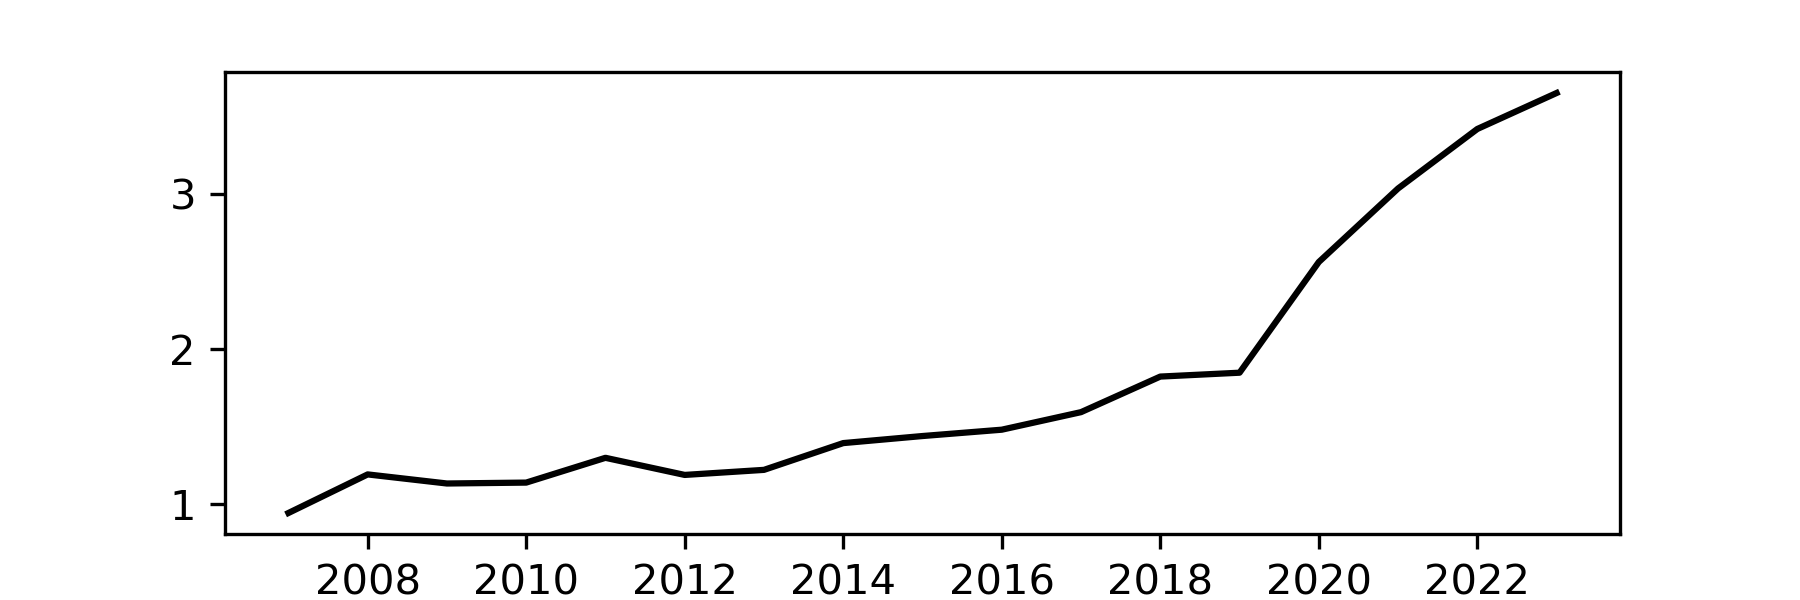
\includegraphics[width=0.7\linewidth]{images/options_volume.png}
	\captionsetup{justification=centering}
    \caption{Visualisation of the volume of options (in billions) traded over the past 17 years on exchanges CBOE, BATS, C2 and EDGX.}
    \label{fig:volume_of_options}
\end{figure}
However, the assumptions of the Black-Scholes model do not lend themselves to an accurate representation of real-world asset prices. Furthermore, exotic options differ in terms of their structure, payoff, and underlying asset to meet specific investor needs or market conditions. For instance, path-dependent options have payoffs determined by the path of the underlying asset price over the life of the option, rather than just the price at expiration. The price of the underlying asset is monitored at discrete points in time. One could say that in practice most, if not all, path-dependent options in markets are discrete path-dependent options \citep{kou2007discrete}.

The pricing of discrete path-dependent options has been a longstanding area of research in the financial mathematics literature. The importance and value of these options results in a vast array of research including that around the Black-Scholes model assumption \citep{lu2017improved, guardasoni2020mellin}, general L\'evy processes \citep{fang2009novel, fusai2016spitzer, phelan2018fourier, chen2021sinc, levendorskii2022sinh}, general Markov processes \citep{cui2021pricing, zhang2023general} and stochastic volatility \citep{soleymani2019pricing, kirkby2020efficient}.

A common problem faced by those in the literature is the linear dependency on the monitoring dates of the underlying asset price. \citet{fusai2016spitzer} demonstrated that the iteration on the monitoring dates can be avoided by working in the $z$-domain, extending on work by that of \citet{carr1999option}. Applying the \citet{spitzer1957wiener} identities and solving the resulting equations requires an inverse operation to obtain the option price. Reverting from the $z$-domain to the time domain requires a numerical approximation of the inverse $z$-transform. Despite its relation to the Fourier transform, the literature lacks in comparison; the performance of existing approximations, in terms of accuracy and efficiency, necessitates a specific setup and choice of parameters.

\section{Aims and Objectives}
Given the importance of the numerical inverse $z$-transform (NIZT), the focus of this project will be \textbf{(i)} studying the effect of the parameters on the varying methods, and \textbf{(ii)} testing on a group of well-defined transform pairs. Thus, our aim is to try and discover which methods provide the best fit in terms of efficiency and accuracy and what is the best setup to achieve this. The measurable objectives (O1-O5) associated with this aim are as follows:

\begin{itemize}
	\item (O1) Research into the pricing of options
	\item (O2) Research Boyarchenko and Levendorskii's new NIZT method (Sinh-Deformation)
	\item (O3) Analyse and implement the existing NIZT methods in literature
	\item (O4) Test the implementations against well-defined transform pairs
	\item (O5) Compute metrics on parameter setups for each method
\end{itemize}

\section{Overview}
The upcoming chapters of this report aims to provide a detailed description of the different stages taken through this project. In Chapter 2, we provide a self-contained technical background on the key concepts and methods used in this project. Given the breadth of the topic, references are included for those looking to delve deeper into the subject. In Chapter 3, we outline the experiments conducted in Chapter 4 to evaluate the performance of the numerical approximation methods. We detail the implementation of the methods and the experimental setup, including parameter selection and the benchmarking process. We then provide the results on a list of transform pairs and discuss the implications of the findings. Finally, Chapter 5 summarises the steps taken and the findings of this project with suggested work for further continuation. 

% ========================================
% Background
% ========================================
\chapter{Background}

In Chapter 2, we establish a foundational understanding of the topic in hand. This section is designed to be self-contained, providing essential background for all readers, while references are included for those seeking a deeper exploration.

We conduct an analysis into the mathematical concepts used in option pricing, with a focus on Fourier-based methods. While a large body of theoretical work exists in this area, the practical implementation of these methods is often computationally expensive, especially when evaluating high-dimensional integrals involved in the pricing formulas. We study literature on numerical approximation methods and the application in the pricing of exotic options, specifically lookback and barrier options. Subsequently, we explore the use-case of machine learning techniques to optimise parameters during our experimentation in Chapter 3.

% ========================================
% The Z-Transform
% ========================================
\section{The \texorpdfstring{$\mathcal{Z}$}{Lg}-Transform}\label{z_transform}

The $z$-transform is a transformation of a real or complex time function $x(n)$, often used for analysing discrete-time signals and systems. It is a generalisation of the discrete-time Fourier transform (DTFT) that extends the analysis to the complex plane. The bilateral Z-transform is formally defined as:

\begin{equation}\label{bilateral_z-transform}
X(z) = \mathcal{Z}_{n \rightarrow z}[x(n)] = \sum^{\infty}_{n = -\infty} x(n)z^{-n}
\end{equation}
``By definition, a complex number $z$ is an ordered pair $(x, y)$ of real numbers $x$ and $y$, written $z = (x, y)$'' \citep{kreyszig2010advanced}. In practice, complex numbers are written in the form $z = x + iy$, where $x$ and $y$ are real numbers and $i$ is the imaginary unit. We may find it easier to represent complex numbers in their polar form, $z = re^{i\theta}$, where $r$ represents the magnitude of $z$ and $\theta$ represents the angle of $z$ with respect to the positive real axis.

In the analysis of causal systems - systems for which a time origin is defined and is illogical to consider signal values for negative time - the unilateral $z$-transform is used. Unlike the bilateral $z$-transform in Eq. (\ref{bilateral_z-transform}), we sum from zero to positive infinity yielding

\begin{equation}\label{unilateral_z-transform}
X(z) = \mathcal{Z}_{n \rightarrow z}[x(n)] = \sum^{\infty}_{n = 0} x(n)z^{-n}
\end{equation}

The region within the complex $z$-plane where the $z$-transform converges is known as the Region of Convergence (ROC). The ROC is defined for the set of values of $z$ for which the $z$-transform is absolutely summable

\begin{equation}\label{roc}
\textbf{ROC} = \Biggl\{ z : \sum^{\infty}_{n = 0} |x(n)z^{-n}| < \infty \Biggr\}
\end{equation}

For causal sequences, the ROC is typically the exterior of the outermost pole in the $Z$-plane, denoted as $|z| > a$. If we say that $z_1$ converges, then $z_1$ exists within the ROC. Thus, all $z$ such that $|z| \geq |z_1|$ also converge. This region excludes the poles themselves, as the transform does not converge at those points. For the system to be $stable$, the ROC must include the unit circle, $|z| = 1$, implying that all poles must lie within the unit circle \citep{loveless2021guido}.

\begin{example}\label{example:roc_poles}
    Consider the function given by
    
    \begin{equation}
        H(z) = \frac{(z - i)(z + i)}{\left(z - \left(-\frac{1}{4} - \frac{1}{2}i\right)\right)\left(z - \left(\frac{1}{2} + \frac{1}{2}i\right)\right)}
    \end{equation}
    
    The ROC of $H(z)$ must exclude the poles at $z = -\frac{1}{4} - \frac{1}{2}i$ and $z = \frac{1}{2} + \frac{1}{2}i$, thus the ROC is $|z| > \frac{1}{2}$. The system is stable as the ROC includes the unit circle.

\end{example}

% ========================================
% Relation to Fourier Transform
% ========================================
\subsection{Relation to the Fourier Transform}\label{rs_fourier_transform}
It is useful to note the relationship between the $z$-transform and the Fourier transform. Taking the Fourier transform of a sampled function $x(t)$ results in:

\begin{flalign}
&& \mathcal{F}\bigg[x(t) \sum^{\infty}_{n = -\infty} \delta(t - n \Delta t)\bigg] &= \int^{\infty}_{-\infty} x(t) \sum_{n = - \infty}^{\infty} \delta (t - n\Delta t)e^{-i \omega t} dt && \\
&& &= \sum_{n = - \infty}^{\infty} \int^{\infty}_{-\infty} x(t) \delta (t - n\Delta t)e^{-i \omega t} dt && \\
&& &= \sum^{\infty}_{n=-\infty} x(n \Delta t)e^{-i \omega nt} &&
\end{flalign}

where we make use of the sifting property of the delta function. If we normalise the sampling interval to 1, we get

\begin{equation}\label{dtft}
\sum^{\infty}_{n = - \infty} x(n)e^{-i n \omega}
\end{equation}

This is the discrete-time Fourier transform (DTFT) of the sequence $x(n)$. The sequence $x(n)$ is sampled at discrete-time intervals $t_n = n \triangle t$, where the sampling interval $\triangle t$ is the time between consecutive samples and the time index $n$ numbers the samples. The DTFT is a periodic function of $\omega$ with period $2\pi$, and its existence relies on the absolute summability of the sequence $x(n)$:

\begin{equation}
\sum^{\infty}_{n = -\infty} |x(n)| < \infty
\end{equation}

The Z-transform generalises Eq. (\ref{dtft}) to the complex plane, not just the unit circle where $r = 1$ \citep{Oppenheim1989DTSP}.

% ========================================
% Relation to PDFs
% ========================================
\subsection{Relation to Probability Distribution Functions}\label{pdfs}
Random events and signals refer to situations where the outcome is not deterministic, but can be described by probability. Understanding these concepts involves using Probability Distribution Functions; the Probability Mass Function (PMF) for discrete random variables and the Probability Density Function (PDF) for continuous random variables. Given the nature of this project, we'll be focusing our attention on the PMF.

The PMF is defined for a discrete random variable $X$ taking on values $x_i$ with probabilities $p_i$, as $P(X=x_i) = p_i$. The PMF satisfies the following properties:

\begin{equation}
    \sum_{i=0}^n p_i = 1 \hspace{2em}\text{and}\hspace{2em} 0 \leq p_i \leq 1 \hspace{0.5em}\forall i
\end{equation}

We may find it useful to provide a concise representation of the entire distribution such that we expand upon the PMF, $p(x)$, to obtain the Probability Generating Function (PGF), $G_X(q)$, defined as

\begin{equation}
	G_X(q) = E[q^X] = \sum^{\infty}_{x = 0} p(x)q^x,
\end{equation}
where $E[\cdot]$ denotes the expectation operator, and $q$ is a complex number. We deliberately use $q$ to distinguish the PGF from the $z$-transform (Eqn. \ref{z_transform}).

% Example using a fair dice
\begin{example}
    Consider a fair six-sided dice. The PMF for the dice roll is given by
    
    \begin{equation}
        p(x) = \begin{cases}
            \frac{1}{6} & \text{if } x = 1, 2, 3, 4, 5, 6 \\
            0 & \text{otherwise}
        \end{cases}
    \end{equation}

    where $p(x)$ is the probability of rolling a number $x$. The PGF for the dice roll is then

    \begin{equation}
        G_X(q) = \sum^{\infty}_{x = 0} p(x)q^x = \frac{1}{6} \sum^6_{x = 1} q^x = \frac{q}{6}\cdot \frac{1-q^6}{1-q},
    \end{equation}

    where we use the formula for the sum of a geometric series. The PGF encapsulates the entire distribution of the dice roll into a single function.
\end{example}

The concept of summarising information is not unique to probability theory. In the analysis of signals, we aim to encapsulate the behaviour of a sequence into a single function. This is akin to the PGF, where the $z$-transform is used to analyse discrete-time signals and systems. Drawing on the principles outlined by \citet{ross2014introduction}, we can bridge the gap between probability theory and signal processing, leveraging the $z$-transform to analyse the behaviour of signals in the complex plane.

% ========================================
% The Inverse Z-Transform
% ========================================
\section{The Inverse \texorpdfstring{$\mathcal{Z}$}{Lg}-Transform}\label{section:inverse_z}
The inverse $Z$-transform aims to retrieve the sequence $x(n)$ from its $Z$-transform $X(z)$. While this transform is typically defined for finding individual values of $n$, it can also be extended to calculate the entire sequence. This is commonly defined by the Cauchy integral around a contour $C$ in the complex plane. The chosen contour $C$ is a counter-clockwise closed path that encloses the region of convergence (ROC) of $X(z)$. Formally, the inverse $Z$-transform is given by

\begin{equation}\label{inverse_z-transform}
	x(n) = \mathcal{Z}^{-1}_{z \rightarrow n}[X(z)] = \frac{1}{2\pi i} \oint_C X(z)z^{n-1}dz
\end{equation}

The integral approach enables the extraction of the complete sequence $x(n)$ for all integer values $n$, provided the ROC and the properties of $X(z)$ allow. In practical settings, numerical approximations are often used due to the computational challenges of evaluating the Cauchy integral. Whilst there are many ways to go about this \citep{merrikh2014linearsys, rajkovic2004method, horvath2020numerical}, most methods are done on a circular contour. Aligning with the focus of our project, we shift our attention to contour integrals.

% MAYBE: include other methods if we have time

% ========================================
% Abate and Whitt 1992
% ========================================
\subsection{Abate and Whitt 1992}\label{section:abate_whitt}
The numerical approximation formula offered by \citet{AbateWhitt1992a, AbateWhitt1992b} is based on a Fourier series catering to the inversion of probability generating functions as elucidated in Section \ref{pdfs}. The format is conducive to queuing theory and other probabilistic models where the $Z$-transform is defined as $q = 1 / z$. The authors approximate the inversion using a trapezoidal rule for numerical integration over a complex contour given by

\begin{equation}\label{aw_inversion_original}
	x(n) \approx \frac{1}{2nr^n} \biggr( X(r) + 2\sum^{n-1}_{k = 1} (-1)^k \mathrm{Re}\bigg( X(re^{\frac{ik\pi}{n}})\bigg) + (-1)^nX(-r) \biggl)
\end{equation}

The parameter $r$ is used to control the error; setting $r = 10^{-\lambda / 2n}$ yields an accuracy bound of $10^{-\lambda}$. The authors leverage the inherent symmetry within the complex plane to enhance computational efficiency by exploiting the complex conjugate symmetry of $X(z)$; each term $X(re^{\frac{ik\pi}{n}})$ in the upper half has a mirror image in the lower half. The computational load is thus halved by \textit{folding} the problem in this manner.

Given the nature of this project, we may find it easier to use the following definition, where we set the input of $X(z)$ to that of $z = 1 / q$, to approximate Eq. (\ref{inverse_z-transform}).

\begin{equation}\label{eq:aw_inversion}
	x(n) \approx \frac{1}{2nr^n} \biggr( X(\frac{1}{r}) + 2\sum^{n-1}_{k = 1} (-1)^k \text{Re}\bigg( X\big(\frac{1}{re^{\frac{ik\pi}{n}}}\big)\bigg) + (-1)^nX(-\frac{1}{r}) \biggl)
\end{equation}

The Nyquist-Shannon sampling theorem states that a signal must be sampled at a rate of at least twice the highest frequency present in the signal to avoid aliasing \citep{shannon1949communication,nyquist1928certain}. The number of points, $n$, used in Eq. (\ref{eq:aw_inversion}) must be sufficient to capture the information properly. If $n$ is too small, the approximation may lead to inaccuracies - akin to aliasing in signal processing.

% ========================================
% Cavers 1978
% ========================================
\subsection{Cavers 1978}\label{section:cavers}
Building on our analysis in Section (\ref{rs_fourier_transform}), \citet{Cavers1978FFT} proposes sampling the $z$-transform of a function on a circular contour at equally spaced points and then applying the inverse fast Fourier transform (IFFT) to these sampled points to approximate the original time-domain signal. The DTFT suffers from a high computational cost with a time complexity of O(N$^2$) given the need to perform O(N) operations for each of the N different points. Thus, the author employ a more efficient algorithm by \citet{cooley1965algorithm} to what is known as the fast Fourier transform (FFT), with a time complexity of O(NlogN). We can formulate this as:

\begin{equation}\label{cavers}
	x(n) = r^n \text{IFFT}[X(re^{2\pi ik / N})],
\end{equation}
which can be rewritten into the following:
\begin{equation}
		x(n) = \frac{r^n}{N} \text{FFT}[X(re^{2\pi ik / N})],
\end{equation}

where $r$ denotes the radius of the contour, $n$ is the time index, and $N$ is the number of points within the integration grid. The factor $r^n$ scales the result appropriately based on the radius of the contour. Recent studies, such as those by \citet{loveless2021guido}, show that increasing \(N\) results in an error tolerance approaching E-16, \textit{i.e. machine zero}, with double precision; note that this requires some optimisation of the chosen parameters. 

\citet{loveless2023phelanguido} explores replacing the IFFT of Eq. (\ref{cavers}) with a numerical summation over the grind points on half of the unit circle, similar to that of \citet{AbateWhitt1992a, AbateWhitt1992b}'s implementation. This is given as

\begin{equation}\label{equation:cavers_sum}
	x(n) = r^n \sum^{N}_{k = 1} X(re^{-\pi ik/N})
\end{equation}

The authors conclude that both implementations achieve machine-level accuracy of E-16 with some slight deviations and requiring an optimal hyperparameter setup.

% ========================================
% Optimisation Techniques
% ========================================
\section{Optimisation Techniques}\label{section:optimisation_techniques}
In the context of computational mathematics, optimisations techniques are used to identify the optimal or a sufficiently effective solution to a problem within a given set of constraints. The goal is to minimise or maximise a specific objective function by systematically choosing the values of the variables. The objective function is often referred to as the \textit{cost function} or \textit{loss function} and the variables are referred to as \textit{parameters}. The optimisation problem can be formulated as

\begin{equation}\label{optimisation_problem}
	\text{minimise } f(x) \text{ subject to } x \in \Omega,
\end{equation}
where $f(x)$ is the objective function and $\Omega$ is the feasible region defined by the constraints of the problem.

Gradient descent is one of the most popular algorithms for parameter optimisation with success in Deep Learning and Neural Networks employing variants of the algorithm \citep{lu2017improved, zhang2019gradient, zeebaree2019trainable}. The adaptability to diverse problem domains \citep{YingjieYugiHaibin2023SGD} parallels our use case, where gradient descent is applied outside traditional deep learning to optimise parameters of a mathematical function \citep{GradientBasedOpt2022}.

% ========================================
% Gradient Descent
% ========================================
\subsection{Gradient Descent}
Gradient descent iteratively converges to a local minimum of a function by moving in the direction of the steepest descent, as defined by the negative gradient. This method is expressed mathematically as

\begin{equation}\label{GD}
    x_{k+1} = x_k - \alpha_k \nabla f(x_k),
\end{equation}
where $x_k$ is the parameter vector at iteration $k$, $\alpha_k$ is the learning rate, and $\nabla f(k)$ represents the gradient of the function at $x_k$. The selection of $\alpha_k$ determines the size of the step taken towards the minimum; too large can overshoot the minimum, too small can result in a long convergence time. The process repeats until a predetermined termination criterion is met, typically when the change in the value of $f(k)$ falls below a threshold. This iterative process is showcased in the pseudocode below:

\begin{algorithm}
\caption{Gradient Descent}
\label{algo:gradient_descent}
\begin{algorithmic}[1]
\State Initialise \( x_0 \), set \( k = 0 \)
\While{termination conditions not met}
    \State $g_k$ = \( \nabla f(x_k) \) \Comment Compute Gradient
    \State $\alpha_k \rightarrow \mathbb{R}^+$
    \State $x_{k+1} = x_k - \alpha_k g_k$
    \State \( k = k + 1 \)
\EndWhile
\end{algorithmic}
\end{algorithm}

% ========================================
% Stochastic Gradient Descent
% ========================================
\subsubsection{Stochastic Gradient Descent}
However, classic Gradient Descent faces limitations, including susceptibility to local minima. Stochastic Gradient Descent (SGD) addresses this by introducing variability in the optimisation process. It modifies Eq.~(\ref{GD}) to use a randomly selected subset of data to compute the gradient, leveraging noise to escape local minima. We define the update rule to 

\begin{equation}\label{SGD}
x_{k+1} = x_k - \alpha_k \nabla f_{i_k}(x_k)	
\end{equation}
where $\nabla f_{i_k}(x_k)$ is the gradient of the cost function with respect to a random subset $i_k$.

% ========================================
% Adam Optimizer
% ========================================
\subsubsection{ADAM Optimizer}\label{section:ADAM}
ADAM (Adaptive Moment Estimation) is a popular optimisation algorithm introduced by \citet{kingma2014adam} that combines the advantages of two extensions to the stochastic gradient descent method: AdaGrad \citep{duchi2011adaptive} and RMSProp \citep{tieleman2012rmsprop}. ADAM computes adaptive learning rates for each parameter by estimating the first and second moments of the gradients. This makes the method particularly well-suited for large-scale and complex optimisation problems, such as those countered in deep learning and computational optimisation. It's ability to adjust learning rates based on gradient information allows ADAM to efficiently navigate the parameter space and converge to extremely precise solutions \citep{reddi2019convergence}. The update rule is given by:

\begin{equation}
x_{k+1} = x_{k} - \alpha \frac{\hat{m}_{k}}{\sqrt{\hat{v}_{k}} + \epsilon},
\end{equation}
where first moment estimate $m_k$ and the second moment estimate $v_k$ are computed as exponential moving averages of the gradient and the squared gradient, respectively. The hyperparameters $\beta_1$ and $\beta_2$ control the decay rates of these moving averages. To correct for initialisation bias, the estimates of the first and second moments ($\hat{m}_k$and $\hat{v}_k$) are bias-corrected. The parameter update is performed using the adapted learning rate $\alpha$ and the bias-corrected estimates of the moments. We add $\epsilon$ to the denominator to prevent division be zero; typically set to $10^{-8}$. This process is shown in the pseudocode below:

\begin{algorithm}[H]
\caption{ADAM Optimizer}
\label{algo:ADAM}
\begin{algorithmic}[1]
\State Initialise \( x_0 \), \( m_0 = 0 \), \( v_0 = 0 \), set \( k = 0 \)
\State Hyperparameters: \( \alpha \), \( \beta_1 \), \( \beta_2 \), \( \epsilon \)
\While{termination conditions not met}
    \State \( k = k + 1 \)
    \State \( g_k = \nabla f(x_k) \) \Comment Compute Gradient
    \State \( m_k = \beta_1 m_{k-1} + (1 - \beta_1) g_k \)
    \State \( v_k = \beta_2 v_{k-1} + (1 - \beta_2) g_k^2 \)
    \State \( \hat{m}_k = \frac{m_k}{1 - \beta_1^k} \) \Comment Bias-Corrected First Moment
    \State  \( \hat{v}_k = \frac{v_k}{1 - \beta_2^k} \) \Comment Bias-Corrected Second Moment
    \State \( x_{k+1} = x_k - \alpha \frac{\hat{m}_k}{\sqrt{\hat{v}_k} + \epsilon} \)
\EndWhile
\end{algorithmic}
\end{algorithm}

% ========================================
% Option Pricing
% ========================================
\section{Option Pricing}\label{section:option_pricing}
The concept involves determining the value of options, which are financial contracts that give the holder the right, \textit{but not the obligation}, to buy or sell an asset at a set price, $K$ (strike price), within a specified time-frame, $T$ (expiration date). The value of an option, $V$, is derived from the underlying asset, denoted as $S$, which can be a stock, bond, or commodity. This relationship can be mathematically expressed as:
\begin{equation}
	V = f(S, K, T, \sigma, r),
\end{equation}
where $\sigma$ represents the volatility of the underlying asset\footnotemark[1] and $r$ is the risk-free interest rate\footnotemark[2].

\footnotetext[1]{A measure of how much the price of the asset is expected to fluctuate over a certain period of time.}
\footnotetext[2]{The interest rate at which an invest can lend money with virtually no risk of loss.}

A pivotal point in option pricing was the introduction of \citet{black1973pricing}'s model in estimating the price of European-style options, which can only be exercised at the expiration date. The Black-Scholes model is based on the assumption that the price of the underlying asset follows a geometric Brownian motion in idealistic conditions. However, many options traded in real markets are American-style, allowing the holder to exercise the option at any time before the expiration date. This complicates the pricing process as it involves solving an \textit{optimum stopping problem}. \citet{merton1973theory} extends the Black-Scholes model to American options by expressing the price as the solution to a free boundary problem. While Merton's work provided a theoretical foundation, solving the free boundary problem analytically is challenging. Instead, numerical methods such as binomial trees \citep{cox1979option} and simulation-based methods \citep{longstaff2001simulation} have been developed to price American options.

% ========================================
% Path-Dependent Options
% ========================================
\subsection{Path-Dependent Options}\label{section:discrete_monitoring}
We regard American and European options as standard (\textit{vanilla}) options. In contrast, exotic options offer more complex features and conditions that can be tailored to meet specific needs and/or requirements. Such differences are the reason as to why exotic options are traded over-the-counter (OTC)\footnotemark[3], whereas standard options are typically traded on organised exchanges\footnotemark[4]. 

\footnotetext[3]{Over-The-Counter refers to the process of trading of financial instruments directly between two parties without the oversight of a formal exchange.}
\footnotetext[4]{Organised exchanges refer to formal marketplaces that facilitate the buying and selling of financial instruments.}

In most cases, the payoff of an option depends on the price of the underlying asset at discrete points in time rather than continuously. This is known as \textbf{discrete monitoring.} Two widely traded types of discretely monitored options are lookback and barrier options \citep{dadachanji2015fx}. These options are classified as \textit{path-dependent options}, within the category of exotic options, where the payoff is based on the path of the underlying asset price rather than just the price at expiration.

\subsubsection{Lookback Options}\label{lookback}
\begin{figure}[H]
    \begin{subfigure}{.5\linewidth}
      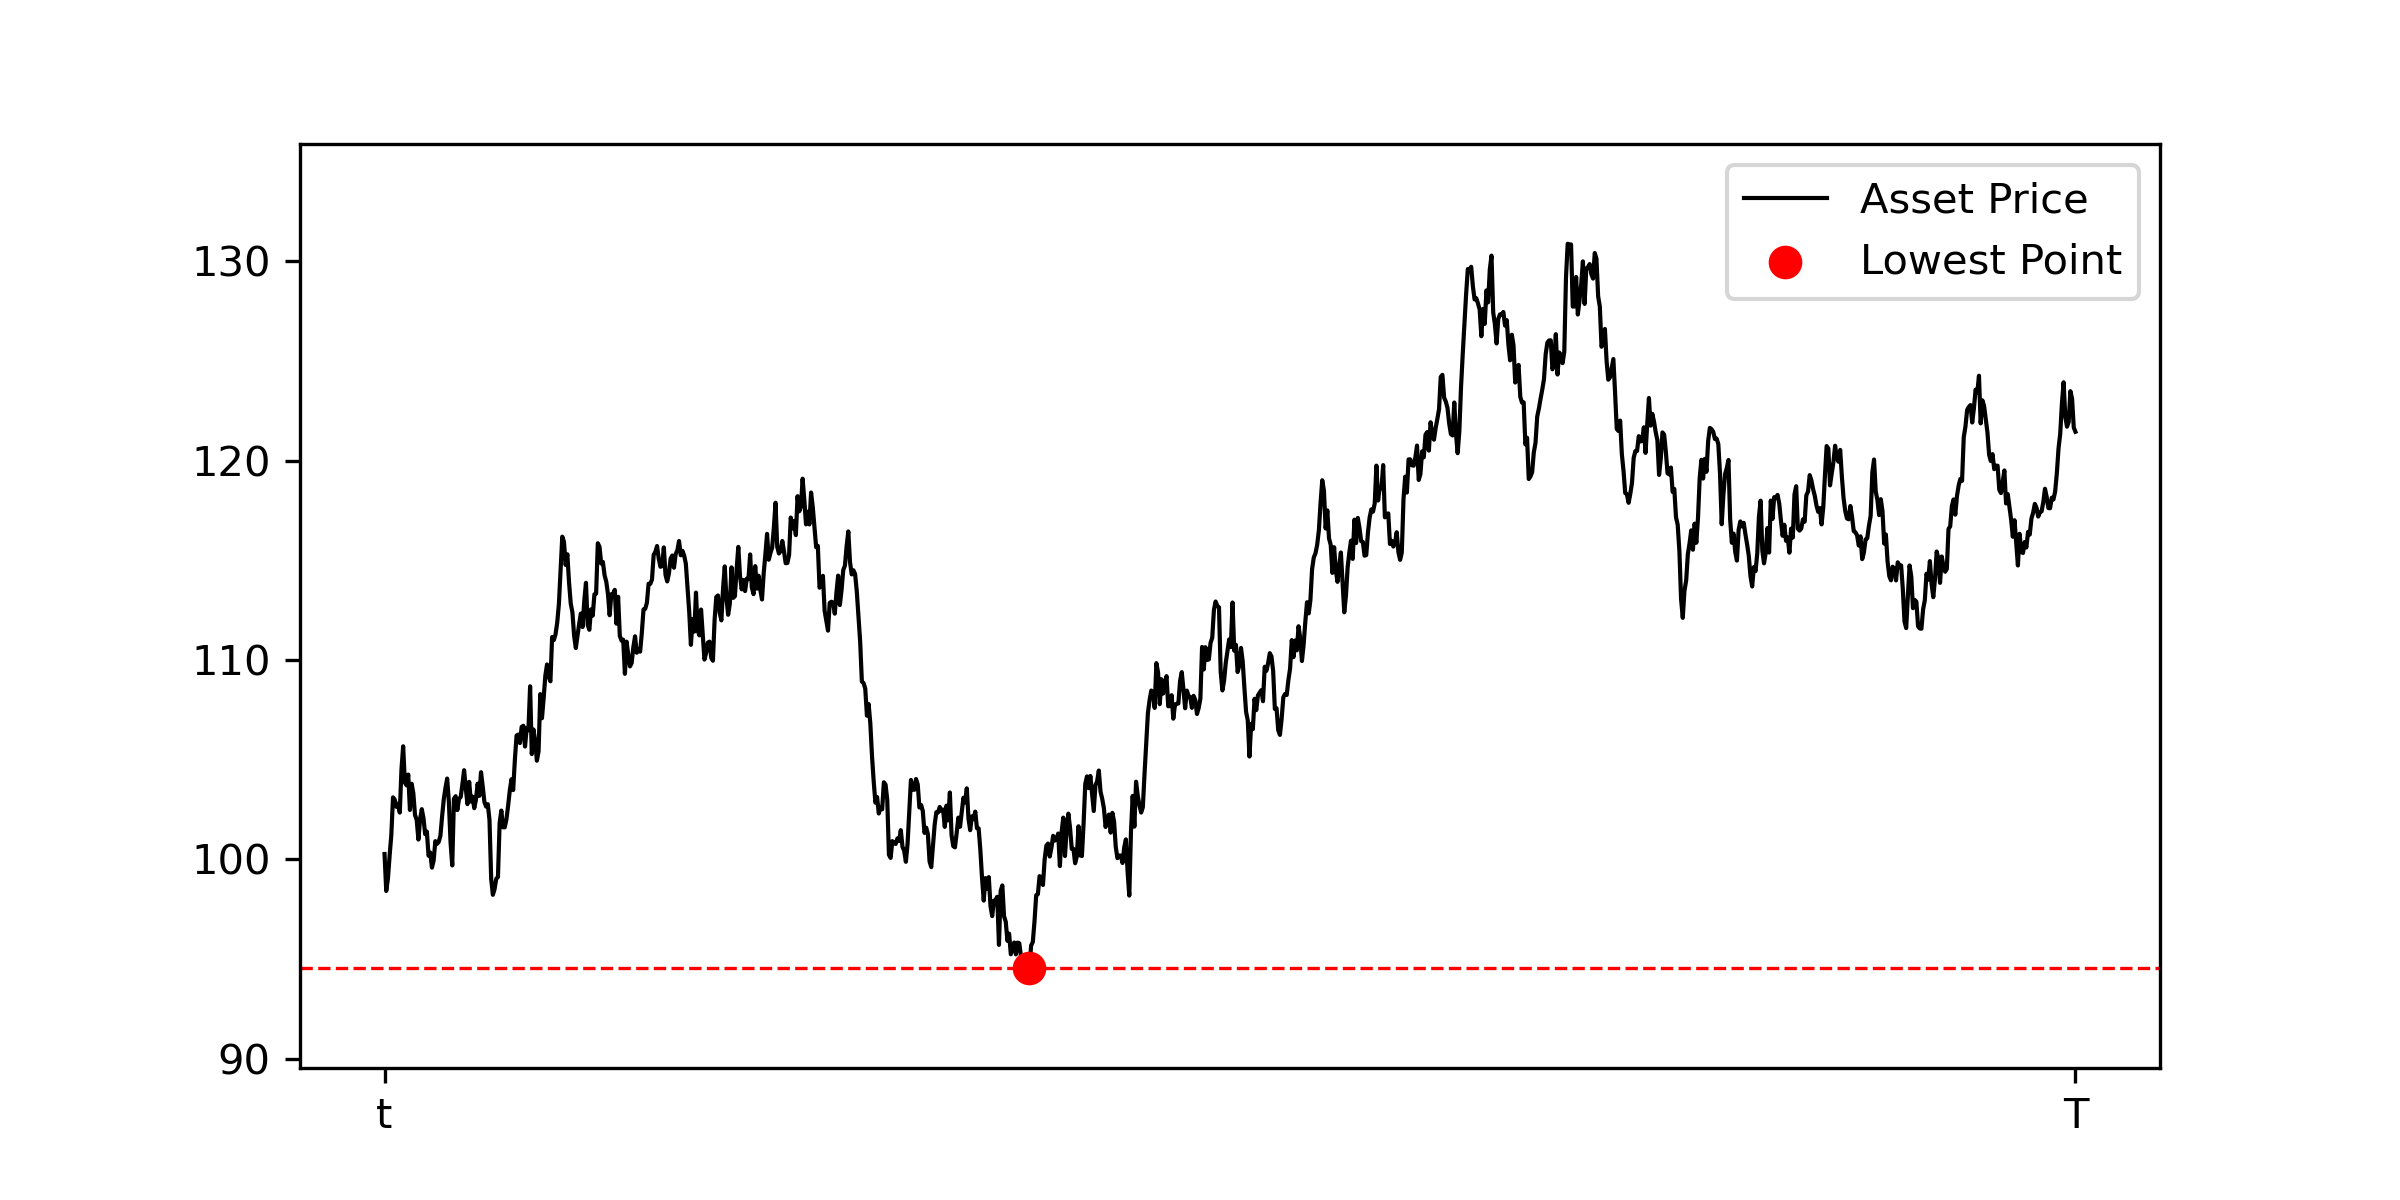
\includegraphics[width=\linewidth]{images/call_option.png}
      \caption{Lookback Call Option}
      \label{fig:call_option}
    \end{subfigure}\hfill
    \begin{subfigure}{.5\linewidth}
      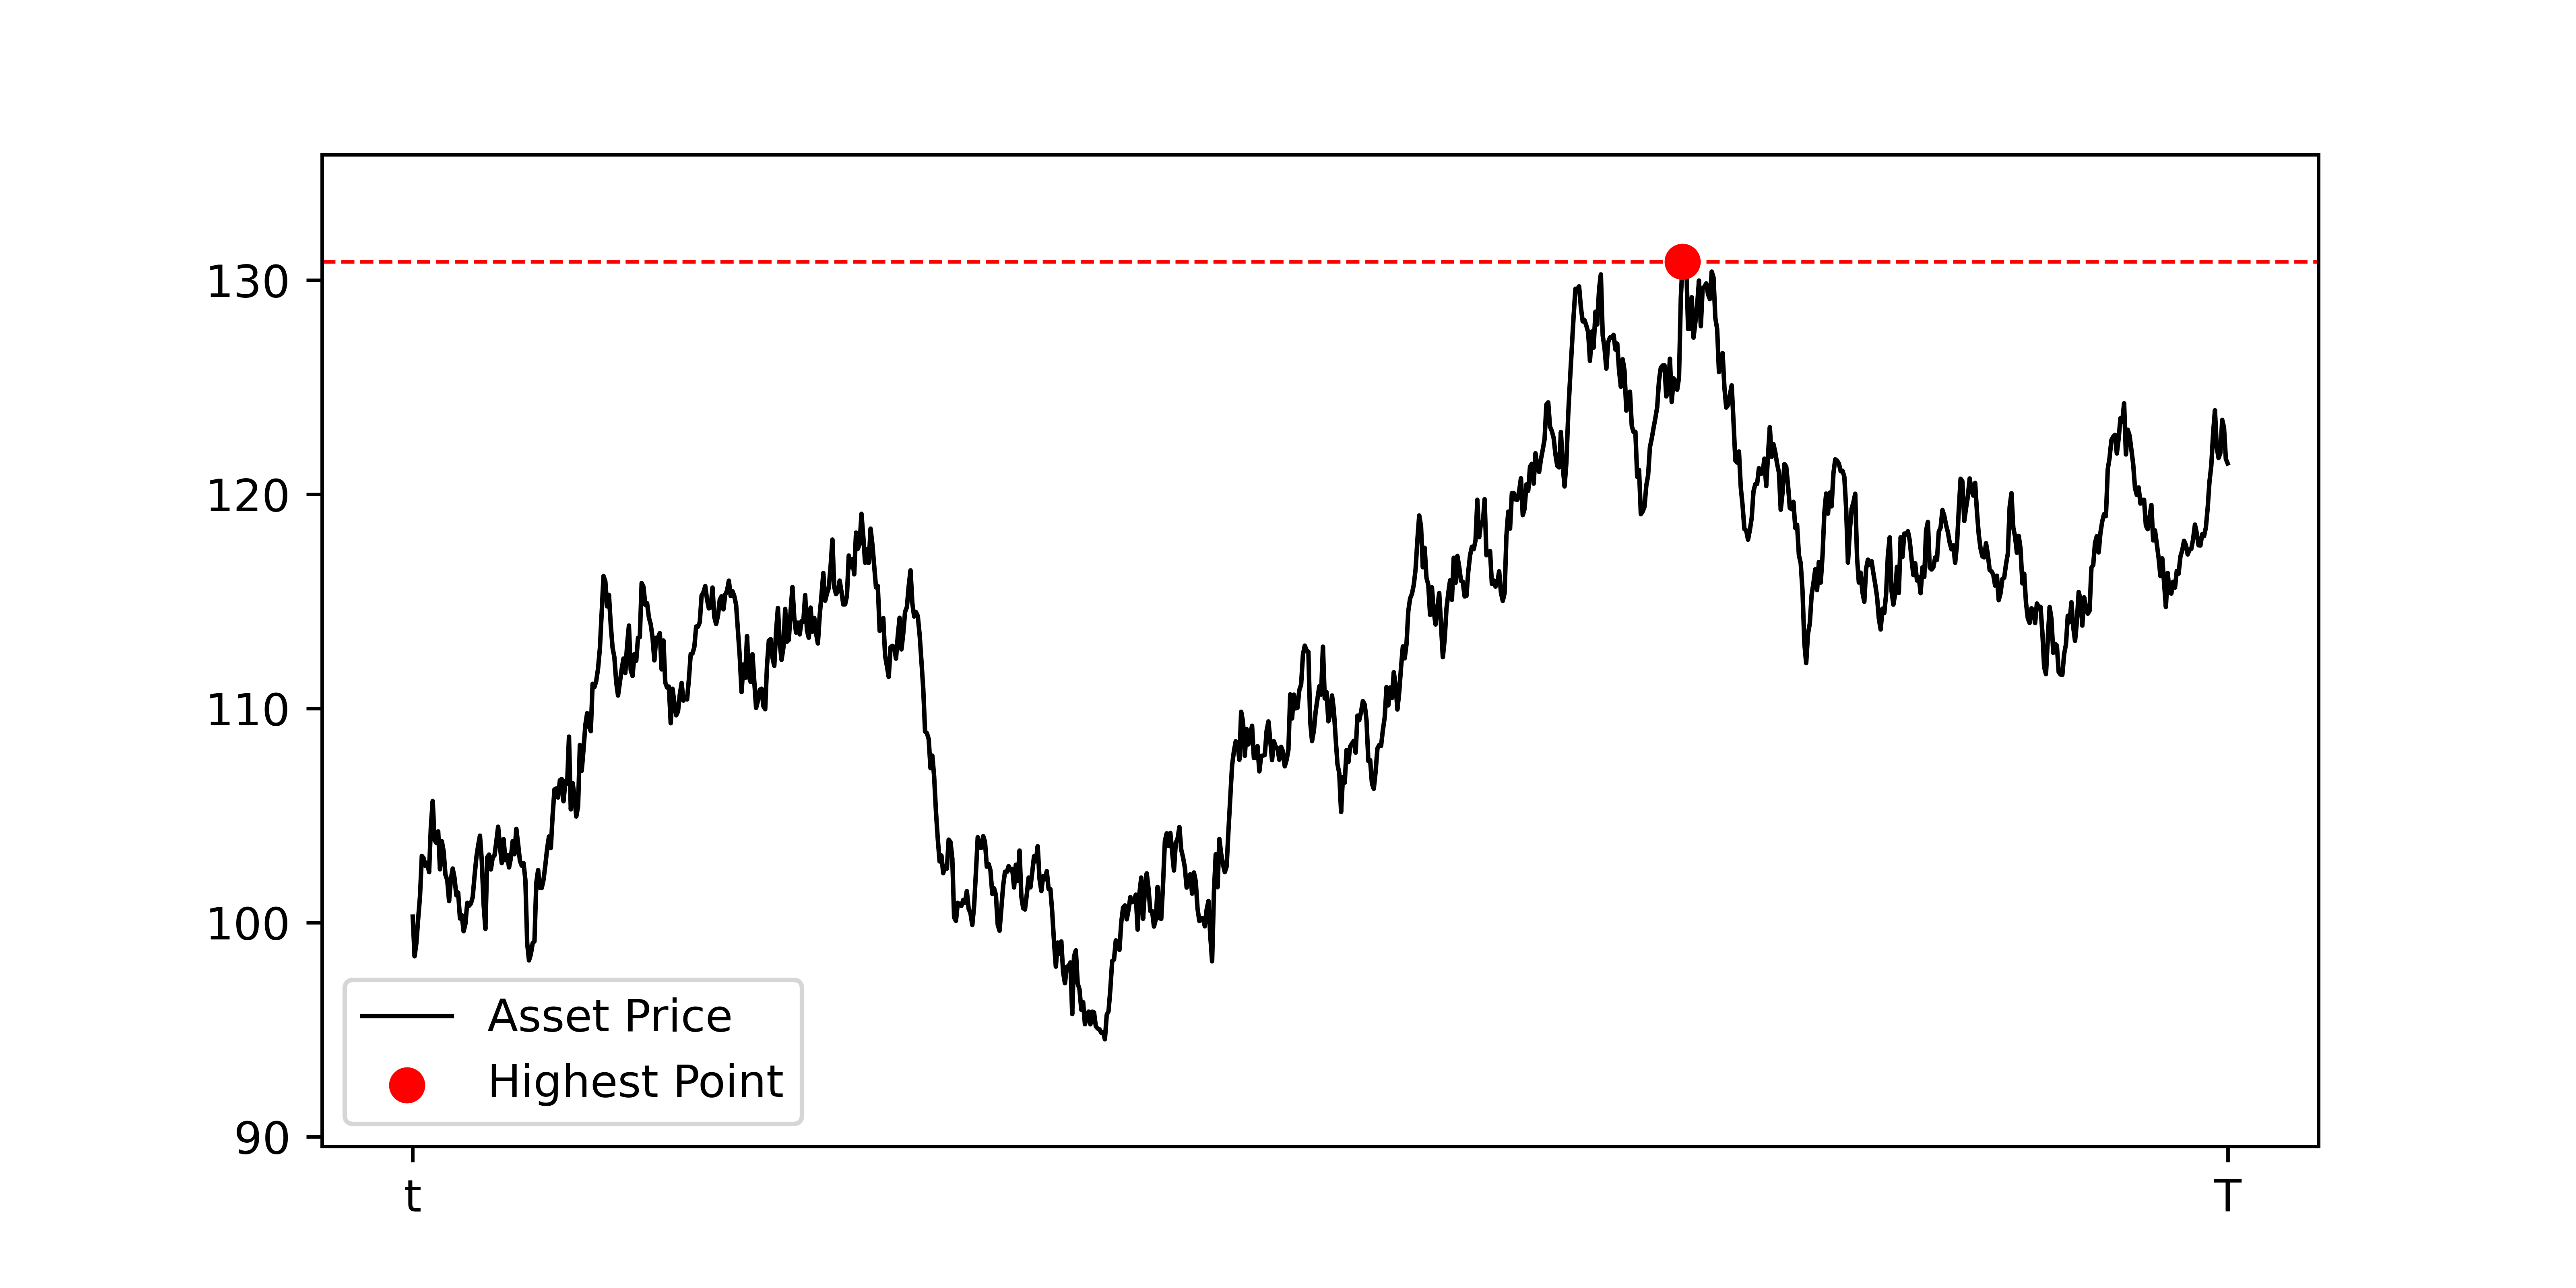
\includegraphics[width=\linewidth]{images/put_option.png}
      \caption{Lookback Put Option}
      \label{fig:put_option}
    \end{subfigure}
    \caption{Illustration of Lookback Options: Displaying the mechanics of (a) Call Option and (b) Put Option. The red line represents the barrier, while the red dot marks the strike price.}
\end{figure}

\noindent The payoff depends on the maximum and minimum asset price over the life of the option. A \textit{lookback call option} (\autoref{fig:call_option}) gives the holder the right to buy the asset at the lowest price during the option period, while a \textit{lookback put option} (\autoref{fig:put_option}) allows the holder to sell the asset at the highest price during the option period.

\subsubsection{Barrier Options}\label{barrier}
\begin{figure}[H]
    \begin{subfigure}{.5\linewidth}
      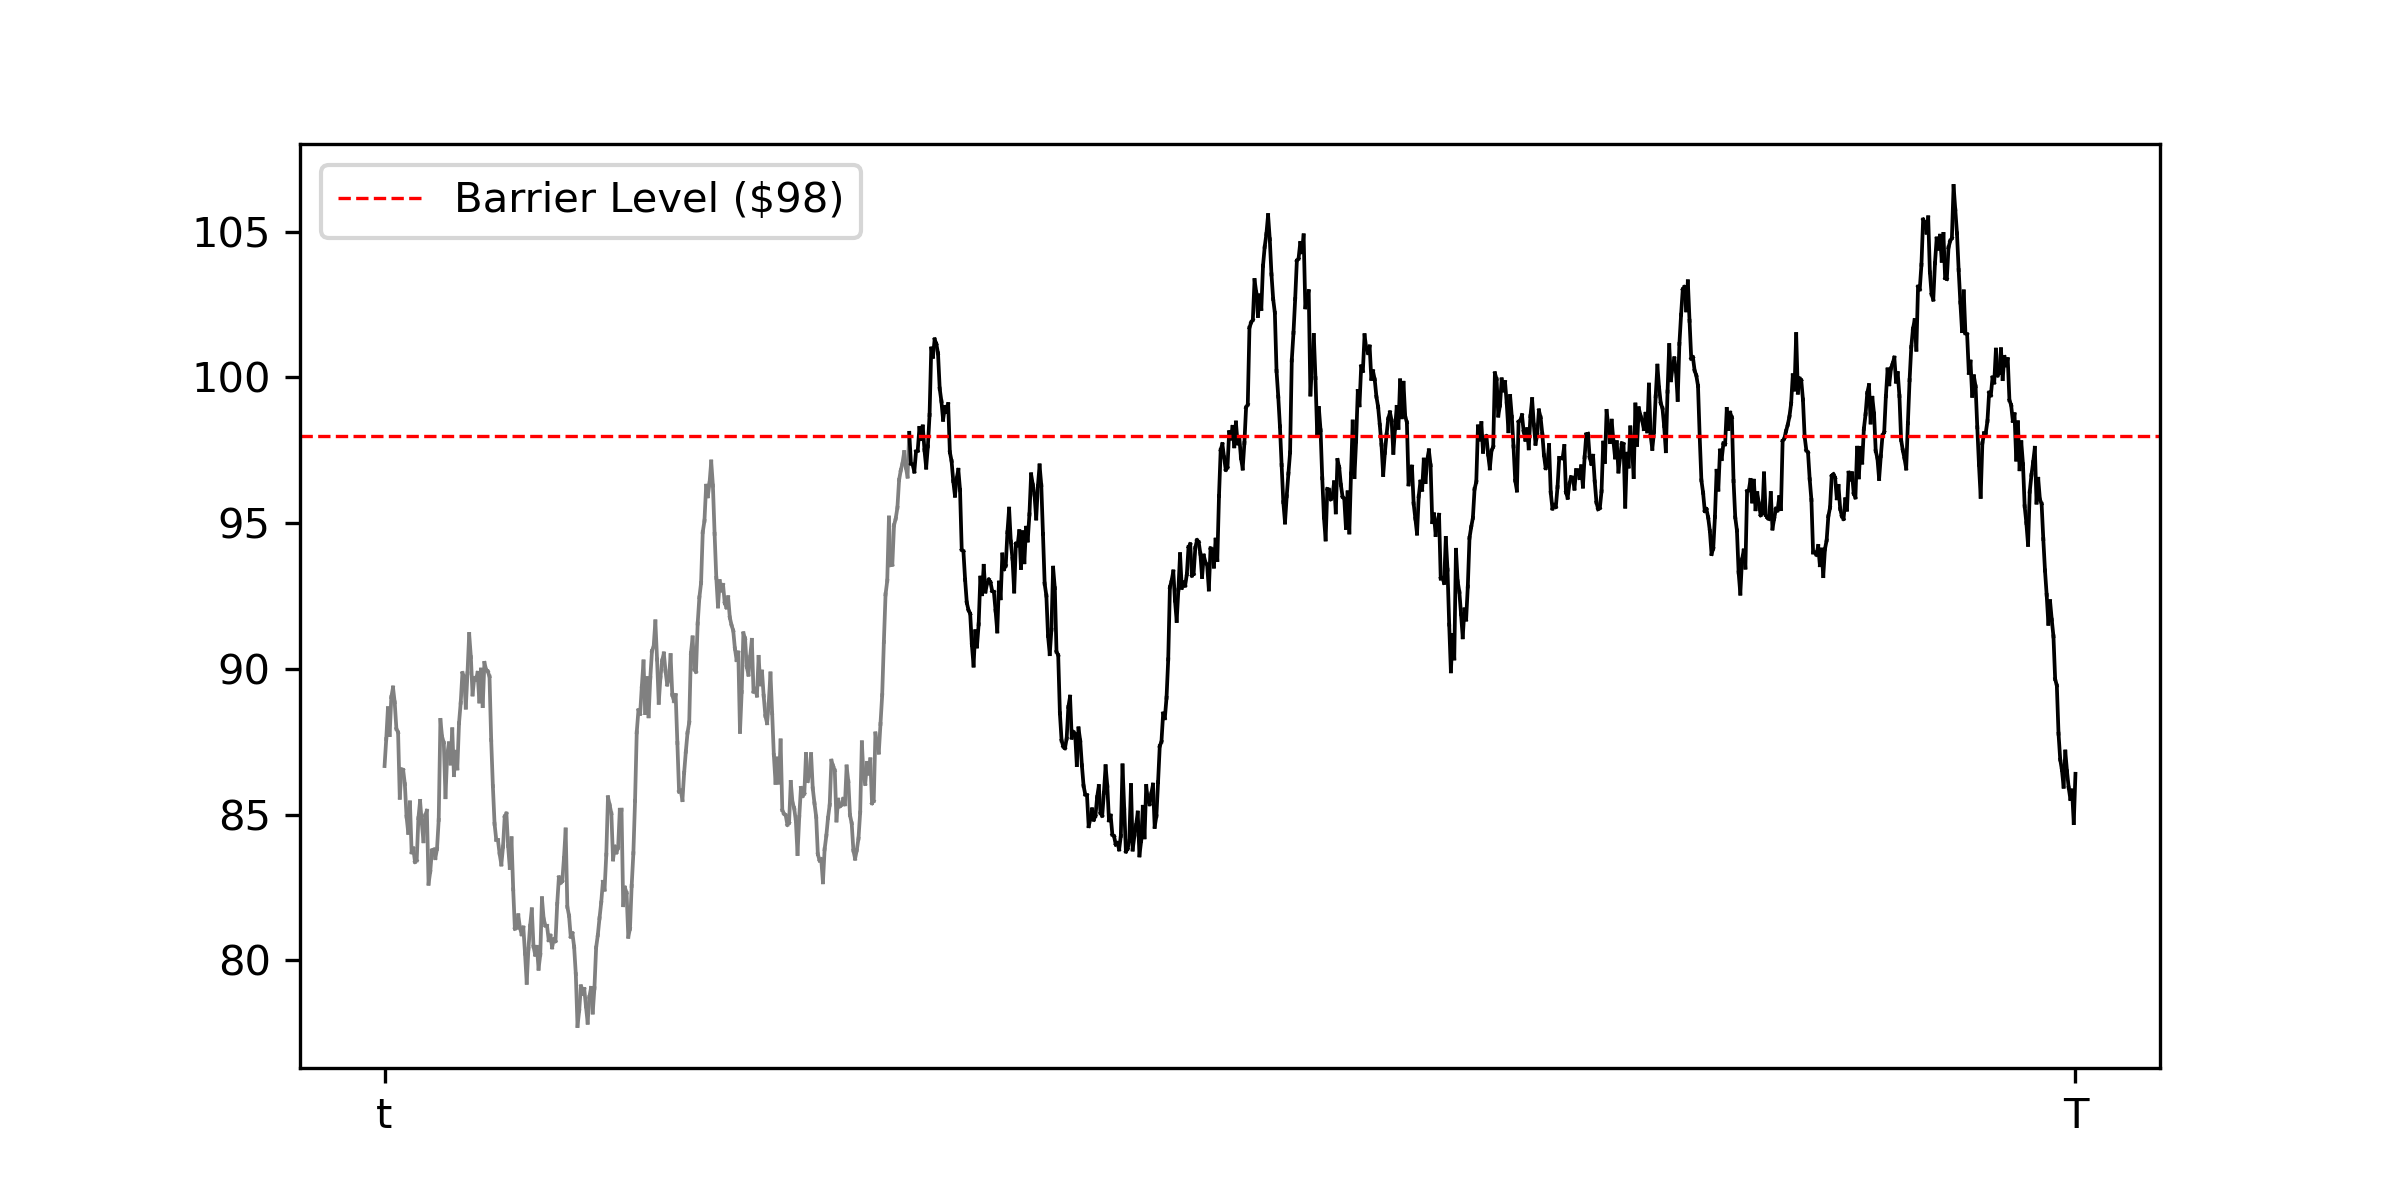
\includegraphics[width=\linewidth]{images/up_in_option.png}
      \caption{Up-and-In Barrier Option}
      \label{fig:up_in_option}
    \end{subfigure}\hfill
    \begin{subfigure}{.5\linewidth}
      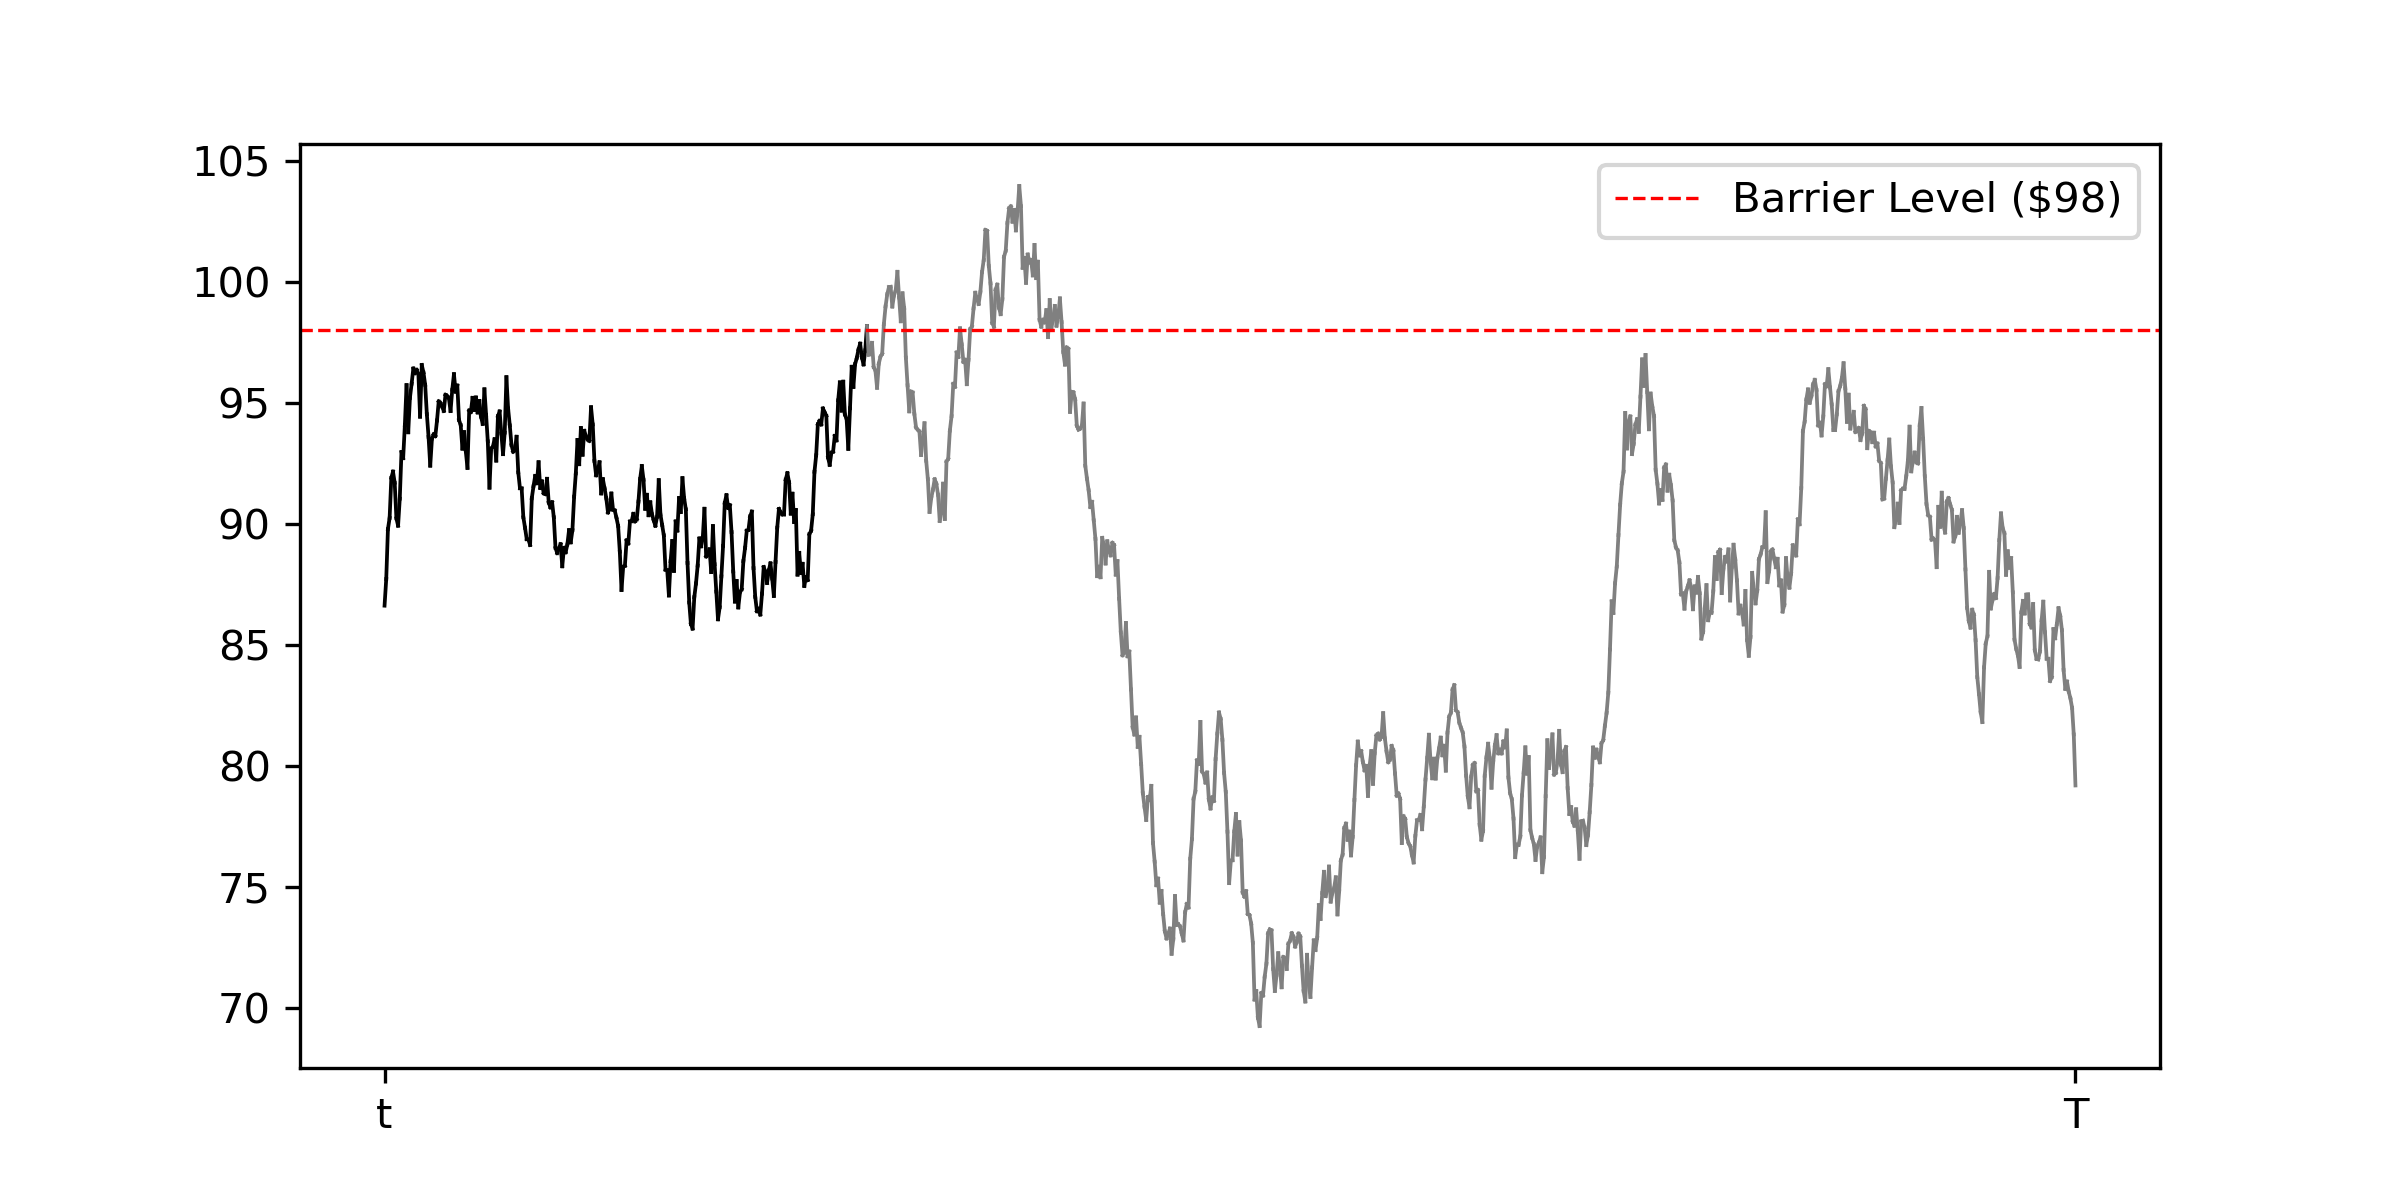
\includegraphics[width=\linewidth]{images/up_out_option.png}
      \caption{Up-and-Out Barrier Option}
      \label{fig:up_out_option}
    \end{subfigure}
    
    \medskip
    \begin{subfigure}{.5\linewidth}
      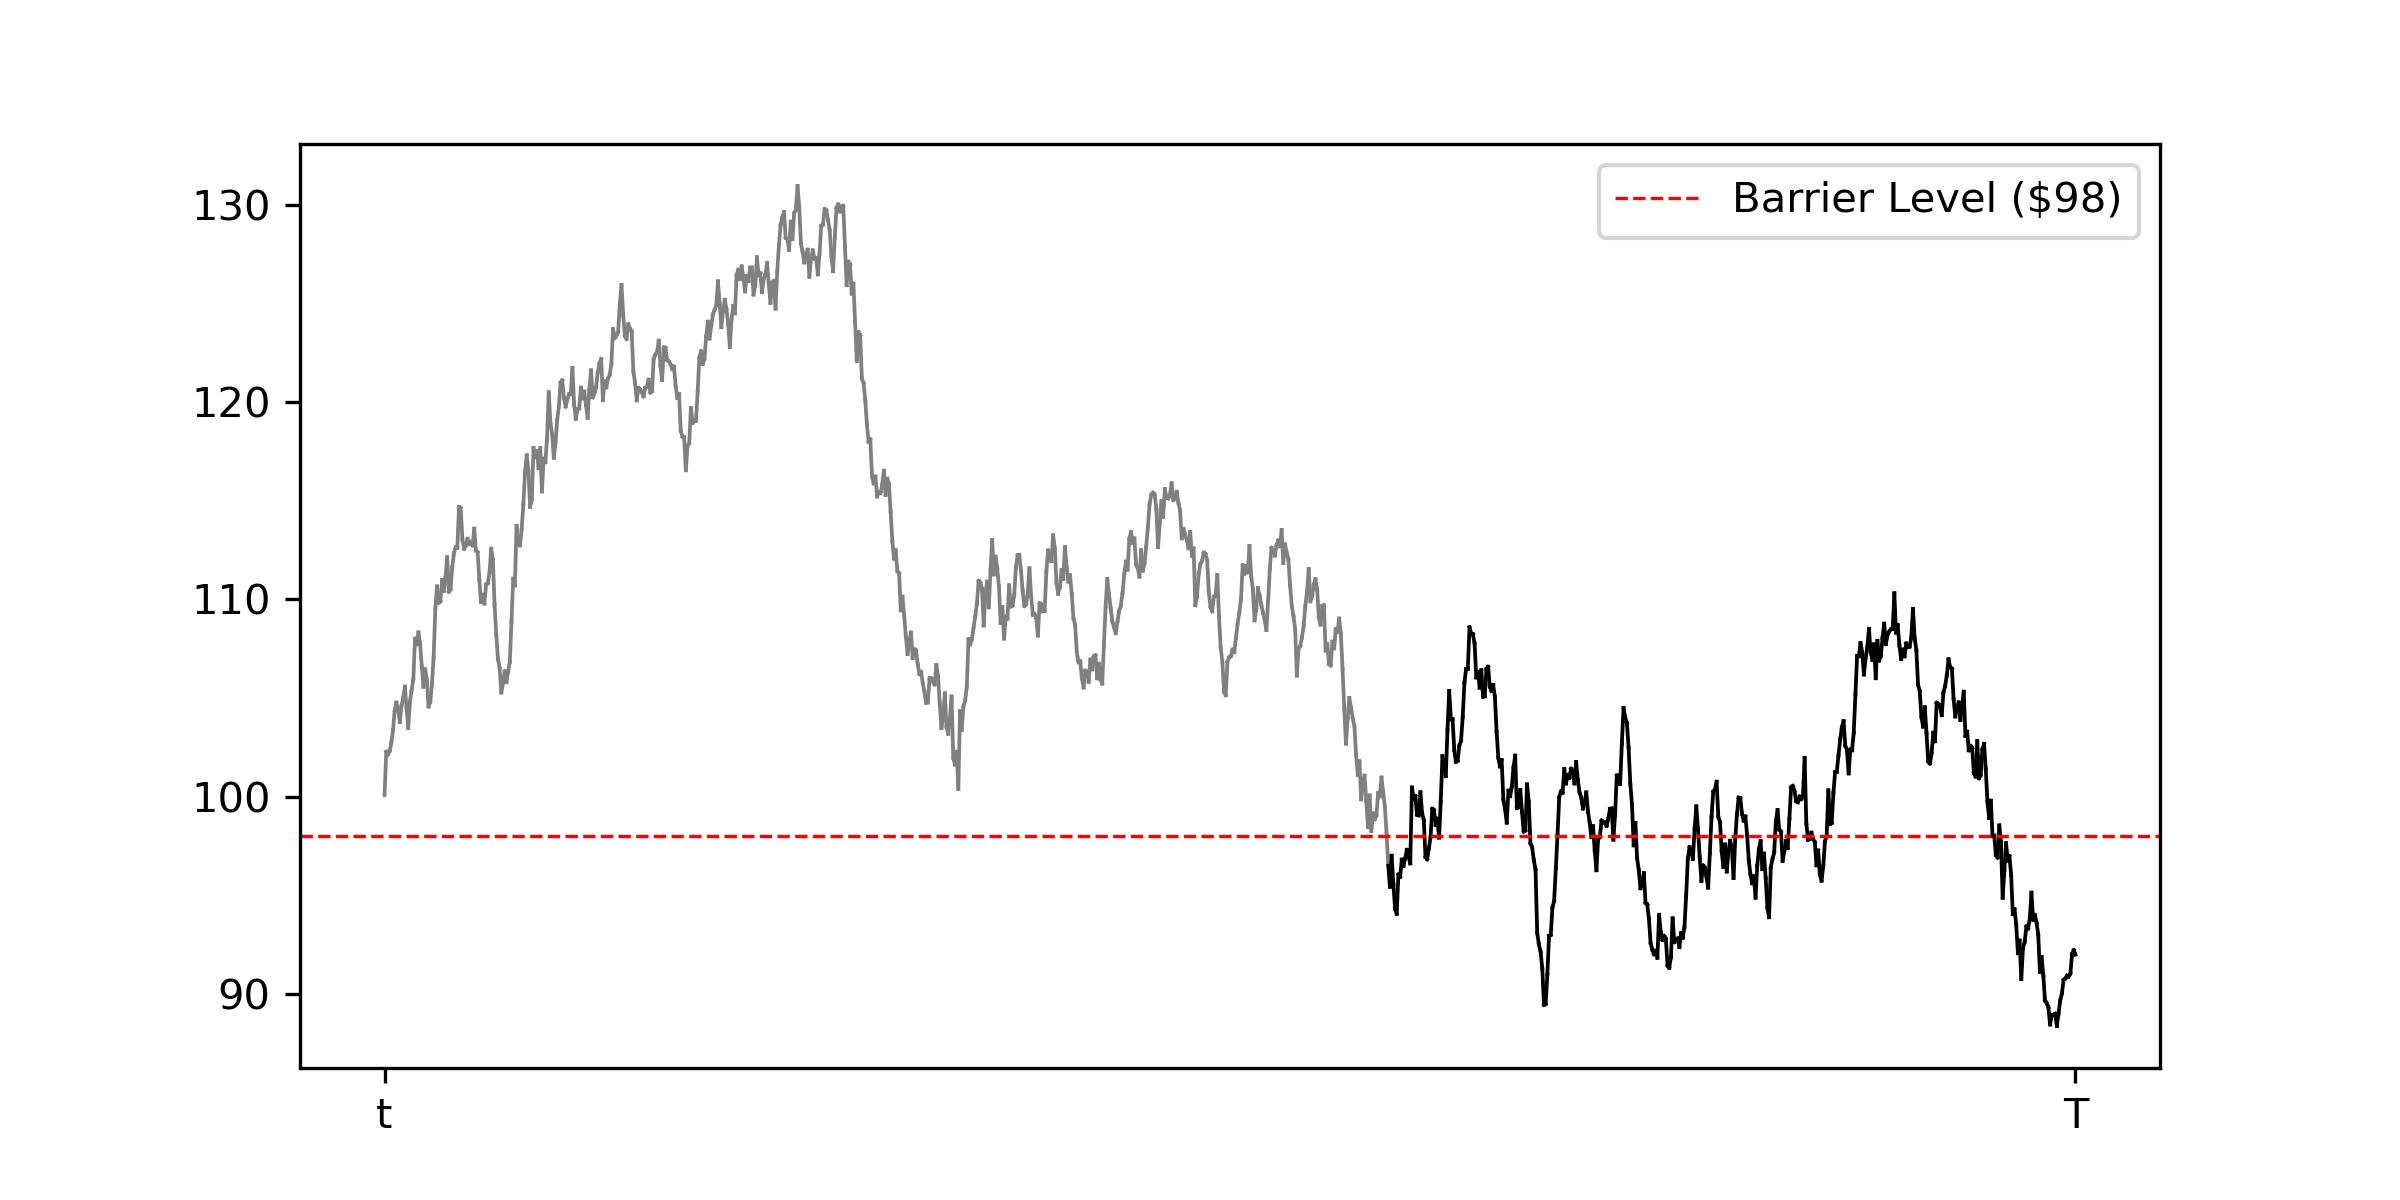
\includegraphics[width=\linewidth]{images/down_in_option.png}
      \caption{Down-and-In Barrier Option}
      \label{fig:down_in_option}
    \end{subfigure}\hfill
    \begin{subfigure}{.5\linewidth}
      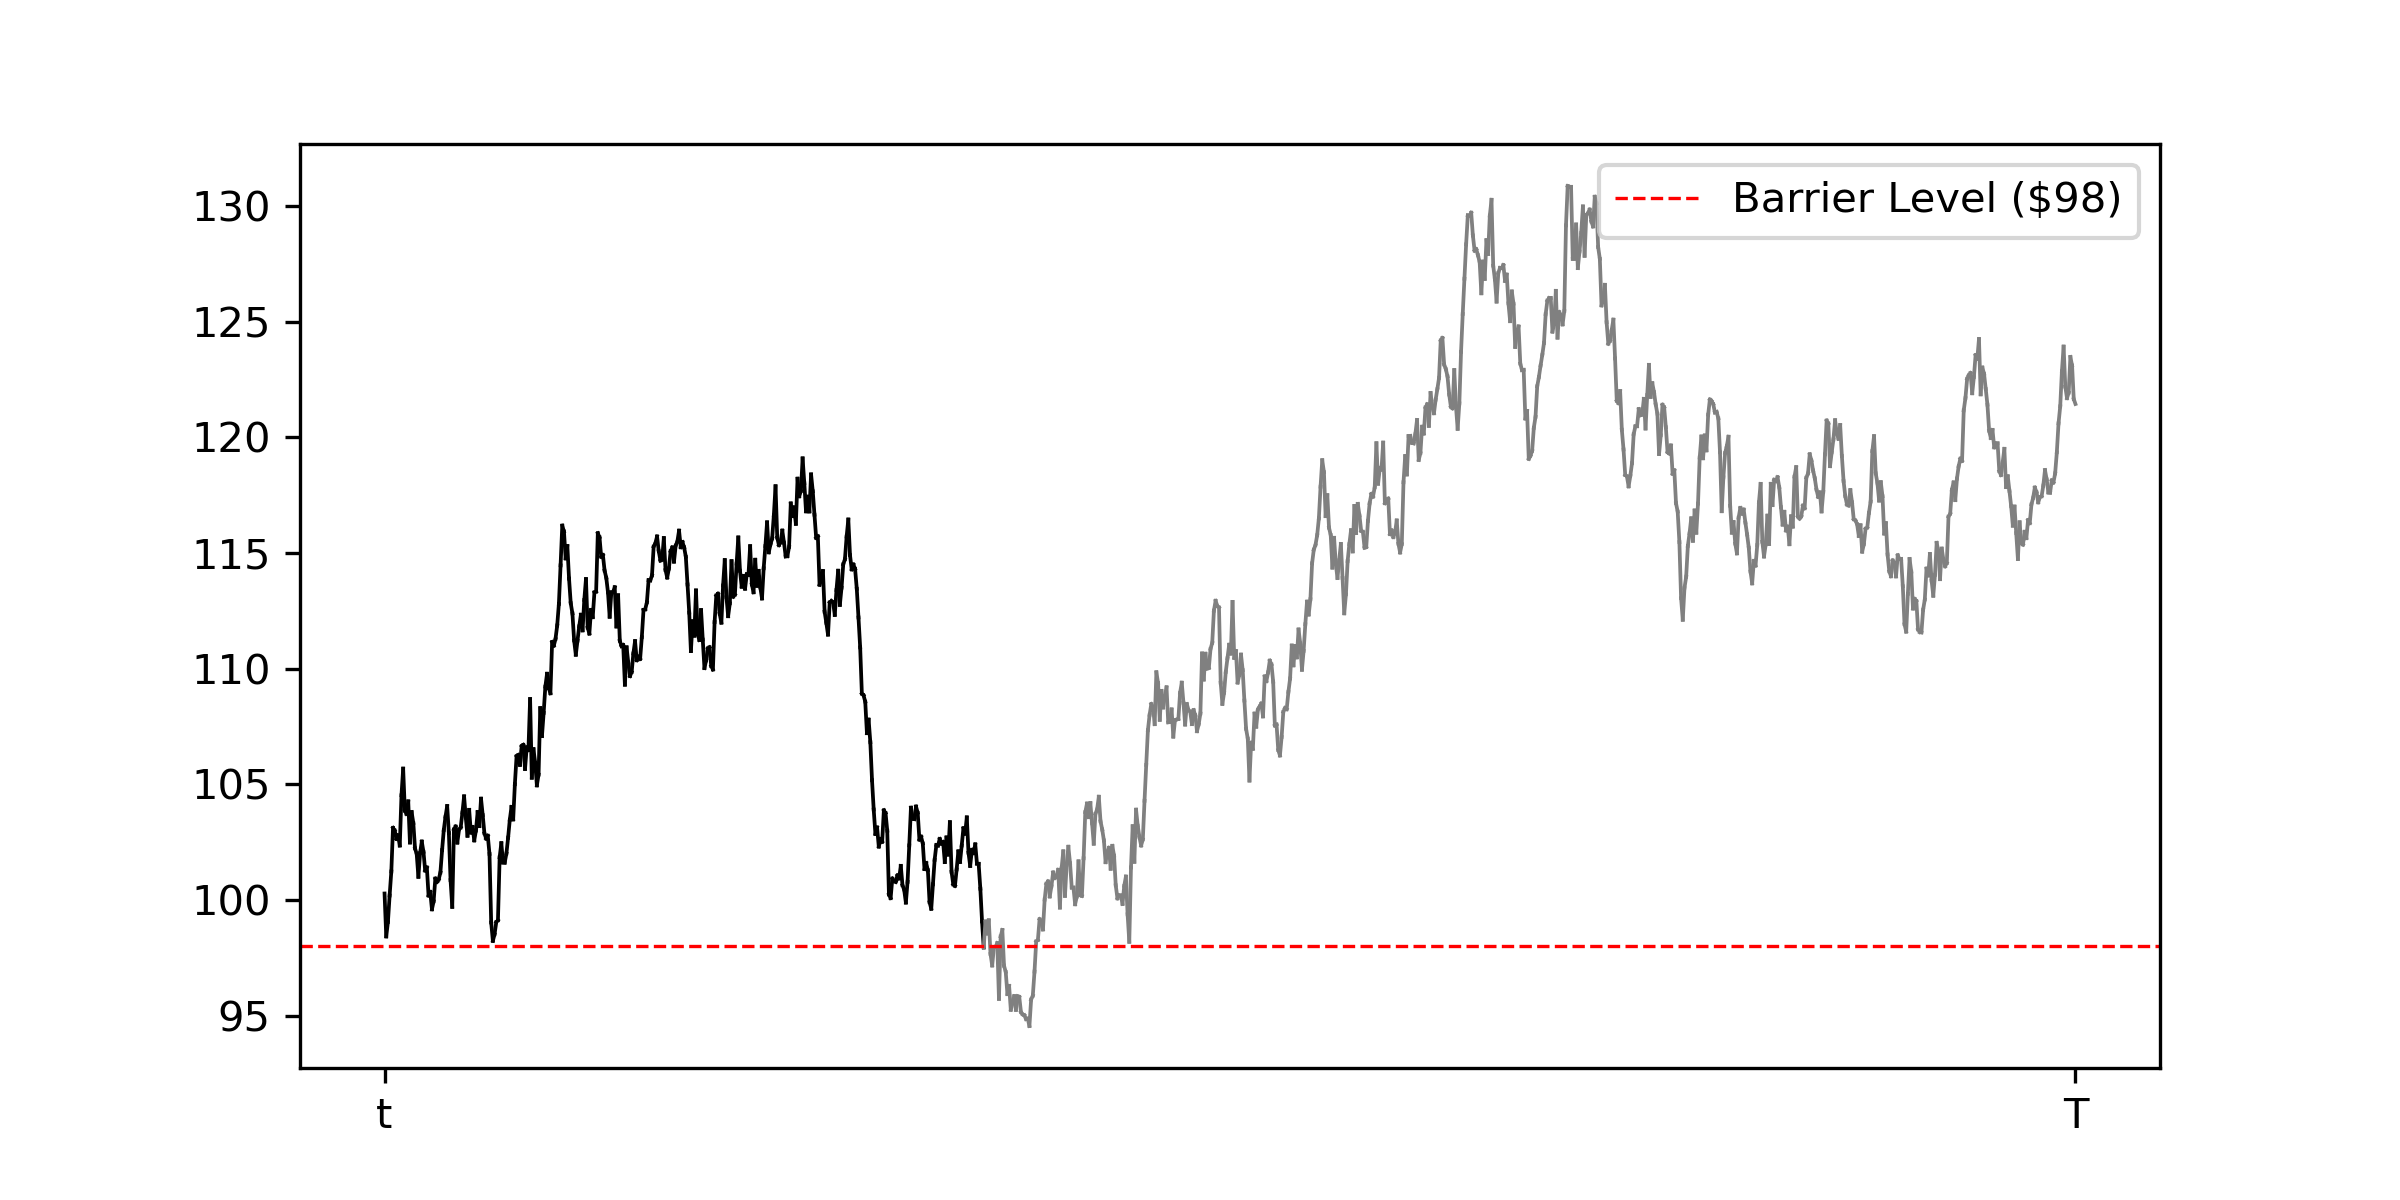
\includegraphics[width=\linewidth]{images/down_out_option.png}
      \caption{Down-and-Out Barrier Option}
      \label{fig:down_out_option}
    \end{subfigure}
    
    \caption{Illustration of Barrier Options: Displaying the active (black) and inactive (grey) phases of each option type. (a) Up-and-In Option, (b) Up-and-Out Option (c) Down-and-In Option, and (d) Down-and-Out Option. The red line represents the barrier.}
\end{figure}

The payoff depends on whether the price of the underlying asset reaches a certain level (the barrier) during the life of the option. A \textit{knock-in} barrier option only comes into existence if the barrier has been touched, while a \textit{knock-out} barrier option ceases to exist instead. For example, a \textit{down-and-out} barrier option (\autoref{fig:down_out_option}) is a type of knock-out option that becomes worthless if the price of the underlying asset falls below the barrier level. On the other hand, a \textit{down-and-in} barrier option (\autoref{fig:down_in_option}) is a type of knock-in option that only becomes active if the asset price falls below the barrier level.

\subsubsection{Double Barrier Options}\label{double_barrier}
Double barrier option involve two price levels: an upper and lower barrier that define the boundaries for the option's activity. These options can either be \textit{knock-in} or \textit{knock-out}. A double knock-in option becomes active only if the asset price hits either barrier, similar to a combination of \autoref{fig:up_in_option} and \autoref{fig:down_in_option}. Conversely, a double knock-out option ceases to exist if the asset price touches either barrier combining the characteristics of \autoref{fig:up_out_option} and \autoref{fig:down_out_option}.

% ========================================
% Modelling Asset Prices
% ========================================
\subsection{Modelling Asset Prices}
Accurate models allow traders, investors and risk managers to assess the fair value of financial products and make informed decisions. The Black-Scholes model assumes that the price of the underlying asset follows a geometric Brownian motion (GBM). Under this assumption, the asset price $S(t)$ evolves according to the stochastic differential equation:

\begin{equation}\label{black_scholes_equation}
dS(t) = \mu S(t) dt + \sigma S(t) dW(t),	
\end{equation}
where $\mu$ represents the expected return, and $W(t)$ is a standard Wiener process. The solution to this equation gives the asset price at time t as:

\begin{equation}
S(t) = S(0)e^{(\mu - 0.5 \sigma^2) + \sigma W(t)}	
\end{equation}

The model assumes that the volatility is constant, which is rarely the case as market volatility tends to fluctuate over time due to economics conditions or market sentiment. Additionally, the model doesn't account for jumps or sudden large movements in asset prices, usually seen at times of significant news. These limitations have led to the development of more sophisticated representations; given the scope and background of this project, we primarily focus on exponential L\'evy processes.

\subsubsection{Exponential L\'evy Processes}
We extend Eq. (\ref{black_scholes_equation}) by incorporating jump processes to account for sudden changes in asset prices. A stochastic process $X(t)$ is termed a L\'evy process if \textbf{(i)} the changes in the process are independent of each other, \textbf{(ii)} the distribution of the changes in the process depends only on the length of the time interval, not on the starting point, and \textbf{(iii)} it starts at zero, \textit{i.e.}, $X(0) = 0$. The dynamics of a L\'evy process can be described by the following stochastic differential equation:
\begin{equation}
dX(t) = \mu dt + \sigma dW(t) + dJ(t),
\end{equation}
where $J(t)$ represents a jump process (typically a compound Poisson process) to account for sudden, significant changes. An exponential L\'evy process describes the asset price process as:

\begin{equation}
S(t) = S(0)e^{X(t)}	
\end{equation}

As the characteristic function of exponential L\'evy models are often available in closed form, which facilitates the application of Fourier-based methods, they have been widely used in the pricing of path-dependent options as shown by the works of \citet{fusai2016spitzer, kwok2011efficient, feng2008pricing, phelan2019hilbert}.

% ========================================
% Fourier Based Pricing
% ========================================
\subsection{Fourier-Based Pricing}
The pricing of these options can be computationally expensive due to the high-dimensional integrals involved in the pricing formulas. Whilst \citet{heston1993closed} explored the idea of modelling asset prices in the Fourier domain, \citet{carr1999option} were the first to price European options expressing both the characteristic function and the payoff in the Fourier domain. It involved transforming the pricing problem from the time domain to the frequency domain, where the pricing formula simplifies to a one-dimensional integral. The Fourier-based methods have been widely used for the pricing of options discussed in Section \ref{section:discrete_monitoring} \citep{eberlein2010analysis}.

\citet{fang2009novel} introduced a pricing technique based on the Fourier-cosine expansion approximating the characteristic function of the underlying asset price, which was then expanded to a broader class of exotic options \citep{fang2009pricing, fang2011fourier} and general l\'evy processes \citep{lord2008fast}. Whilst the method shows high levels of accuracy with exponential error convergence on the number of terms, this is only the case when the governing probability density function is sufficiently smooth. When modelling the asset price by the variance gamma process \citep{madan1998variance}, we achieve only algebraic error convergence due to the discontinuities in the process. \citet{ruijter2015application} showed that this can be remedied using spectral filters however the issue remains in that the computational time is linearly dependent on the number of monitoring dates for discretely monitored options. This seems to also be the case for \citet{feng2008pricing}'s employment of the Hilbert transform using backward induction to price barrier options. 

In an effort to eliminate the computational inefficiency tied to the number of monitoring dates, \citet{fusai2006exact} looked into shifting the pricing problems from the time domain into the $z$-domain, where convolution operations become straightforward multiplications. This helped set the stage for \citet{fusai2016spitzer}'s method incorporating the Hilbert and $z$-transform to calculate the Wiener-Hopf factors, which decompose the characteristic function of the price process into two parts; positive and negative jumps. The authors demonstrated that the computational cost is independent of the number of monitoring dates, and the error decays exponentially with the number of grid points. Whilst extensions to the method have been made such as those by \citet{phelan2018fourier}'s new scheme using spectral filters to improve convergence \citep{phelan2019hilbert}, we shift our focus to the use-case of the inverse $z$-transform in the pricing of options.

% ========================================
% NIZT in Option Pricing
% ========================================
\subsection{NIZT in Option Pricing}
\todo[inline]{Need to solidify understanding}
We consider the case that of a double barrier option (Section \ref{double_barrier}), which are characterised by their dependency on the asset's price staying within a specified range between an upper boundary $u$ and a lower boundary $l$. The probability of the asset's price being at $x$ at the $n$th monitoring without hitting these barriers is represented by $f(x, n)$. This forms the basis of our recursive relationship for these options:

\begin{equation}
\int^u_l f(x', n-1)p(x - x', \triangle t)\ dx',	
\end{equation}
where $p(x - x', \triangle t)$ is the transition density between the states from $x'$ to $x$ over a small time increment $\triangle t$. The integral expression represents the transition probabilities convolved with the state probabilities from the previous time step, under the condition that the asset remains within the barriers $u$ and $l$. We expand this relationship across all monitoring periods as follows:

\begin{equation}
\sum^{\infty}_{n = 1} q^n f(x, n) = \sum^{\infty}_{n = 1} q^n \int^u_l f(x', n-1)p(x - x', \triangle t)\ dx'	
\end{equation}
We notice the similarity to that of Eq. (\ref{unilateral_z-transform}), however we set $z^{-1} = q$ to remain consistent with that in literature. By shifting the index $m = n-1$, the expression simplifies to
\begin{equation}
= q \int^u_l \sum^{\infty}_{m = 0} q^m f(x', m) p(x - x', \triangle t)\ dx'	
\end{equation}
This manipulation restructures the series into a form amenable to the use of transitioning to the $z$-domain. We define the $z$-transform of $f(x', n)$ as

\begin{equation}
\tilde{f}(x', q) = \mathcal{Z}_{n \rightarrow q}[f(x', n)] = \sum^{\infty}_{n = 0} q^nf(x', n)
\end{equation}
This encapsulation into $\tilde{f}(x', q)$ allows us to write the relationship as
\begin{equation}
\sum^{\infty}_{n = 0} q^n f(x, n) -q^0f(x, 0) = q\int^u_l \sum^{\infty}_{m = 0}q^m f(x', m) p(x-x', \triangle t)\ dx'	
\end{equation}
to which we can see how the $z$-transform helps in handling the summation over all $n$:
\begin{equation}
\tilde{f}(x', q) = q\int^u_l \tilde{f}(x', q)p(x - x', \triangle t)\ dx' + f(x, 0)
\end{equation}

Such a form enables the use of fourier-based methods; \citet{fusai2016spitzer} demonstrated that the iteration over all monitoring dates can be bypassed using the Spitzer identities, originally detailed by \citet{spitzer1957wiener} and expanded upon by \citet{kemperman1963wiener}. The identities require the Wiener-Hopf factorisations and decompositions, which were computed with the Plemelj-Sokhotsky relations and the Hilbert transform. Whilst \citet{fusai2016spitzer} provide a comprehensive list of references, we ought to also mention the continuations of \citet{phelan2018fluctuation, phelan2019hilbert, loveless2023phelanguido}. After such calculations, the inverse $z$-transform (Section \ref{section:inverse_z}) of $\tilde{f}(x, q)$ is needed to translate the representation back to the time-domain probabilities. Thus, the focus of this work on the inverse $z$-transform not only underscores its mathematical importance but also highlights its role in bridging theoretical constructs with real-world financial applications. 

% ========================================
% Experiment
% ========================================
\chapter{Experiment}
Having established the theoretical foundation, we now turn our attention to the practical implementation of methods proposed by \citet{AbateWhitt1992a, AbateWhitt1992b} and \citet{Cavers1978FFT}. Whilst the former is based on a circular contour, we also explore the idea laid out by \citet{levendorskii2022sinh} in sampling the $z$-transform on a sinh-deformation.

This chapter outlines the experimental setup, implementation and evaluation of the methods. We measure our results in terms of accuracy and computational efficiency against well-known transformation pairs (Table \ref{table:transform_pairs}) in an attempt to provide a thorough comparison of the methods.

All experiments were designed to be used on Visual Studio Code 1.89.1 using Python 3.11.7, NumPy 1.26.3 and MatPlotLib 3.8.0; we use such an environment given its robustness and extensive support for scientific computing and optimisation tasks. Whilst we outline all experiments/methods as pseudocode to allow for easy adaptations to other computing environments, the python implementation of the key functions are provided in Appendix (\ref{chapter:code_listings}).

% ========================================
% Transform Pairs
% ========================================
\section{Transform Pairs}
To measure the \textit{success} of our implementations, we find it convenient to use analytical transform pairs for the unilateral $z$-transform. Whilst a wide array of transform pairs exist, we focus on those listed in Table (\ref{table:transform_pairs}) as they are ``simple to compute and provide an excellent benchmark" for our use case \citep{loveless2021guido}. For each function $x(t)$, we derive the corresponding transform pair in the subsequent sections.

\begin{table}[H]
    \centering
    \renewcommand{\arraystretch}{1.2} % row height
    \begin{tabular}{c|cc}
    \textbf{Function} & $x(t)$ & $X(z)$ \\
    \hline
    Heaviside Step & 1 & $\frac{z}{z-1}$ \\
    Polynomial & $t$ & $\frac{z}{(z-1)^2}$ \\
    Decaying Exp & $e^{-at}$ & $\frac{z}{z - e^{-a \triangle t}}$ \\
    Sinusoidal & $\sin(\omega t)$ & $\frac{z^{-1}\sin(\omega \triangle t)}{1 - 2\cos(\omega\triangle t)z^{-1} + z^{-2}}$ \\
    \end{tabular}
    
    \caption{List of Transform Pairs}
    \label{table:transform_pairs}
\end{table}

% ========================================
% Heaviside Step
% ========================================
\subsection{Heaviside Step}\label{section:heaviside_step}
The Heaviside step function, $x(t)$, is an important piecewise function in signal processing and control theory \citep{proakis2007digital}. This is commonly defined as
\begin{equation}
	x(t) = 
	\begin{cases}
        0 & \text{if } t < 0 \\
        1 & \text{if } t \geq 0
    \end{cases}
\end{equation}

The unilateral $z$-transform of the Heaviside step function can be calculated using Eq. (\ref{unilateral_z-transform}):

\begin{equation}
X(z) = 	\mathcal{Z}_{t \rightarrow z}[x(t)] = \sum^{\infty}_{t = 0}x(t)z^{-t} = \sum^{\infty}_{t=0} z^{-t}
\end{equation}

We identify this as a geometric series where each term has the form $r^n$ with $r = z^{-1}$ and $n = t$. The sum of an infinite geometric series with first term $a$ and a common ratio $r$, where $|r| < 1$ is given by
\begin{equation}\label{equation:geometric_series}
S_\infty = \frac{a}{1-r}	
\end{equation}

For the sum to converge, we require $|z > 1|$ given the pole at $z = 1$, and it follows that

\begin{equation}
X(z) = \frac{1}{1 - z^{-1}} = \frac{z}{z - 1}
\end{equation}

% ========================================
% Polynomial
% ========================================
\subsection{Polynomial}
The polynomial function, often referred to as the linear ramp function, is defined as $x(t) = t$ for $t \geq 0	$. Following a similar approach to that of the previous section, we have

\begin{equation}
X(z) = 	\mathcal{Z}_{t \rightarrow z}[x(t)] = \sum^{\infty}_{t = 0}x(t)z^{-t} = \sum^{\infty}_{t=0} tz^{-t},
\end{equation}
in which we take note of the increasing integer multiplier $t$ and the kernel $z^{-t}$. To solve this series, we use the derivative property of the $z$-transform  given by

\begin{equation}
\mathcal{Z}_{t \rightarrow z}[tf(t)] = -z \frac{dF(z)}{dz},
\end{equation}
which shows that multiplying the sequence $f(t)$ by $t$ in the time domain corresponds to multiplying the z-transform $F(z)$ by $-z$ and taking the derivative with respect to $z$ in the z-domain. Thus, if we consider the Heaviside step function, it leads on that 

\begin{equation}
X(z) = -z \frac{d}{dz} \left( \frac{z}{z-1} \right) = -z \left( \frac{z - 1 - z}{(z-1)^2} \right) = \frac{z}{(z-1)^2}
\end{equation}

% ========================================
% Decaying Exponential
% ========================================
\subsection{Decaying Exponential}
The decaying exponential function, commonly expressed as $x(t) = e^{-at}$ for $t \geq 0$ and $a > 0$, is very useful in the analysis of systems with exponential decay or growth characteristics. However, such a signal is sampled at discrete time intervals; if $\triangle t$ is the sampling interval and $n$ represents the discrete time index, then the continuous function $x(t)$ becomes $x[n] = e^{-an\triangle t}$ when sampled at intervals of $\triangle t$. The unilateral $z$-transform of $x[n]$ is given by
\begin{equation}
	X(z) = 	\mathcal{Z}_{n \rightarrow z}[x[n]] = \sum^{\infty}_{n = 0}x[n]z^{-n} = \sum^{\infty}_{n=0} e^{-an\triangle t}z^{-n}
\end{equation}

This is a geometric series where each term is $(e^{-a\triangle t}z^{-1})^n$. Using Eq. (\ref{equation:geometric_series}), we can express $X(z)$ as:
\begin{equation}
X(z) = \frac{1}{1 - (e^{-a\triangle t}z^{-1})}= \frac{z}{(z-e^{-a\triangle t})}
\end{equation}

% ========================================
% Sinusoidal
% ========================================
\subsection{Sinusoidal}
The sinusoidal function $x(t) = \sin(\omega t)$ is a key waveform given its periodic nature. Similar to that of the decaying exponential transform pair, we discretely sample the function at intervals $\triangle t$, which results in the discrete time function $x[n] = \sin(\omega n \triangle t)$. Thus, the unilateral $z$-transform is computed as
\begin{equation}
X(z) = \mathcal{Z}_{n \rightarrow z}[x[n]] = \sum^{\infty}_{n = 0}x[n]z^{-n} = \sum^{\infty}_{n = 0} \sin(\omega n \triangle t)z^{-n}
\end{equation}

We make use of Euler's formula, defined as $\sin(x) = \frac{e^{ix} - e^{-ix}}{2i}$, to express our sine function and split the term into two separate geometric series:
\begin{equation}
	X(z) = \sum^{\infty}_{n = 0} \left( \frac{e^{i\omega n\triangle t} - e^{-i\omega n\triangle t}}{2i} \right) z^{-n} = \frac{1}{2i}\cdot\left( \sum^{\infty}_{n = 0} e^{i\omega n\triangle t} z^{-n} - \sum^{\infty}_{n = 0} e^{-i\omega n\triangle t}z^{-n}\right)
\end{equation}
 
 We then refer back to Eq. (\ref{equation:geometric_series}) to express the summations as functions of $z$. It follows on that
\begin{equation}
	X(z) = \frac{1}{2i}\cdot \left( \frac{1}{1 - e^{i\omega \triangle t}z^{-1}} - \frac{1}{1 - e^{-i\omega \triangle t}z^{-1}} \right)
\end{equation}
where we simplify it into the form:
\begin{equation}
X(z) = \frac{1}{2i} \cdot \frac{ -z^{-1}(e^{i\omega \triangle t} - e^{i\omega \triangle t})}{(1 - e^{i\omega \triangle t}z^{-1})(1 - e^{-i\omega \triangle t}z^{-1})} = \frac{z^{-1}\sin(\omega \triangle t)}{1 - 2\cos(\omega\triangle t)z^{-1} + z^{-2}}
\end{equation}

% ========================================
% Circular Contour
% ========================================
\section{Circular Contour}\label{section:circular_contour}
``The inverse at point $T$ can be obtained from the contour integral where $C$ is a counter-clockwise closed path encircling the origin and entirely in the region of convergence'' \citep{horvath2020numerical}. A circular contour is commonly used to solve Eq. (\ref{inverse_z-transform}), defined as $z = re^{i\theta}$, however the setting of $r$ is important as shown for Example (\ref{example:roc_poles}) in Figure (\ref{fig:effect_r}).

We thus formulate an algorithmic approach to the implementations of the NIZT outlined in Section (\ref{section:abate_whitt}) and Section (\ref{section:cavers}). For each of the methods, we outline a series of experiments and validation tests to carry out.

\begin{figure}[H]
    \begin{subfigure}{.25\linewidth}
      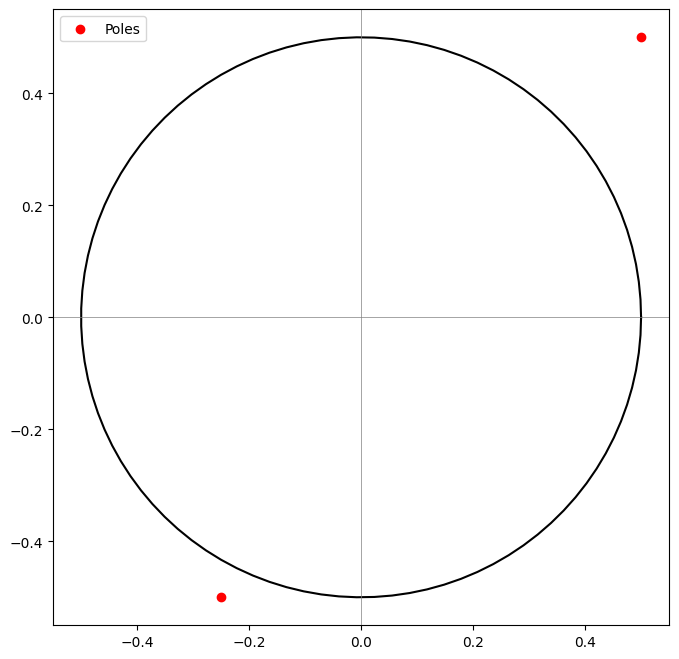
\includegraphics[width=\linewidth]{images/invalid_contour.png}
      \caption{r = 0.5}
    \end{subfigure}\hfill
    \begin{subfigure}{.25\linewidth}
      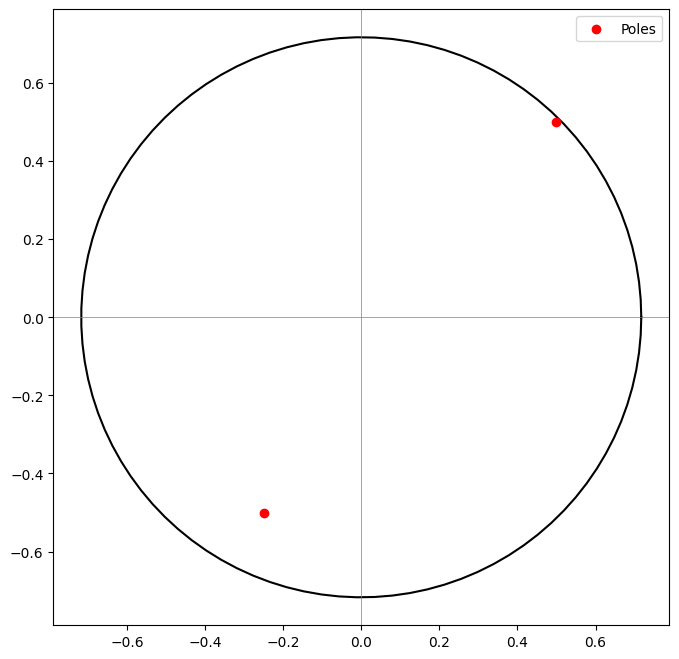
\includegraphics[width=\linewidth]{images/valid_border_contour.png}
      \caption{r = 0.72 (2 d.p.)}
      \label{fig:valid_r}
    \end{subfigure}\hfill
    \begin{subfigure}{.25\linewidth}
      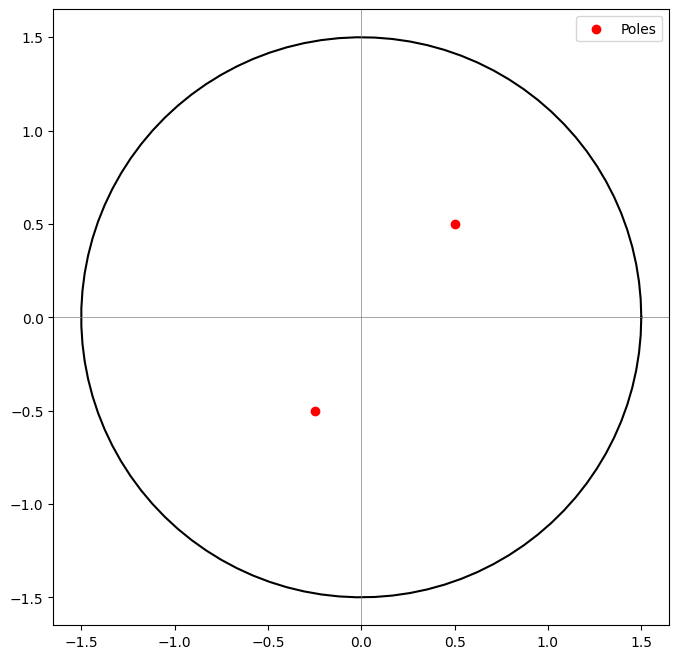
\includegraphics[width=\linewidth]{images/unstable_contour.png}
      \caption{r = 1.5}
    \end{subfigure}\hfill
    
    \caption{ Displaying the effect of the radius $r$ on a circular contour ($n = 100$). The red dots represent the poles of $H(z)$ in Example (\ref{example:roc_poles}) with (a) including the poles within the ROC, (b) excluding the poles but inclusive of the unit circle, and (c) excluding the poles but not stable.}
    \label{fig:effect_r}
\end{figure}

% ========================================
% Abate and Whitt 1992
% ========================================
\subsection{Abate and Whitt 1992}
Given a sufficient hyperparameter setup, we will require, as input,  just the function to be inverted, $\tilde{f}: \mathbb{C}\rightarrow \mathbb{C}$, and the point $n_\in \mathbb{R}$. The implementation of such a function follows very easily from Eq. (\ref{eq:aw_inversion}) as shown in the pseudocode below:

\begin{algorithm}[H]
    \caption{Implementation of Equation \ref{eq:aw_inversion}}
    \label{algo:abate_whitt}
    \begin{algorithmic}[1]
    \Procedure{AbateWhitt}{$\tilde{f}, n$}
        \State $\lambda \gets \mathbb{R}^+$
        \State $r \gets 10^{-\lambda / (2 \cdot n)}$
        \State $\text{summation} \gets 0$
        \For{$k \gets 1$ \textbf{to} $n$}
            \State $z \gets \frac{1}{r \cdot \exp(\text{i} \cdot k \cdot \pi / n)}$
            \State $\text{sum} \gets \text{sum} + (-1)^k \cdot \text{Re}(\tilde{f}(z))$
        \EndFor
        \State $\text{sum} \gets \tilde{f}(\frac{1}{r}) + 2 \cdot \text{sum} + (-1)^n \cdot \tilde{f}(-\frac{1}{r})$
        \State \Return $\frac{\text{sum}}{2 \cdot n \cdot r^n}$
    \EndProcedure
    \end{algorithmic}
\end{algorithm}

\subsubsection{Computational Accuracy}
\citet{AbateWhitt1992a, AbateWhitt1992b} showed that the absolute error, $|\epsilon |$, of their implementation is bounded by
\begin{equation}
	| \epsilon | = \frac{1}{r^N - 1} \approx \frac{1}{r^N},
\end{equation}
where the approximation holds for large $r^N$. As discussed in Section (\ref{section:abate_whitt}), setting $r=10^{-\lambda / 2n}$  yields an accuracy of $10^{-\lambda}$, \textit{i.e.}, $\lambda$ significant digits. However, we have that if the machine accuracy is $\epsilon_m = 10^{-\lambda_m}$, the bound falls apart around $\lambda > \frac{2}{3} \lambda_m$ \citep[Remark 5.8]{AbateWhitt1992a}. \citet{loveless2023phelanguido} states that ``with IEEE 754 double precision representation of floating point numbers, $\epsilon_m = 2^{-52} \approx 10^{-15.65}$, and thus it makes little sense to set $\lambda > 10.5$, which yields the IZT up to about 10 or 11 significant digits".

Thus, we investigate the effect of different values of $\lambda$ on the accuracy of the Abate-Whitt method when applied to the Heaviside step and polynomial transform pairs (Table \ref{table:transform_pairs}). We expect to observe an increase in accuracy as $\lambda$ increases, up to a certain point where the limitations of machine precision and rounding errors become dominant.

\subsubsection{Computational Speed}\label{section:aw_speed}
In addition to accuracy, computational efficiency is another important factor to consider. The Abate-Whitt algorithm described in Section (\ref{section:abate_whitt}) has a time complexity of O($n$), where $n$ is the number of terms used in the approximation. This is evident in Algorithm (\ref{algo:abate_whitt}) for the inclusion of the single for loop. With each iteration, the dominant operations is the evaluation of the input function $\tilde{f}$. Assuming the function evaluation time is bounded by some constant, the overall time complex remains O($n$). 

We thus run tests to empirically verify this linear complexity. Plotting the computation time against $n$ should show an approximately linear relationship if the O($n$) analysis holds in practice. Practically, it is not feasible to eliminate any interference from external background processes. However, we make efforts to minimise such effects by executing multiple runs of each test and taking the average.

% ========================================
% Cavers 1978
% ========================================
\subsection{Cavers 1978}
As discussed in Section (\ref{section:cavers}), \citet{Cavers1978FFT} introduces a secondary grid defined by the parameter $N_\in \mathbb{R}^+$ and it follows on that our algorithm will require this as input. We also remind ourselves that the methods differs in regard to the type of $n$; the data type is a list of integers compared to the previously mentioned where we passed an integer. The implementation is presented as:

\begin{algorithm}[H]
    \caption{Implementation of \autoref{cavers}}
    \label{algo:cavers}
    \begin{algorithmic}[1]
        \Procedure{Cavers}{$\tilde{f}, n, N$}
        	\State $\gamma \gets \mathbb{R}^+$
            \State $r \gets 10^{\gamma / N}$
            \State $z \gets \text{Array}[N]$
            \For{$k \gets 0$ \textbf{to} $N-1$}
                \State $z[k] \gets r \cdot \exp(\text{i} * 2 \pi * k / N)$
            \EndFor
            \State $F \gets \text{Array}[N]$
            \State $F \gets \text{IFFT}(\tilde{f}(z))$
            \State $f \gets r^n \cdot F[n]$
            \State \Return $f$ 
        \EndProcedure
    \end{algorithmic}
\end{algorithm}

Whilst the latter makes use of the IFFT, we look into analysing the comparative metrics with the definition including that of the numerical approximation given by Eq (\ref{equation:cavers_sum}). We denote the the number of points in the secondary grid as $J$ and let $N$ be the last value / length of $n$.

\begin{algorithm}[H]
\caption{Implementation of \autoref{equation:cavers_sum}}
\label{algo:cavers_sum}
\begin{algorithmic}[1]
\Procedure{Cavers\_sum}{$\tilde{f}, n, J$}
	\State $\gamma \gets \mathbb{R}^+$
	\State $N = n[-1]$
    \State $r \gets 10^{\gamma / J}$ 
    \State $z \gets \text{Array}[J]$
    \For{$j \gets 0$ \textbf{to} $J$}
                \State $z[j] \gets r \cdot \exp{(i * 2\pi * j / N)}$
            \EndFor
    \State $f \gets \text{Array}[N]$
    \For{$i \gets 0$ \textbf{to} $N$}
        \State $f[i] \gets \frac{1}{J} \cdot \sum (z^{n[i]} \cdot \tilde{f}(z))$ 
    \EndFor
    \State \textbf{return} $f$
\EndProcedure
\end{algorithmic}
\end{algorithm}

\subsubsection{Computational Accuracy}
As discussed in Section (\ref{section:cavers}), achieving machine-level accuracy is possible but requires some optimisation of the hyper-parameters. We aim to view the accuracy in regard to changes of the hyper-parameter $n$, $N$ and the setting of $\gamma$. In an attempt to ``exploit as much as possible the available digits of precision", \citet{loveless2023phelanguido} look into setting $\gamma = J\log_{10}(2)$. Thus, we aim to investigate the changes of the hyper-parameters on the accuracy as well as finding the implementation that achieves the best result for each transform pair in Table (\ref{table:transform_pairs}).

\subsubsection{Computational Speed}
For consistency, we plot the results against different N values, similar to our experiment for Section (\ref{section:aw_speed}), where we set J = 2N, for the different implementations. Given that IFFT has a time complexity of O(NLogN), we expect this to be the dominating factor in Algorithm (\ref{algo:cavers}). The numerical summation method, outlined in Algorithm (\ref{algo:cavers_sum}), requires computing the summation over J terms for each of the N terms. Thus, we expect a linear relationship with respect to NJ.

Similar to the approach in Section (\ref{section:aw_speed}), we take the average over multiple runs to minimise the interference of external processes.

\subsection{Comparative Analysis}

% ========================================
% Sinh Deformation
% ========================================
\section{Sinh Deformation}\label{section:sinh_deformation}
A circular contour integral is commonly used for approximating the inverse $z$-transform as we've seen in Section (\ref{section:abate_whitt}) and (\ref{section:cavers}). However, this does not mean it may be the best option. \citet{levendorskii2022sinh} propose a new method for a numerical evaluation of Eq. (\ref{inverse_z-transform}) by deforming the commonly used circular contour $\{z = re^{i\theta} | -\pi < \theta < +\pi\}$ through the conformal mapping:
\begin{equation}\label{equation:conformal_mapping}
    \xi(y) = \sigma + ib\sinh(i\theta + y),
\end{equation}
where parameters are chosen such that $\sigma,y_\in \mathbb{R}$, $b_\in \mathbb{R}^+$, and $\theta$ is restricted to the interval $(-\pi/2, \pi / 2)$. The unique selection of parameters allows the contour to be tailored specifically to the characteristics of $X(z)$. The authors state that the conformal mapping alleviates typical errors which are discussed in the relevant texts \citep{boyarchenko2014efficient, boyarchenko2019sinh, schmelzer2007computing}. \todo{to look at these "typical" errors} Applying a change of variables to Eq. (\ref{inverse_z-transform}) yields

\begin{equation}
    x(n) = \int_\mathbb{R} \frac{b}{2\pi} \xi(y)^{-n-1} \cosh(i\theta + y) X(\xi(y)) dy.
\end{equation}

By denoting the integrand as $f_n(y)$ and approximating the application of the infinite trapezoidal, we have 
\begin{equation}
    x(n) \approx 2 \epsilon\ \text{Re}\left( \sum_{j = 0}^{M_0} f_n(j \epsilon)(1 - \delta_{j0}/2) \right)
\end{equation}

\todo[inline]{need to look more into it}

\begin{itemize}
    \item mention sufficient conditions under which this works (next paper)
    \item talk about why he does this
    \item our experiment in trying to recreate the unit circle and why
\end{itemize}

% ========================================
% Deforming the Contour
% ========================================
\subsection{Deforming the Contour}\label{section:deforming_contour}
In an attempt to recreate the unit circle from the conformal mapping (\autoref{equation:conformal_mapping}), we first try to understand the effects of the parameters on the contour.  We plot the contour for different values of $\sigma, b$ and $y$ to observe the deformation.

\begin{algorithm}[H]
\caption{Implementation of \autoref{equation:conformal_mapping}}
\label{algo:hyperbolic_sine}
\begin{algorithmic}[1]
\Procedure{Hyperbolic\_sine}{$\sigma, b, y, N$}
    \State $z \gets \text{Array}[N]$ \Comment{$z_{\in} \mathbb{C}^N$}
    \For{$k \gets -\frac{N}{2}$ \textbf{to} $\frac{N}{2}$}
        \State $\omega \gets \frac{i\pi  k}{N}$
        \State $z[k + \frac{n}{2}] \gets \sigma + i * b * \sinh(\omega + y)$
    \EndFor
    \State \textbf{return} $z$
\EndProcedure
\end{algorithmic}
\end{algorithm}

\begin{figure}[H]
    \begin{subfigure}{.3\linewidth}
      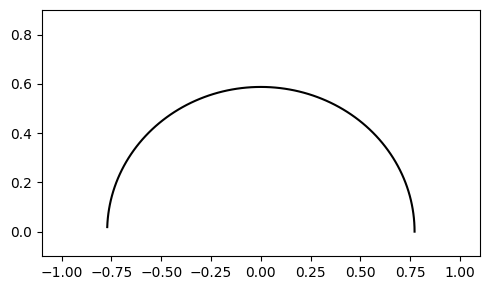
\includegraphics[width=\linewidth]{images/deformations/base.png}
      \caption{$\sigma = 0, b = 0.5, y = 1.0$}
      \label{fig:base_deform}
    \end{subfigure}\hfill
    \begin{subfigure}{.3\linewidth}
      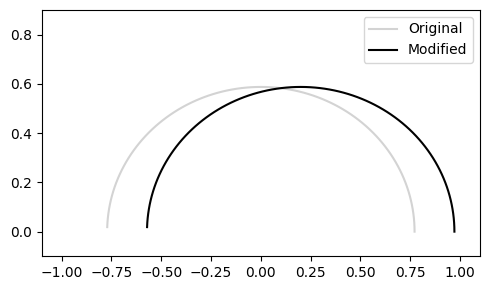
\includegraphics[width=\linewidth]{images/deformations/positive_sigma.png}
      \caption{$\sigma + 0.2$}
      \label{fig:positive_sigma}
    \end{subfigure}\hfill
    \begin{subfigure}{.3\linewidth}
      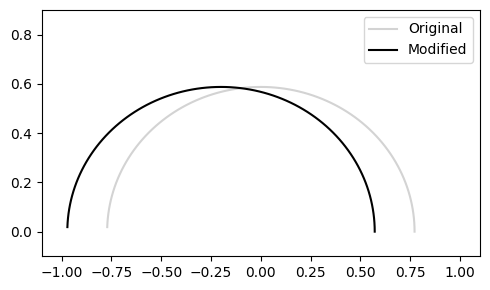
\includegraphics[width=\linewidth]{images/deformations/negative_sigma.png}
      \caption{$\sigma - 0.2$}
        \label{fig:negative_sigma}
    \end{subfigure}

    \medskip

    \begin{subfigure}{.3\linewidth}
        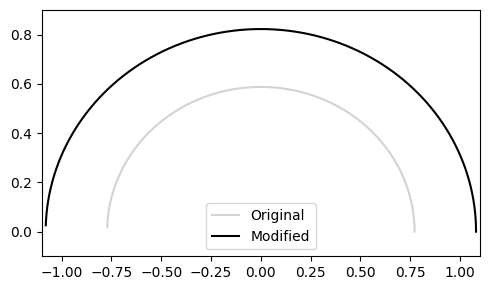
\includegraphics[width=\linewidth]{images/deformations/higher_b.png}
        \caption{$b + 0.2$}
        \label{fig:higher_b}
      \end{subfigure}\hfill
      \begin{subfigure}{.3\linewidth}
        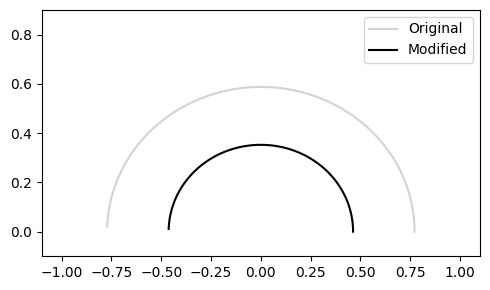
\includegraphics[width=\linewidth]{images/deformations/lower_b.png}
        \caption{$b - 0.2$}
        \label{fig:lower_b}
      \end{subfigure}\hfill
      \begin{subfigure}{.3\linewidth}
        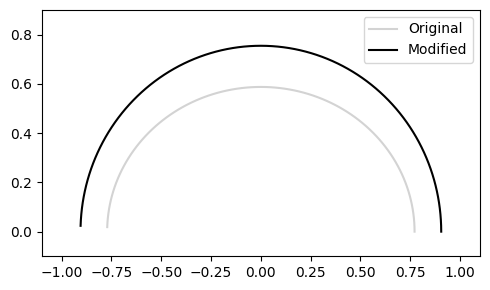
\includegraphics[width=\linewidth]{images/deformations/higher_y.png}
        \caption{$y + 0.2$}
        \label{fig:higher_y}
      \end{subfigure}

      \medskip

    \begin{subfigure}{.3\linewidth}
        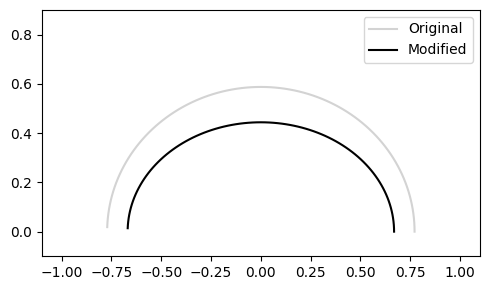
\includegraphics[width=\linewidth]{images/deformations/lower_y.png}
        \caption{$y - 0.2$}
        \label{fig:lower_y}
      \end{subfigure}\hfill
      \begin{subfigure}{.3\linewidth}
        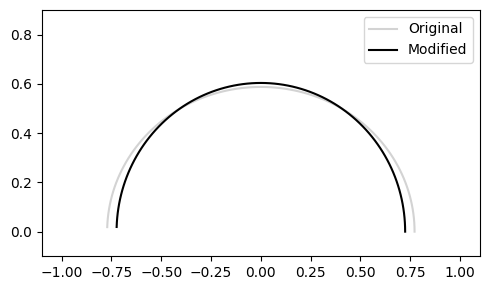
\includegraphics[width=\linewidth]{images/deformations/mixing_b_y.png}
        \caption{$b - 0.1, y + 0.2$}
        \label{fig:mixing_b_y}
      \end{subfigure}\hfill
      \begin{subfigure}{.3\linewidth}
        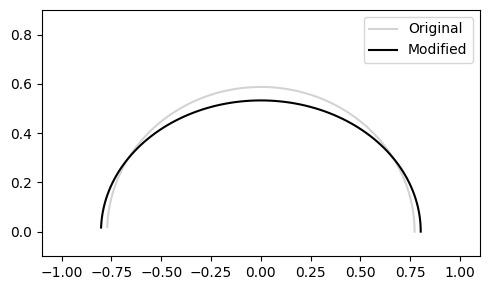
\includegraphics[width=\linewidth]{images/deformations/mixing_b_y_v2.png}
        \caption{$b + 0.1, y - 0.2$}
        \label{fig:mixing_b_y_v2}
      \end{subfigure}
    
    \caption{Displaying the effect of the parameters on the contour for Algorithm (\ref{algo:hyperbolic_sine}) with $\{-\frac{\pi}{2} \leq \theta \leq \frac{\pi}{2} \}$ and $n = 100$ points. Plots (b, c, d, e, f, g, h, i) highlights the changes in parameter the effects on the contour in comparison to the base contour (a). The black line represents the created contour, with the grey contour representing the base contour with parameters $\sigma = 0, b = 0.5, y = 1.0$.}
    \label{fig:deforming_all}
\end{figure}

In relation to the base contour (\autoref{fig:base_deform}), we observe that increasing $\sigma$ shifts the contour to the right (\autoref{fig:positive_sigma}), while decreasing $\sigma$ shifts the contour to the left (\autoref{fig:negative_sigma}). The parameter $b$ acts as a scale factor on the sinh deformation as shown in \autoref{fig:higher_b} and \ref{fig:lower_b}. Similarly, $y$ acts as a scale factor but with a more pronounced vertical effect as seen in \autoref{fig:higher_y} and \ref{fig:lower_y}. Mixing the parameters $b$ and $y$ results in a more complex deformation where the counter-opposing effects changes the contour in a non-linear manner (\autoref{fig:mixing_b_y} and \ref{fig:mixing_b_y_v2}).

\begin{figure}[H]
    \begin{subfigure}{.3\linewidth}
      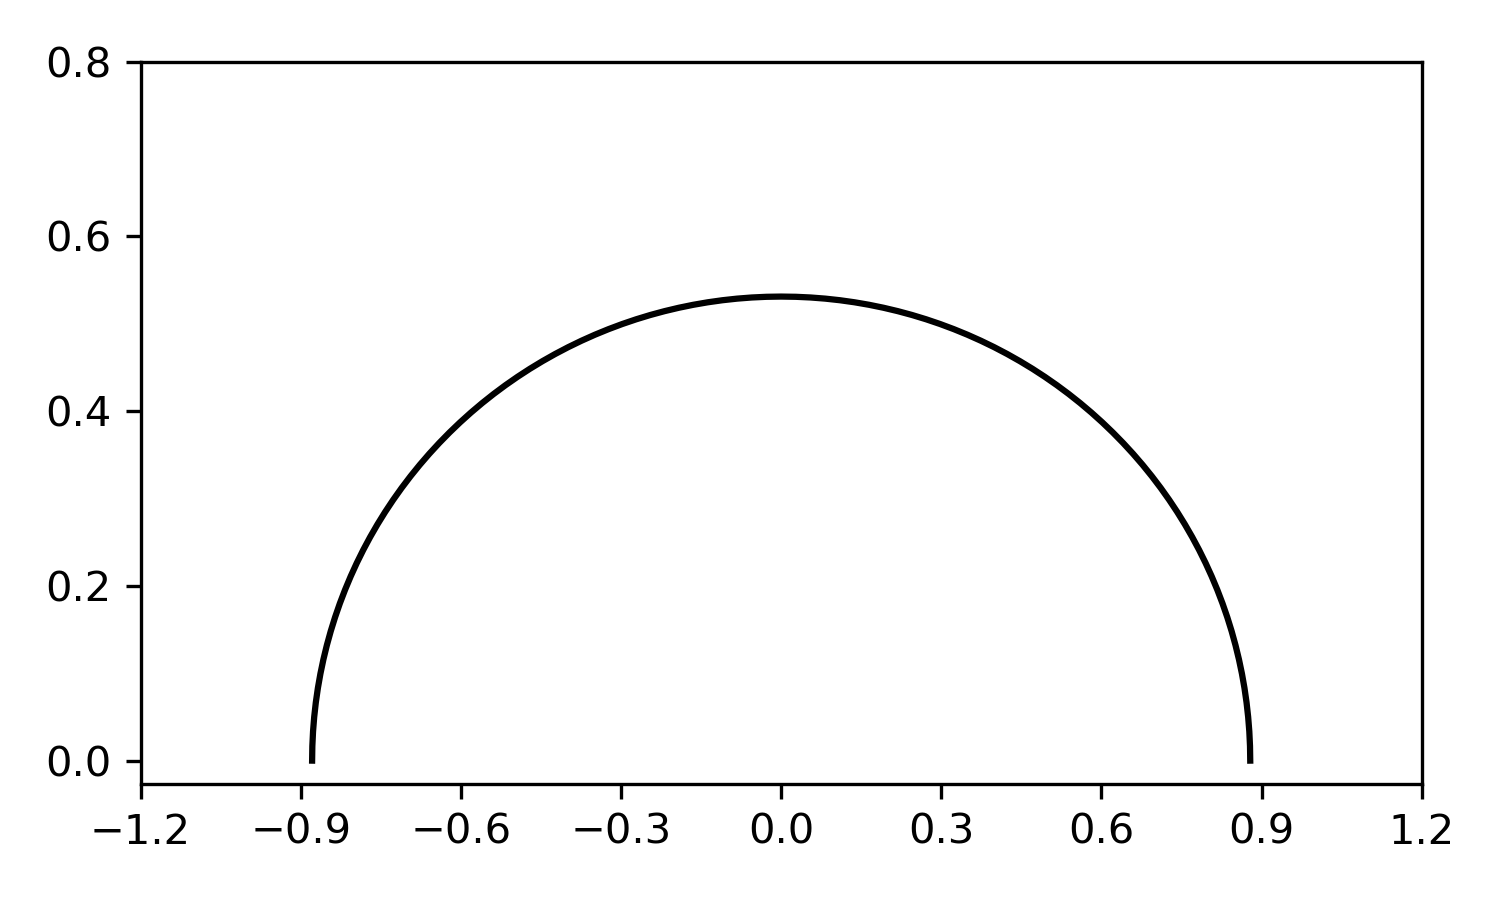
\includegraphics[width=\linewidth]{images/sinh_param_analysis/sinh_0_88.png}
      \caption{$\text{max(Re}(z)) = 0.88$ (2 d.p.)}
      \label{fig:extent_default}
    \end{subfigure}\hfill
    \begin{subfigure}{.3\linewidth}
      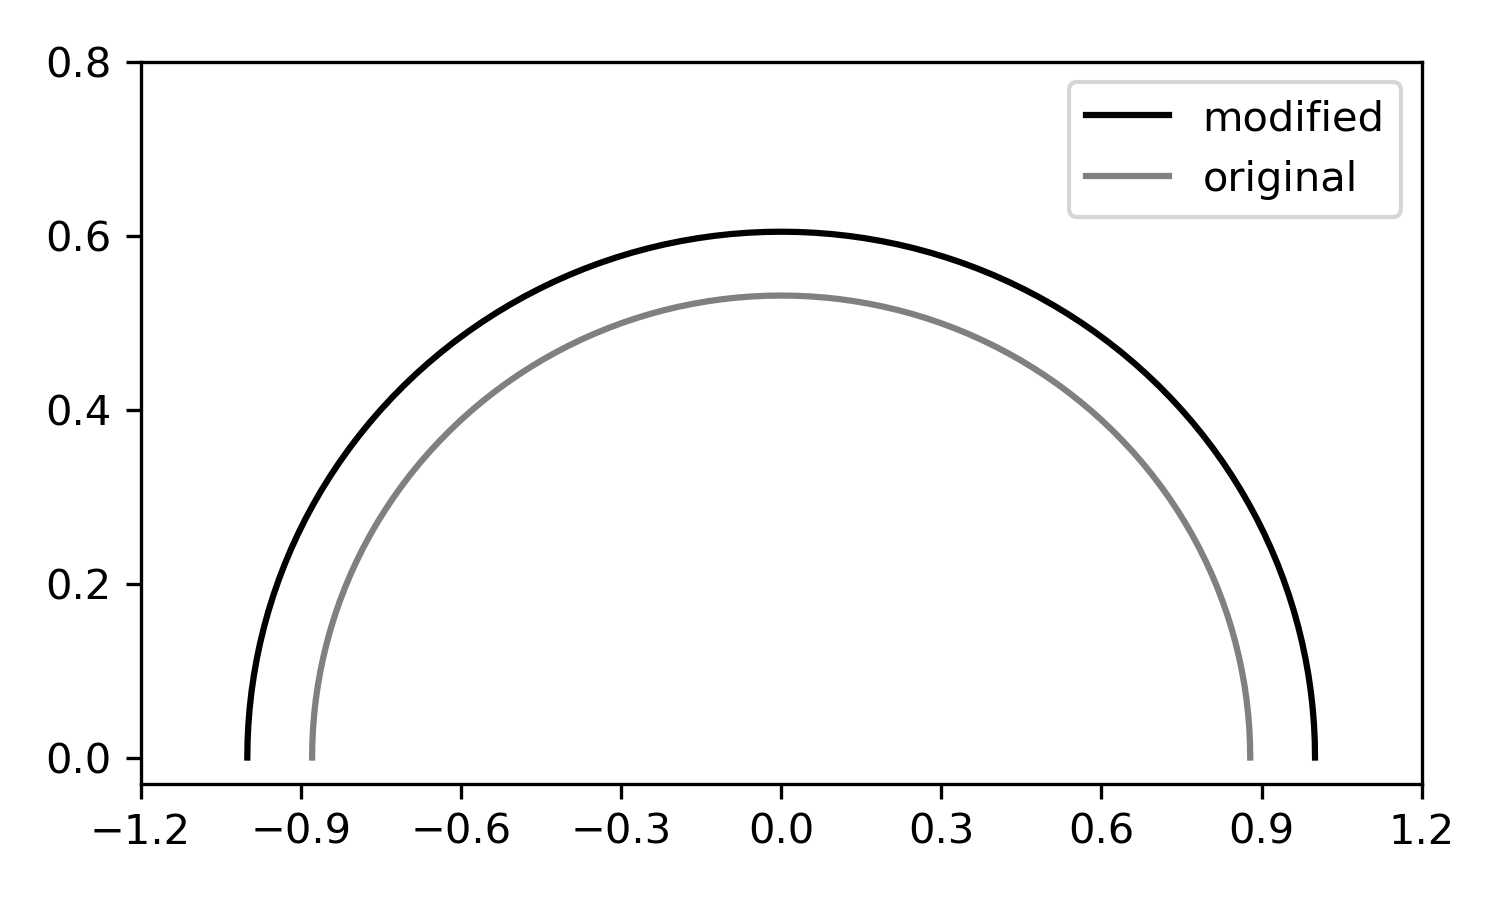
\includegraphics[width=\linewidth]{images/sinh_param_analysis/sinh_1_b.png}
      \caption{$\text{max(Re}(z)) = 1.0$ }
      \label{fig:extent_b}
    \end{subfigure}\hfill
    \begin{subfigure}{.3\linewidth}
      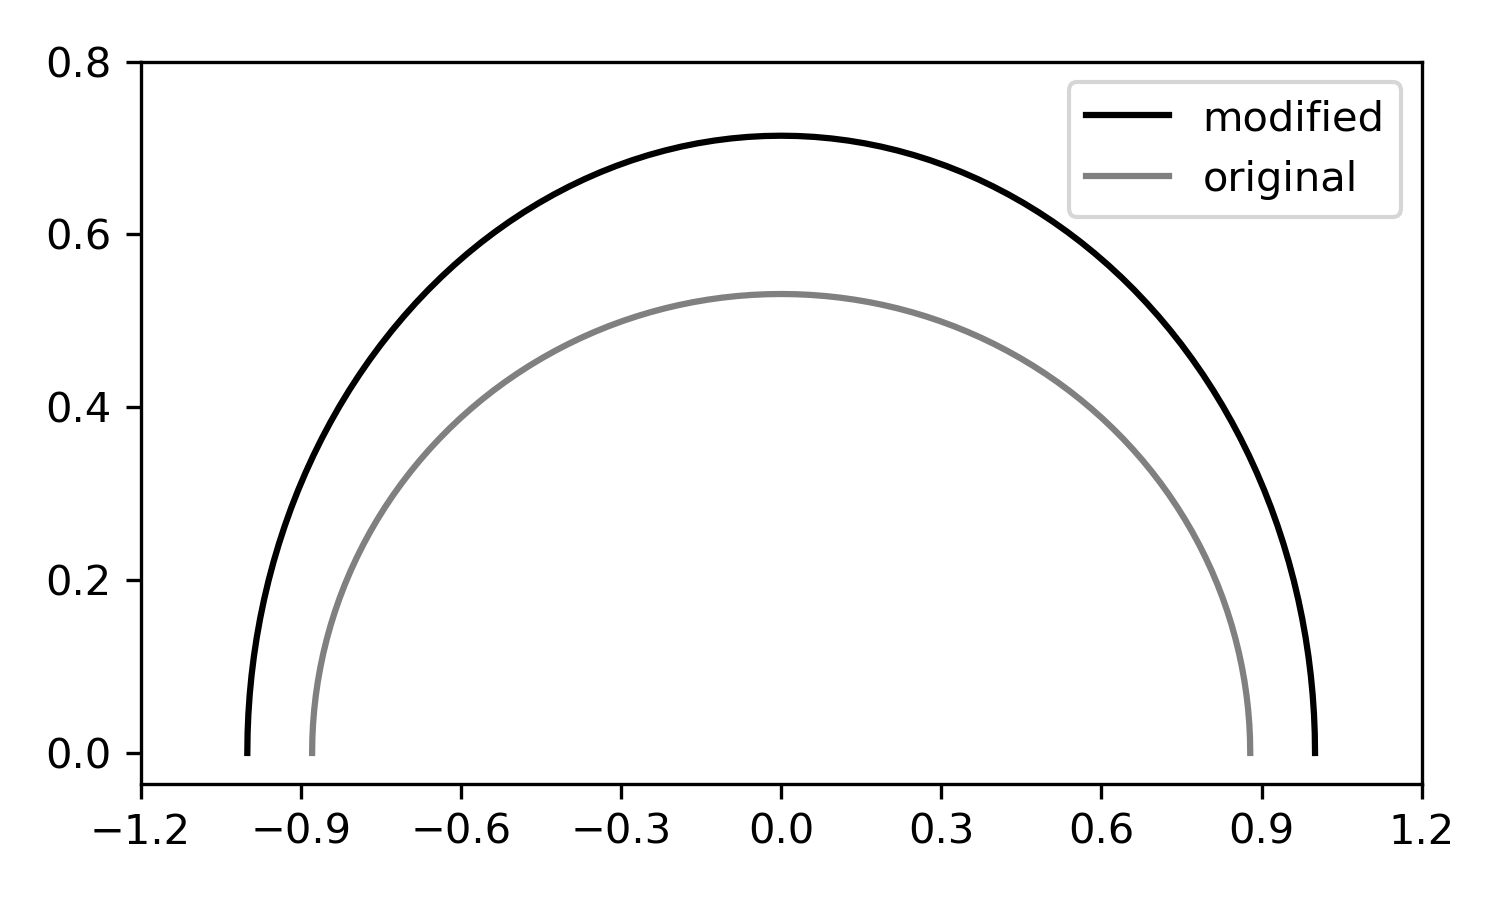
\includegraphics[width=\linewidth]{images/sinh_param_analysis/sinh_1_y.png}
      \caption{$\text{max(Re}(z)) = 1.0$}
      \label{fig:extent_y}
    \end{subfigure}
    
    \caption{Displaying the scaling effect of parameters $b$ and $y$. The initial deformation is created with \textbf{(a)} $\sigma = 0.0, b = 0.7, y = 0.7$ and the scaled results are constructed with \textbf{(b)} setting only $b = 0.7967054596179172$ and \textbf{(c)} setting only $y = 0.895588098866514$. The parameters were constructed with N = 100 points and chosen with an error tolerance of E-9.}
\end{figure}

To achieve an extent on the real axis of 1.0, we scale our original deformation (\autoref{fig:extent_default}) by the individual parameters. We see the differences in transformation in Figure (\ref{fig:extent_b}) and Figure (\ref{fig:extent_y}) for parameters $b$ and $y$, respectively.

% ========================================
% Parameter Selection for the Sinh Deformation
% ========================================
\subsection{Parameter Selection for the Sinh Deformation}\label{section:parameter_selection}
Given the complex changes resulting from the parameters $b$ and $y$, we utilise optimisation techniques (Section \ref{section:optimisation_techniques}) to find values that yield a contour resembling the unit circle. To achieve this, we first formulate a loss function, $L_1$, to set out our criteria. We let 
\begin{equation*}
	z = [z_0, z_1, .., z_{n-1}]
\end{equation*}
be the representation of a contour consisting of $|z| = n$ points, where $z_k = x + iy$ for $0 \leq k < n$. If we consider the unit circle, each point $z_k$ has a distance of $1$ from the origin (0,0). Thus, to compare the similarity for a given contour, we can define the loss function $L_1: \mathbb{C}^n \rightarrow \mathbb{R}$ as:
\begin{equation}
L_1 = \sum_{i=0}^{n-1} \left( |z_i| - 1 \right)^2,
\end{equation}
where we square the deviation of each point $z_i$ from that of the unit radius to account for both positive and negative differences. The summation of all the squared deviations gives us our total loss. As a comparative measure, we compute the loss for the upper half of the unit circle for $n = 100$ points and $\theta_\in [0, \pi]$: $L_1\approx$ 7E-31.

To minimise $L_1$ for a given contour, we initially use the gradient descent algorithm outlined in Algorithm (\ref{algo:gradient_descent}). We numerically estimate the partial derivative of $L_1$, with respect to $x$, using finite difference approximation with $\epsilon = 10^{-8}$; consult \citep{burden1997numerical}:
\begin{equation}\label{eq:finite_diff}
\frac{\partial L_1}{\partial x} \approx \frac{L_1(x + \epsilon) - L_1(x)}{\epsilon}
\end{equation}

From our understanding of the parameter $\sigma$, seen in Section (\ref{section:deforming_contour}), we set it to 0 and try to learn the parameters $b$ and $y$. The general steps is given by:

\begin{algorithm}[H]
\caption{GD for Minimising \( L_1 \)}
\label{algo:gd_l1}
\begin{algorithmic}[1]
\Procedure{GD}{$\alpha, \ell$}
    \State Initialise $b$ and $y$ \Comment with given constraints (Section \ref{section:sinh_deformation})
    \State $\sigma \gets 0.0$
    \State $n \gets 100$
    \State $L_1 \gets \infty$
    \While {$L_1 < \ell$} \Comment until loss within acceptable tolerance 
        \State $z \gets \texttt{hyperbolic\_sine}(\sigma, b, y, n)$ \Comment outlined in Algorithm (\ref{algo:hyperbolic_sine})
        \State $L_1 \gets \sum_{i=0}^{|z|} (|z2_i| - 1)^2$
        \State Compute gradients $\frac{\partial L_1}{\partial b}$ and $\frac{\partial L_1}{\partial y}$
        \State $b \gets b - \alpha \frac{\partial L_1}{\partial b}$
        \State $y \gets y - \alpha \frac{\partial L_1}{\partial y}$
    \EndWhile
    \State \textbf{return} $b, y$
\EndProcedure
\end{algorithmic}
\end{algorithm}

For the learning of these parameters, we stick to $n = 100$ points. Within our first attempts of the gradient descent algorithm, we opt to use initial parameter values of $b = 0.7$ and $y = 0.895588$ with a learning rate of $\alpha$ = 1E-3. Our choice of the initial parameters stem from the closest resemblance to that of the unit circle seen in \autoref{fig:extent_y}, which has a $L_1$ loss of $2.89$ (2 d.p.).
 
 However, achieving such a high-level degree of accuracy may become challenging if the learning rate in gradient descent requires constant adjustments and proves to be ineffective. In such cases, we can switch to using the ADAM optimiser (Section \ref{section:optimisation_techniques}) to handle the situation more effectively. We structure our approach in the following pseudocode:
 
\begin{algorithm}[H]
\caption{ADAM for Minimising $L_1$}
\label{algo:adam_l1}
\begin{algorithmic}[1]
\Procedure{ADAM}{$n, \alpha, \beta_1, \beta_2, \epsilon, \ell$}
\State Initialise $b$ and $y$
\State $m_b, v_b, m_y, v_y \gets 0, 0, 0, 0$
\State $t \gets 0$
\State $L_1 \gets \infty$
\While {$L_1 > \ell$} \Comment $\ell$ denotes the acceptable tolerance
\State $z \gets \texttt{hyperbolic\_sine}(\sigma, b, y, n)$ \Comment outlined in Algorithm (\ref{algo:hyperbolic_sine})
        \State $L_1 \gets \sum_{i=0}^{|z|} (|z2_i| - 1)^2$
\State Compute gradients $\frac{\partial L_1}{\partial b}$ and $\frac{\partial L_1}{\partial y}$ \Comment using Eq.~(\ref{eq:finite_diff})
\State $m_b \gets \beta_1 m_b + (1 - \beta_1) \frac{\partial L_1}{\partial b}$
\State $m_y \gets \beta_1 m_y + (1 - \beta_1) \frac{\partial L_1}{\partial y}$
\State $v_b \gets \beta_2 v_b + (1 - \beta_2) (\frac{\partial L_1}{\partial b})^2$
\State $v_y \gets \beta_2 v_y + (1 - \beta_2) (\frac{\partial L_1}{\partial y})^2$
\State $\hat{m}_b \gets \frac{m_b}{1 - \beta_1^t}$
\State $\hat{m}_y \gets \frac{m_y}{1 - \beta_1^t}$
\State $\hat{v}_b \gets \frac{v_b}{1 - \beta_2^t}$
\State $\hat{v}_y \gets \frac{v_y}{1 - \beta_2^t}$
\State $b \gets b - \alpha \frac{\hat{m}_b}{\sqrt{\hat{v}_b} + \epsilon}$
\State $y \gets y - \alpha \frac{\hat{m}_y}{\sqrt{\hat{v}_y} + \epsilon}$
\EndWhile
\State \textbf{return} $b, y$
\EndProcedure
\end{algorithmic}
\end{algorithm}

To achieve a sufficient set of parameters, we aim to exploit as much similarity with the unit circle as possible with our values of $b$ and $y$; we let $\ell = $ 1E-30. We set our initial parameter values based on the results of our gradient descent algorithm, with a learning rate of $\alpha =$ 1E-5. Following the recommendations of \citet{kingma2014adam} and \citet{goodfellow2016deep}, we set $\beta_1 = 0.9$ and $\beta_2 = 0.999$, based on their extensive experiments and theoretical considerations.
 
\subsubsection{Distance between each points}\label{section:point_distance}
In Section (\ref{section:circular_contour}), we see that the methods construct the circular contour with $n$ points spaced out evenly between $0 \leq \theta \leq \pi$. However, it is clearly shown that this is not always the case when constructing a contour using the conformal mapping, defined in Eq. (\ref{equation:conformal_mapping}), and illustrated in Figure (\ref{fig:deforming_all}).

\begin{example}\label{example:point_diff}
Consider the upper-half of a circular contour $z_\in \mathbb{C}^n$ numerically constructed with $n = 100$ points of the form $z_k = re^{i(k(\pi + \frac{\pi}{n}) / n)}$, where $0 \leq k < n$ and $0 \leq \frac{k(\pi + \frac{\pi}{n})}{n} \leq \pi$. This enables the first point to be situated at $e^{i0}$ and the last point at to be situated at $e^{i\pi}$.

To determine the distance between each consecutive point, we note that the angle between each point is $\Delta \theta = \frac{\pi}{n-1}$. For $n = 100$, this simplifies to $\Delta \theta = \frac{\pi}{99}$. The distance $d$ between two consecutive points on the unit circle can be calculated using the formula $d = 2 \sin\left(\frac{\Delta \theta}{2}\right)$. Substituting $\Delta \theta = \frac{\pi}{99}$ gives:
\begin{equation*}
d = 2 \sin\left(\frac{\pi}{198}\right) \approx 2 \cdot \frac{\pi}{198} = \frac{\pi}{99}
\end{equation*}

Numerically, this distance is approximately $0.0317$. Therefore, for a circular contour with $n$ points, the distance between each consecutive point can be approximated as $\frac{\pi}{n-1}$ given the correct start and end points.
\end{example}

Thus, if we consider our sinh deformation, we can formulate a mini-experiment into finding the average distance between each point, constructed with the parameters found in the previous section, and see how this differs to the unit circle.

% ========================================
% Inverting the Z-Transform using Sinh Deformation
% ========================================
\subsection{Inverting The $\mathcal{Z}$-transform Using The Sinh Deformation}
We propose a ``\textit{plug-and-play}" method in regard to using the sinh deformation to invert the $z$-transform. Similar to the structure of Eq. (\ref{eq:aw_inversion}) and (\ref{equation:cavers_sum}), we experiment with replacing the commonly used circular contour with that of the sinh deformation, constructed with the parameters achieved in Section (\ref{section:parameter_selection}). 

We initially test this against the Heaviside step and Polynomial transform pairs (\autoref{table:transform_pairs}). If we achieve results to a certain degree of accuracy, we can then extend this to the rest of the transform pairs. We also find it interesting to see if there is some correlation between the $L_1$ loss of the contour and the accuracy of the results.  
 
% ========================================
% Results
% ========================================
\chapter{Results}
We delve into the experimental results of our study outlined in the previous chapter. The primary focus is on evaluating the efficiency and accuracy of various NIZT techniques when applied to well-defined transform pairs. Having conducted an analysis of the sinh deformation laid out by \citet{levendorskii2022sinh}, we present our results in resembling the deformed contour to that of a circular contour. We then provide a comparative analysis of the successful methods against well-defined transform pairs.

The use of optimisation techniques were conducted on a windows 11 system with an i9-13900k, 32GB 6000MHz RAM and a GeForce Nvidia RTX 4090. The numerical benchmarking of the NIZT methods were tested on a Sonoma 14.4.1 macOS (2020 MacBook Pro) system with a 1.4GHz Intel Core i5 and 8GB 2133MHz RAM.

\section{Parameter Selection for the Sinh Deformation}
Our first experiment is to find parameters $b$ and $y$ that result in a contour resembling the upper-half of the unit circle. We employ an adaptation of the gradient descent method, outlined in Algorithm (\ref{algo:gd_l1}), and then try to improve on this using the ADAM optimiser, outlined in Algorithm (\ref{algo:adam_l1}). Each implementation returns parameters achieving the best loss during its execution.

% ========================================
% Gradient Descent
% ========================================
\subsection{Gradient Descent}
\begin{figure}[H]
    \begin{subfigure}{.5\linewidth}
      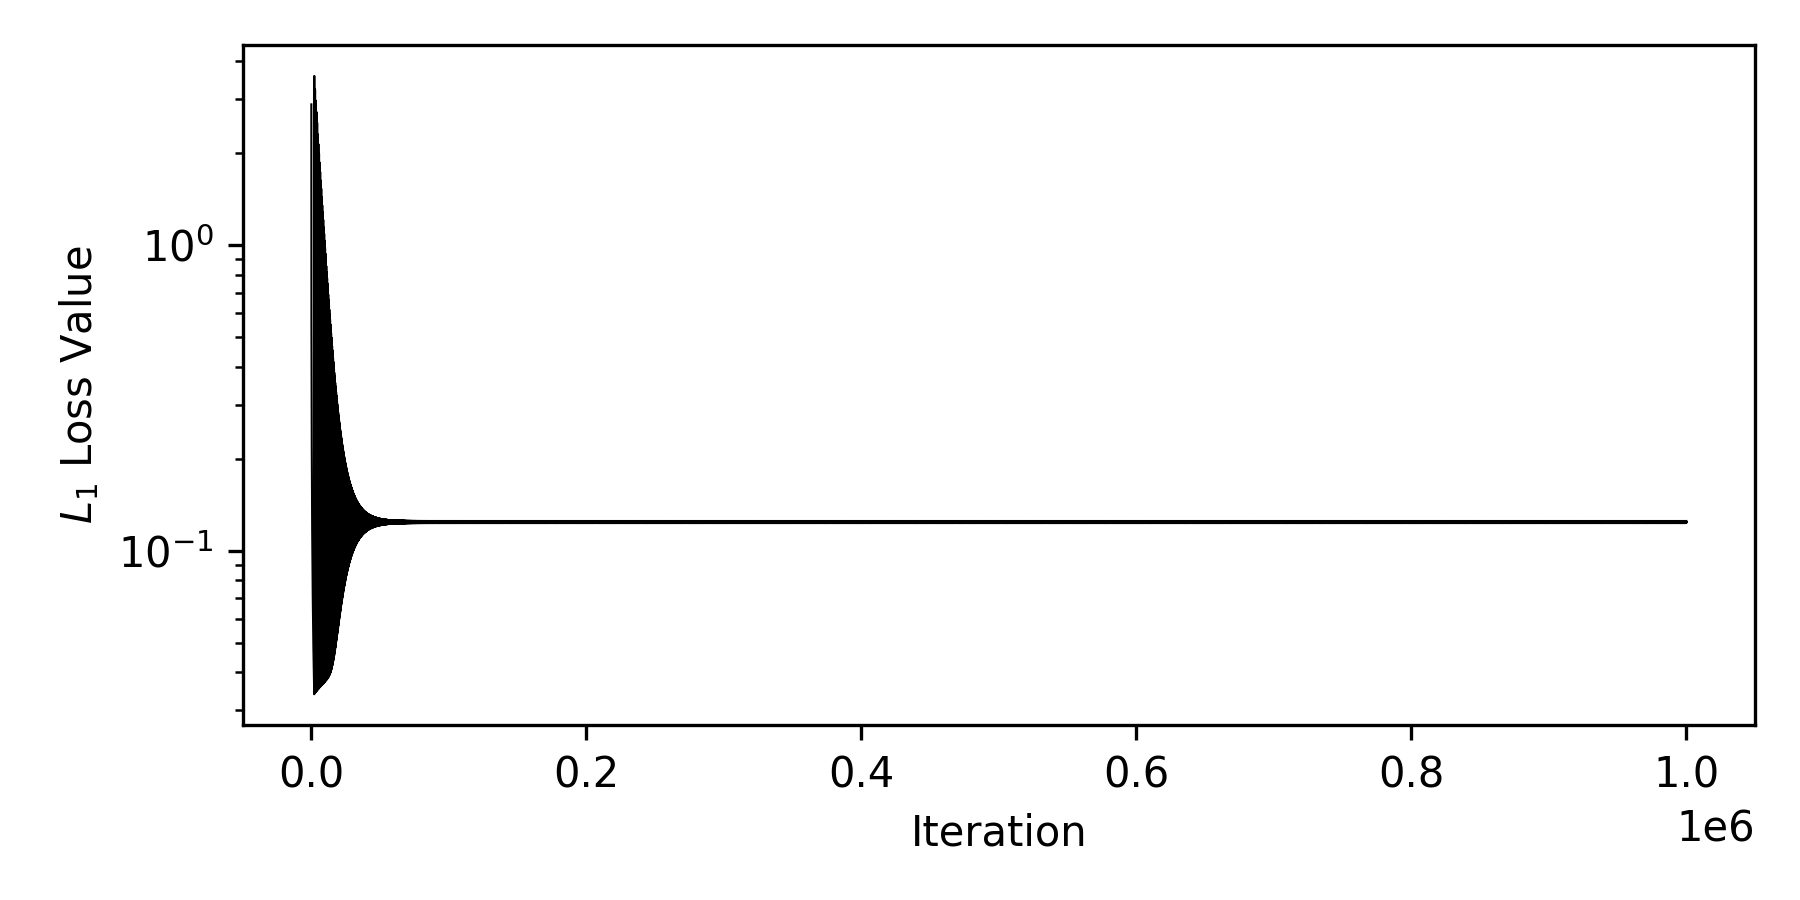
\includegraphics[width=\linewidth]{images/gd/GD_loss_plot.png}
      \caption{$\alpha =$ 1E-3}
      \label{fig:gd_1e-3}
    \end{subfigure}\hfill
    \begin{subfigure}{.5\linewidth}
      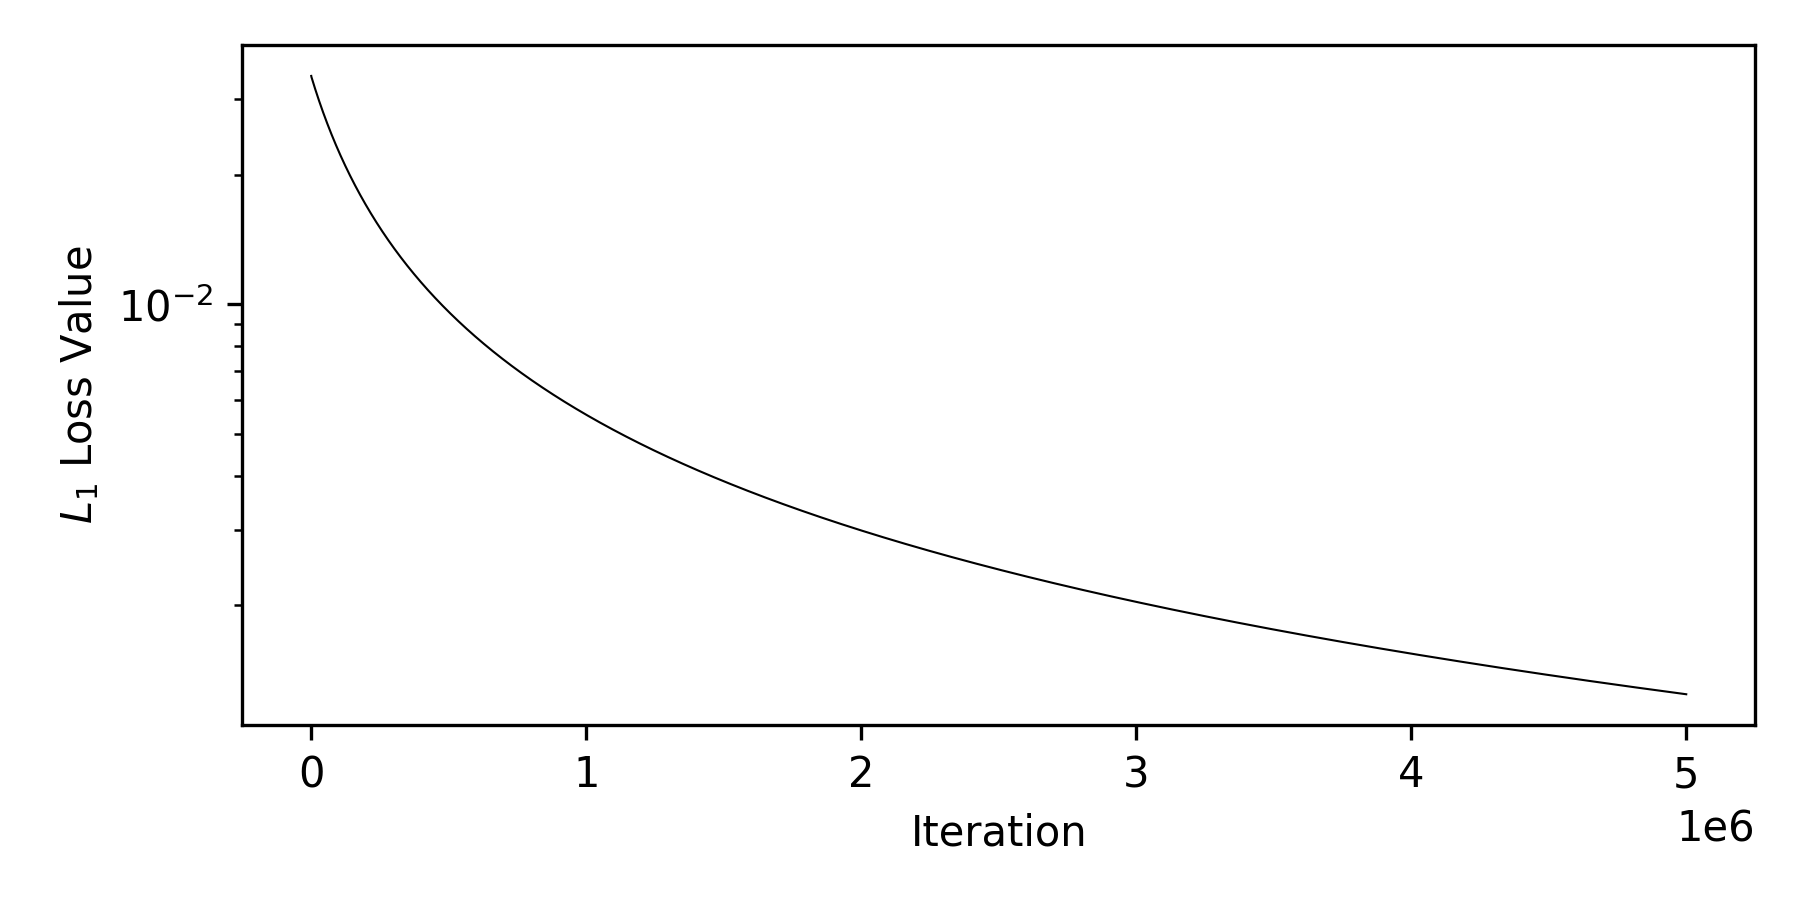
\includegraphics[width=\linewidth]{images/gd/GD_loss_plot2.png}
      \caption{$\alpha =$ 1E-5}
      \label{fig:gd_1e-5}
    \end{subfigure}
    
    \caption{Plots of the $L_1$ loss against each of the (a) 1,000,000 and (b) 5,000,000 iterations. Each contour consists of $n = 100$ points. The initial parameters used are (a) $b = 0.7$ and $y = 0.895588$ (b) $b = 0.3227341040398728$ and $y = 1.8244690757568378$. Figure (a)'s lowest score was $L_1 \approx$ 3E-2 with the initial parameters of (b). Figure (b)'s lowest score was $L_1 \approx$ 1E-3 with parameters $b = 0.14124692711511863$ and $y = 2.6503746377415633$.}
    \label{fig:GD_loss_plots}
\end{figure}

From our first attempt at the gradient descent (GD) algorithm (\autoref{fig:gd_1e-3}), we see that the $L_1$ loss converges to a higher value than the best loss of $L_1 = 0.03390312294797621 \approx$ 3E-2 with parameters $b = 0.3227341040398728$ and $y = 1.8244690757568378$. This indicates that the GD algorithm did not effectively reduce the loss suggesting that the learning rate $\alpha$ might be too high, causing the algorithm  to overshoot the optimal parameter values.

Given the suboptimal convergence observed in Figure (\ref{fig:gd_1e-3}), we ran a second set of experiments with a reduced learning rate of $\alpha = 1 \times 10^{-5}$ over 1,000,000 iterations initially. We used the parameters that achieved the best loss from our first run and we see a much better convergence rate in Figure (\ref{fig:gd_1e-5}) for the first 1,000,000 iterations. We then extend this over till we see a notable decrease in the convergence rate at around iteration $5 \times 10^{6}$. By lowering the learning rate, the GD algorithm was able to achieve a lower $L_1$ loss of $0.0012438982603344348 \approx $ 1E-3.

\begin{figure}[H]
    \begin{subfigure}{.33\linewidth}
      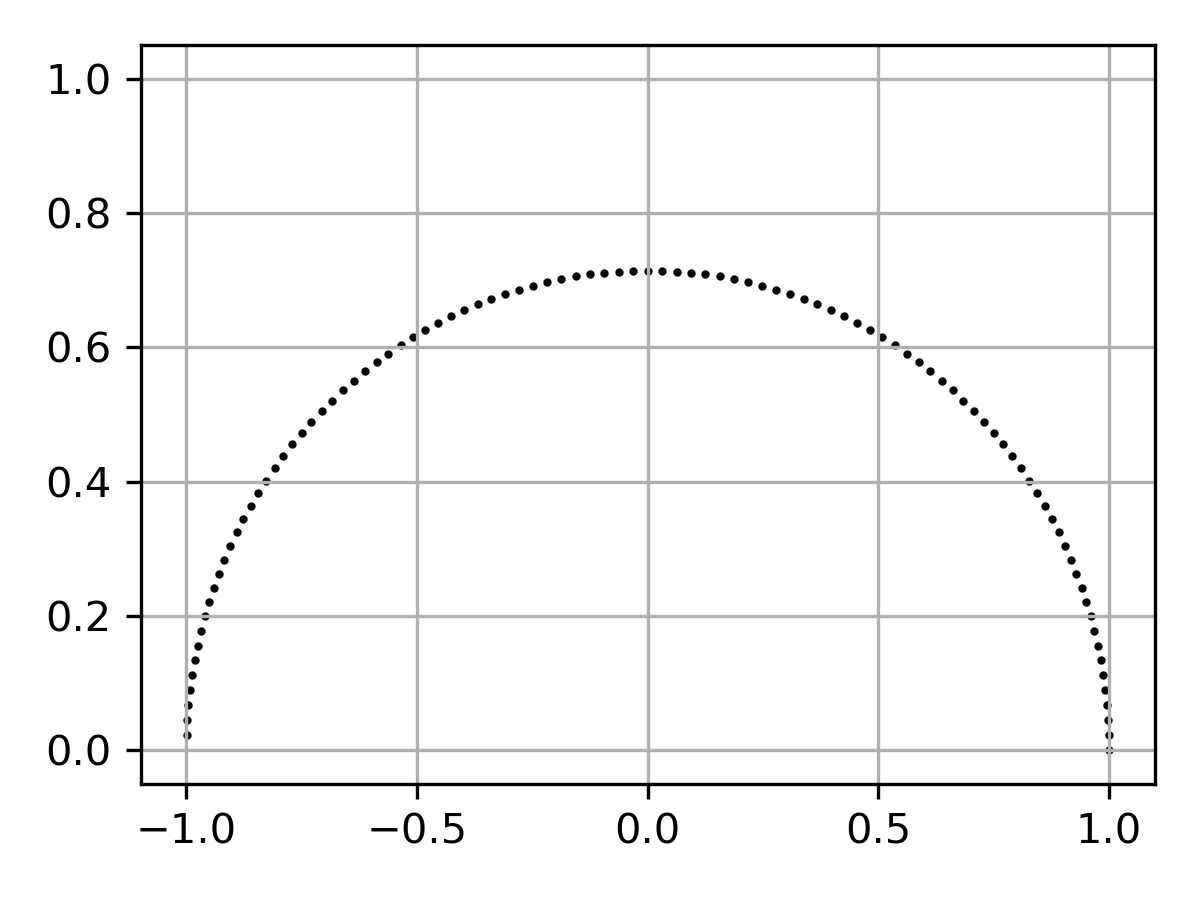
\includegraphics[width=\linewidth]{images/gd/initial_params_GD.png}
      \caption{$L_1 = 2.89186578074851$}
      \label{fig:gd_initial_params}
    \end{subfigure}\hfill
    \begin{subfigure}{.33\linewidth}
      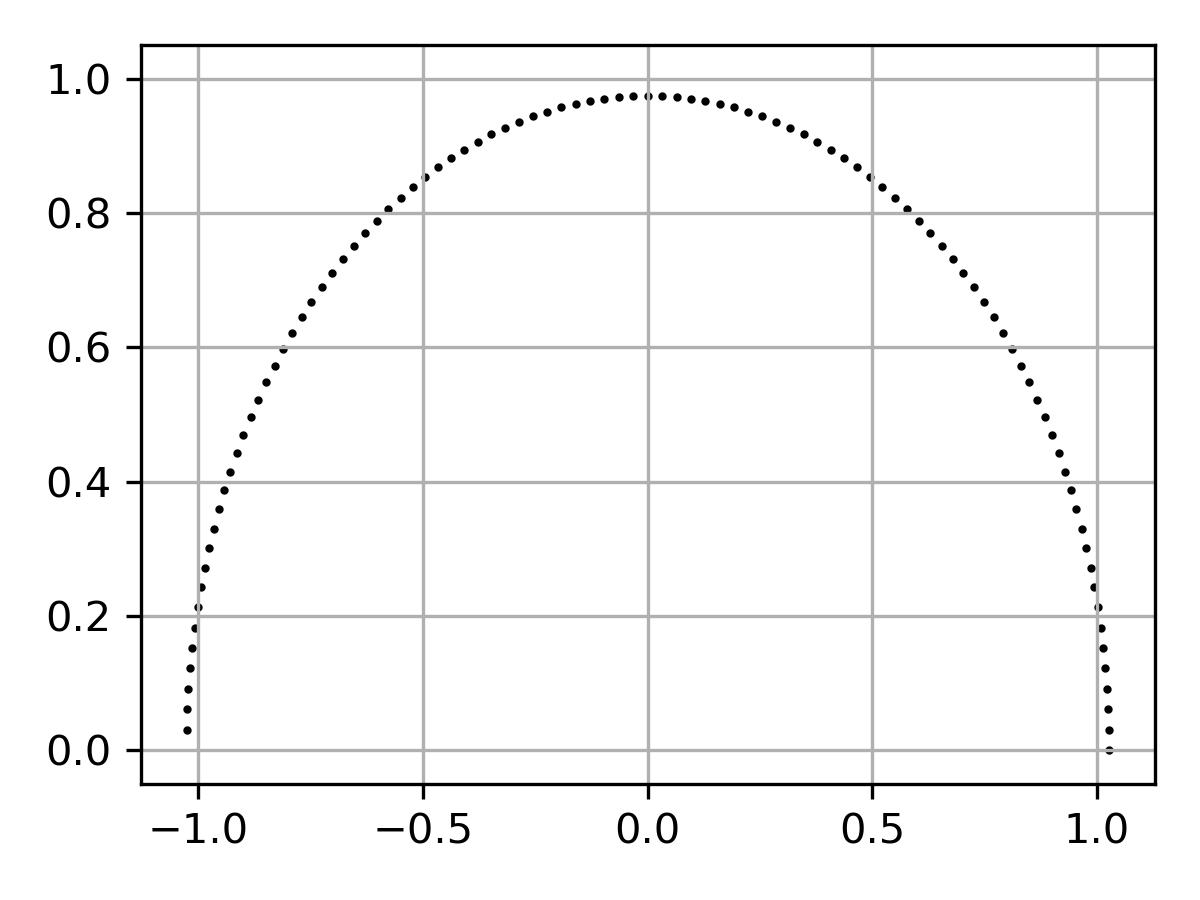
\includegraphics[width=\linewidth]{images/gd/params_after_first_GD.png}
      \caption{$L_1 = 0.03390312294797621$}
      \label{fig:gd_after_first_run}
    \end{subfigure}\hfill
    \begin{subfigure}{.33\linewidth}
      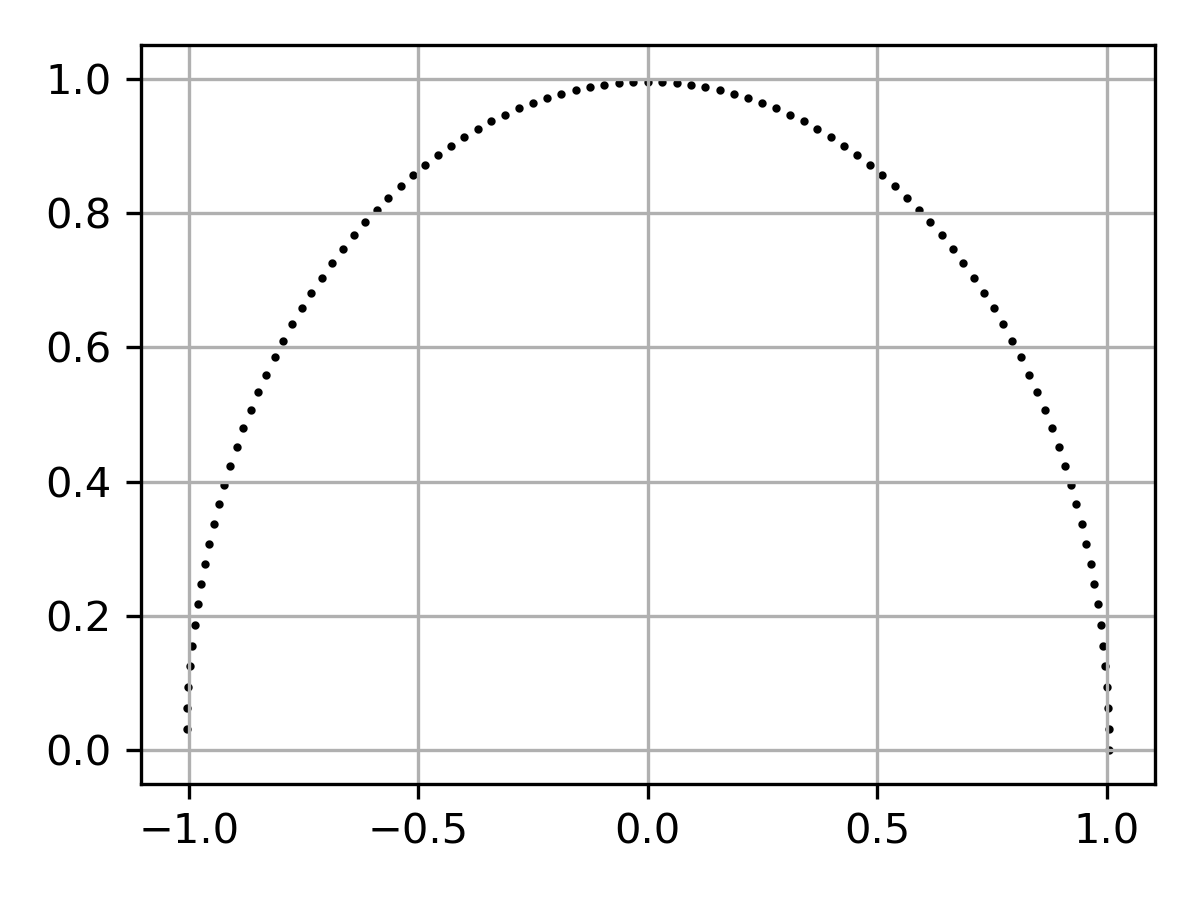
\includegraphics[width=\linewidth]{images/gd/params_after_GD.png}
      \caption{$L_1 = 0.0012438982603344348$}
      \label{fig:gd_final}
    \end{subfigure}
    
    \caption{Visualisation of the contours achieved by the gradient descent algorithm in comparison to our initial parameters with their respective $L_1$ loss values. }
    \label{fig:gd_param_visuals}
\end{figure}

Whilst we can see the gradual improvements (\autoref{fig:gd_param_visuals}), this is still very far from that of the unit circle with $L_1 \approx 7E-31$. And whilst reducing the learning rate will achieve a better loss, continuous adjustments of learning rate $\alpha$ is rather tedious practically. We thus employ ADAM optimiser in attempt to achieve a higher level of accuracy.

% ========================================
% ADAM Optimiser
% ========================================
\subsection{ADAM Optimiser}
\begin{figure}[H]
    \begin{subfigure}{.7\linewidth}
      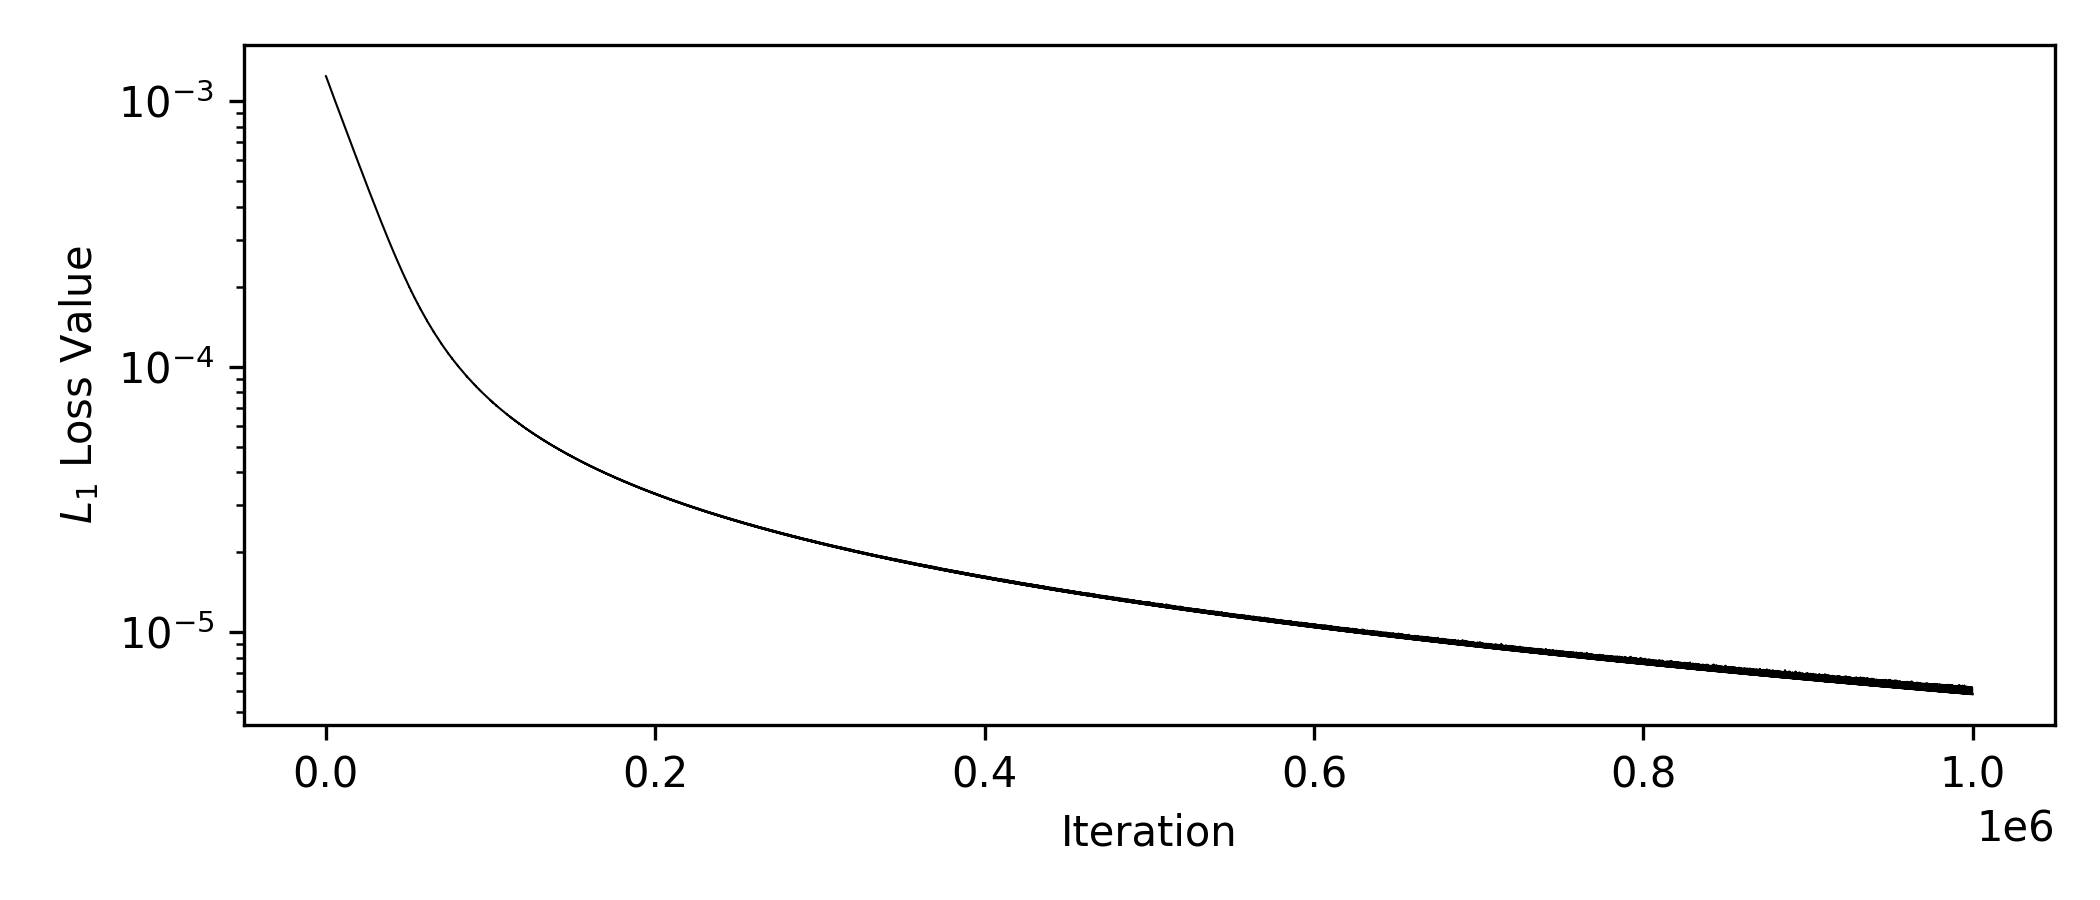
\includegraphics[width=\linewidth]{images/gd/ADAM_loss.png}
      \caption{1,000,000 iterations with $\alpha =$ 1E-5 and initial loss of $L_1 \approx$ 1.2E-3 }
    \end{subfigure}\hfill
    \begin{subfigure}{.3\linewidth}
      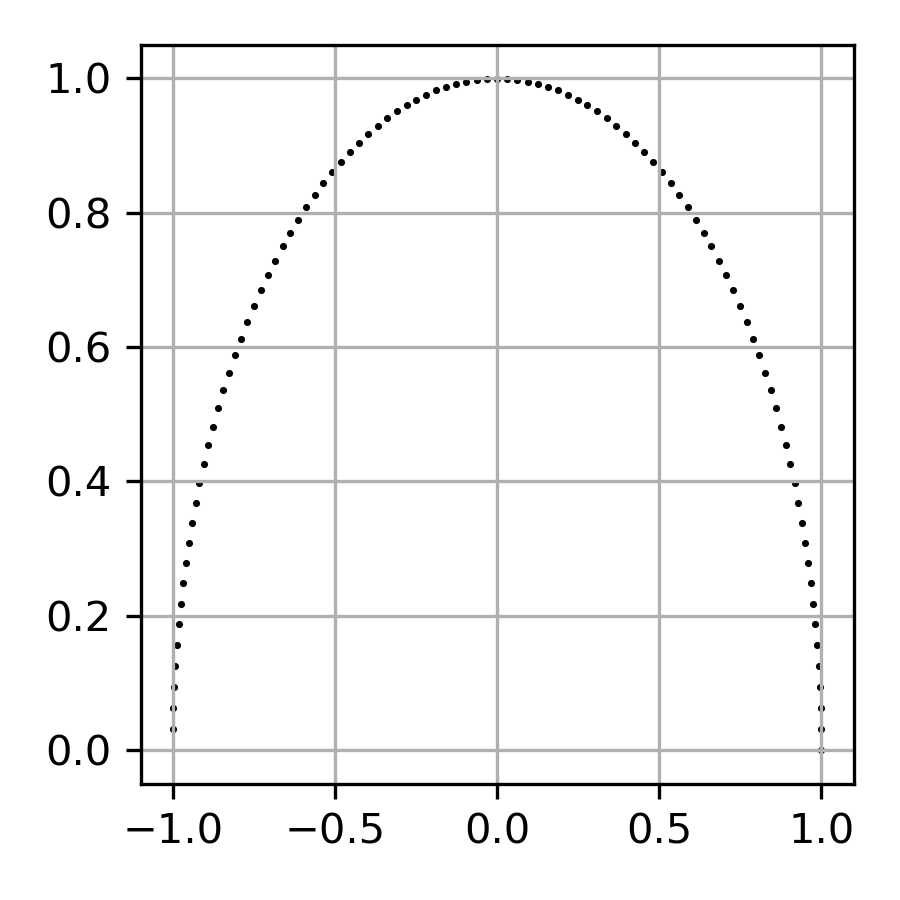
\includegraphics[width=\linewidth]{images/gd/params_after_first_ADAM.png}
      \caption{$L_1 \approx$ 5.8E-6}
      \label{fig:first_adam}
    \end{subfigure}
    
    \caption{$L_1$ loss plot over 1,000,000 iterations initialised with $n = 100$ points, $b = 0.14124692711511863 $ and $y = 2.6503746377415633$. The optimiser achieves Figure (\ref{fig:first_adam}) after its first execution constructed with parameters $b = 0.0369625708464355$ and $y = 3.9909964437511105$. }
\end{figure}

The Adaptive Moment Estimation (ADAM) optimiser provides a more sophisticated approach to parameter tuning as discussed in Section (\ref{section:ADAM}). We conducted our experiments initially with parameters set to $b = 0.14124692711511863$ and $y = 2.6503746377415633$, and the learning rate $\alpha$ was set to $1 \times 10^{5}$. At first glance, we see a much a better convergence and $L_1$ loss in Figure (\ref{fig:first_adam}), plotted over 1,000,000 iterations, compared to Figure (\ref{fig:gd_1e-5}), plotted over 5,000,000 iterations. We thus reiterate the experiment but change the initial parameters in hopes of achieving a better $L_1$ score. 

Here, we document the results of various runs with re-feeding the parameters back-to-back for each run. The table below lists the best $L_1$ losses during different stages of these runs.

\begin{table}[ht]
\centering
\begin{tabular}{|l|l|l|}
\hline
b & y & $L_1$ Loss \\
\hline
0.023601865718395856 & 4.4395753229571016 & 9.888987368769754E-07 \\
0.012128186643020126 & 5.105370236695753 & 6.761351664008986E-08 \\
0.006856851878987493 & 5.675654087958846 & 6.90825126014524E-09 \\
0.0016260199411660154 & 7.114767183400269 & 2.1845205202267918E-11 \\
0.0010793477830991617 & 7.5245455065711715 & 4.241412093544462E-12 \\
1.2712609608154088E-05 & 11.966063364769047 & 9.33039337162676E-15 \\
1.2786721545826545E-05 & 11.960250483055397 & 4.955043180518183E-16 \\
6.515415674882209E-05 & 10.331901633745023 & 8.120200210832519E-17 \\
1.4883598328756484E-05 & 11.80839791524078 & 4.682445773102879E-19 \\
1.48835270677098E-05 & 11.808402703087143 & 1.5334589506224306E-19 \\
\hline
\end{tabular}
\caption{Best $L_1$ loss, with corresponding parameters $b$ and $y$,  achieved during several stages of the runs using ADAM optimiser with varying initial learning rates of 1E-3 $\leq \alpha \leq$ 1E-7.}
\end{table}

After multiple runs and tinkering of the hyper-parameters, we achieve a loss of $L_1 \approx$ 1.5E-19 with parameters $b = 1.48835270677098$E-05 and $y = 11.808402703087143$. Whilst we were unable to find better parameters given the time constraints of this project, we deem this sufficient enough given the similarity to that of the unit circle, with a loss of $L_1 \approx$ 7E-31. This is visually shown in the following figure:
\begin{figure}[H]
    \begin{subfigure}{.5\linewidth}
      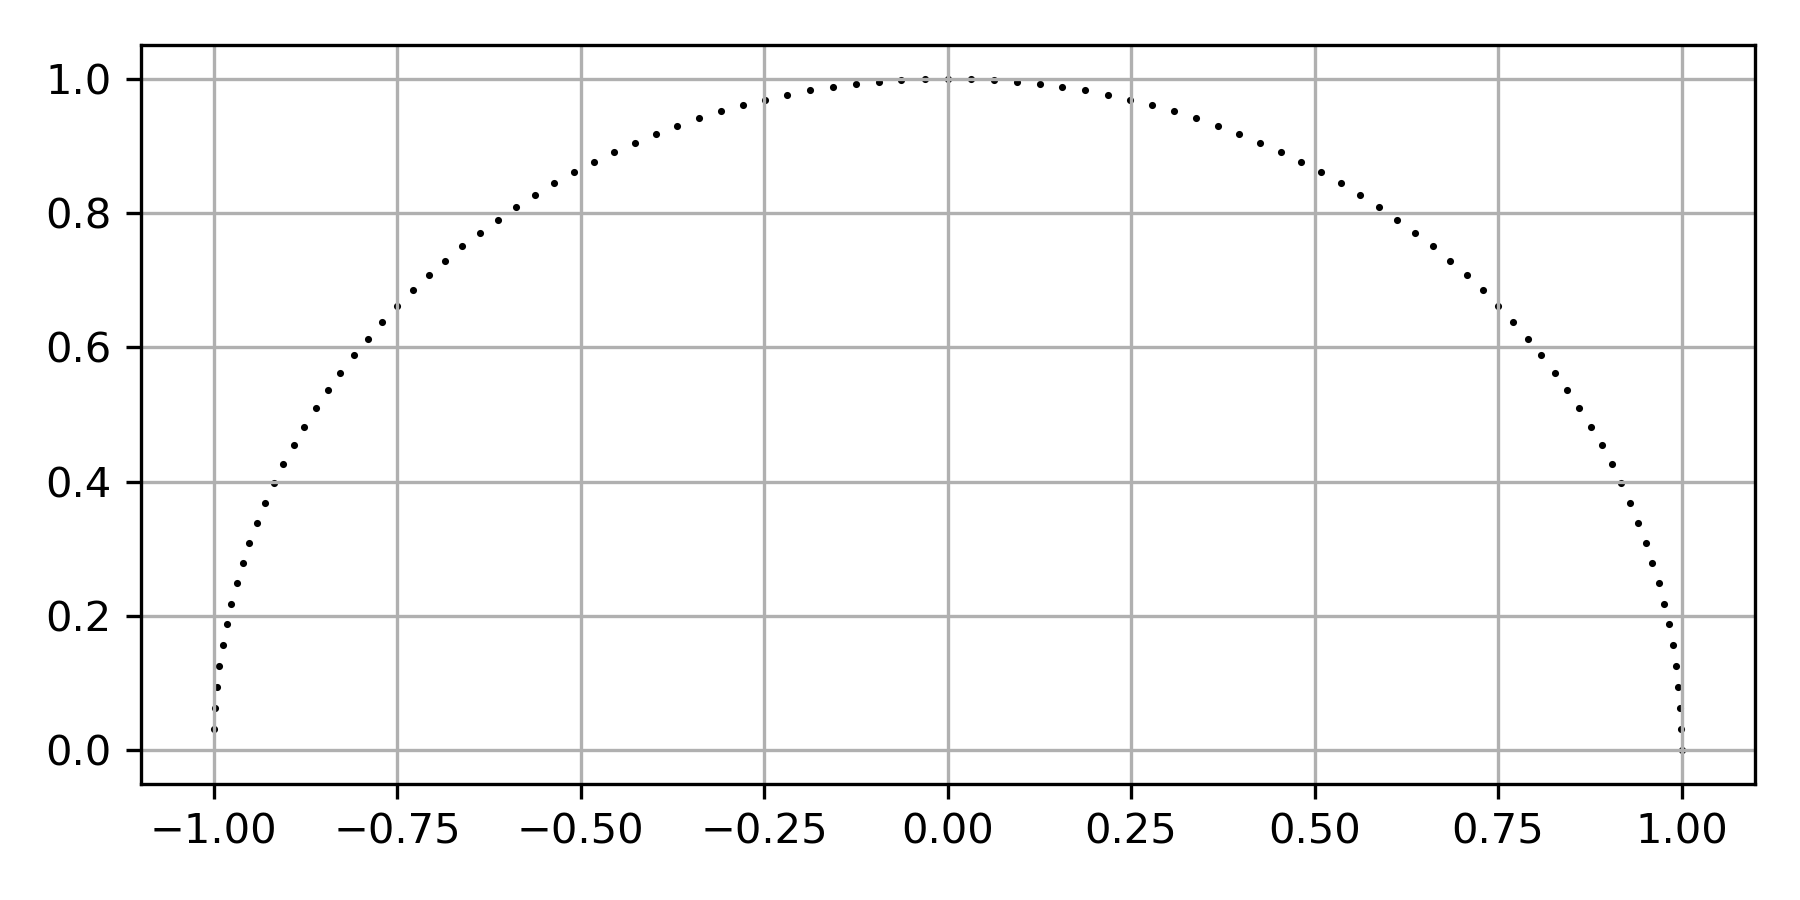
\includegraphics[width=\linewidth]{images/gd/unit_circle.png}
      \caption{Circle Contour: $z = re^{i\theta}$}
      \label{fig:circle_contour}
    \end{subfigure}\hfill
    \begin{subfigure}{.5\linewidth}
      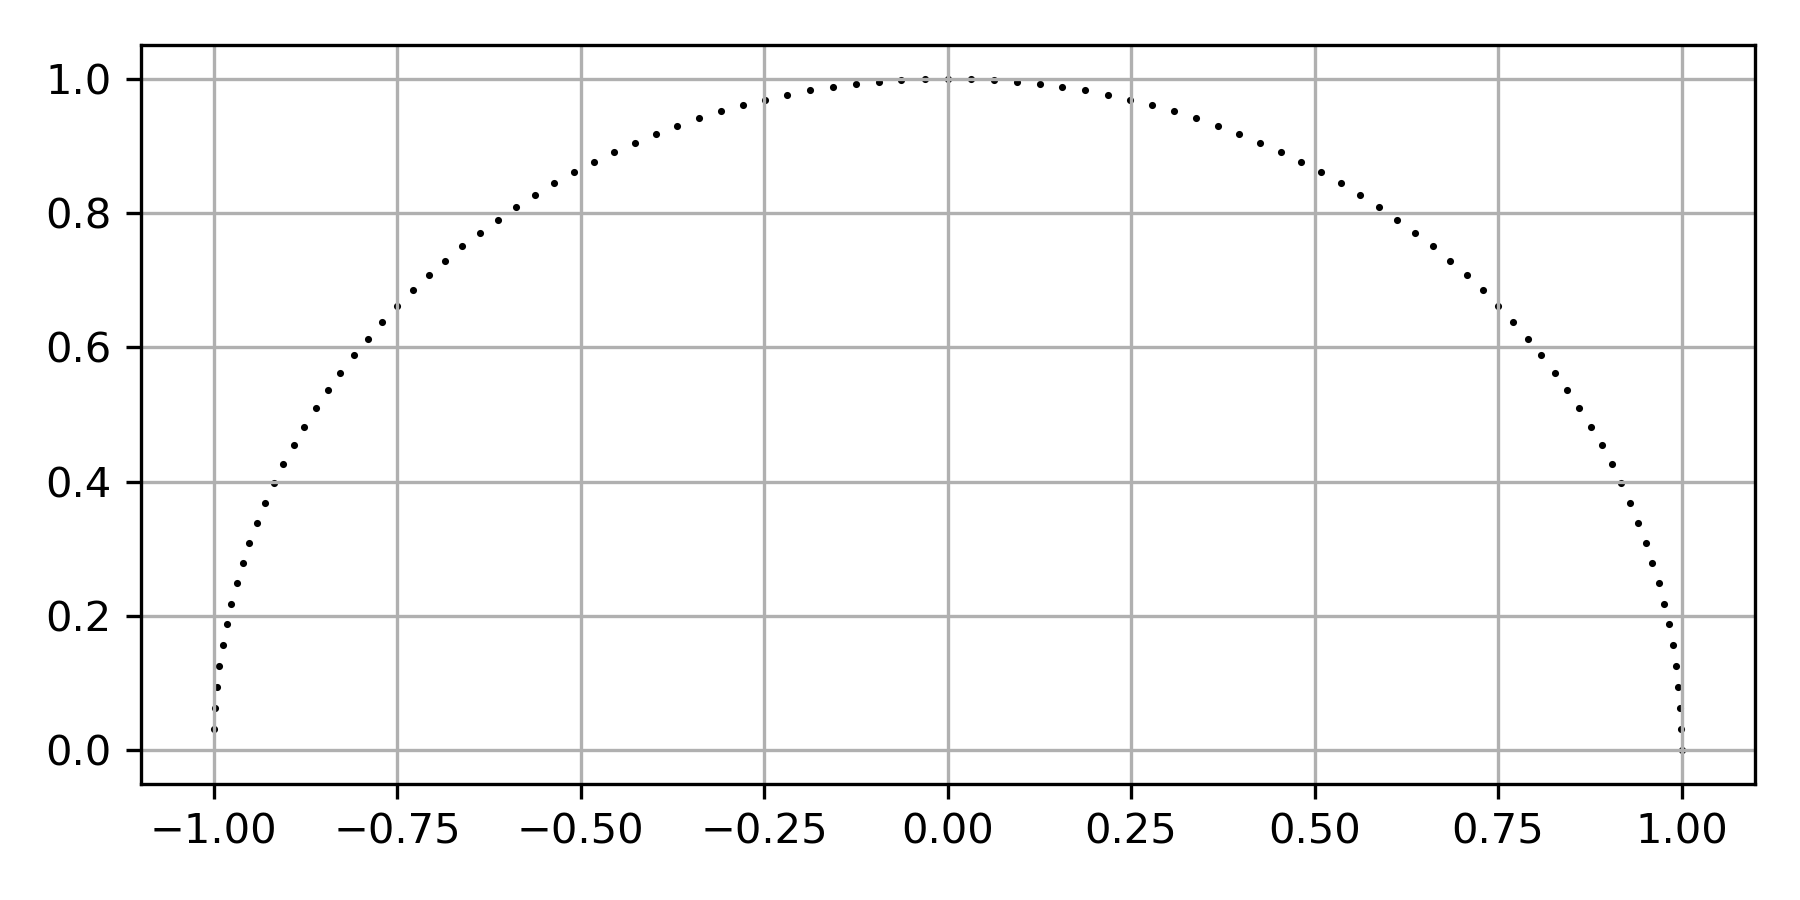
\includegraphics[width=\linewidth]{images/gd/best_params.png}
      \caption{Sinh Deformation: $\sigma + ib\sinh(\omega + y)$}
      \label{fig:perfect_sinh}
    \end{subfigure}
    
    \caption{Visual representation for $n = 100$ points of the (a) circle contour with $r = 1$ and $0 \leq \theta < \pi$, and (b) sinh deformation with $\sigma = 0.0$, $b = 1.48835270677098$E-05, $y = 11.808402703087143$ and $-\frac{\pi}{2} \leq \omega < \frac{\pi}{2}$.}
\end{figure}

As discussed in Section (\ref{section:point_distance}), we check to see the average distance between each point of both the circular contour and the sinh deformation. In an idealistic setting, we expect the difference between each point to be $\frac{\pi}{99} \approx 0.03173325912716963$ as shown in Example (\ref{example:point_diff}). Figure (\ref{fig:circle_contour}) has an average distance of 0.03172875474309711  whilst Figure (\ref{fig:perfect_sinh}) has an average distance of 0.031728754743097394.

% ========================================
% Numerical Benchmarking
% ========================================
\section{Numerical Benchmarking}

% ========================================
% Abate and Whitt 1992
% ========================================
\subsection{Abate and Whitt 1992}

\begin{figure}[H]
    \begin{subfigure}{.5\linewidth}
      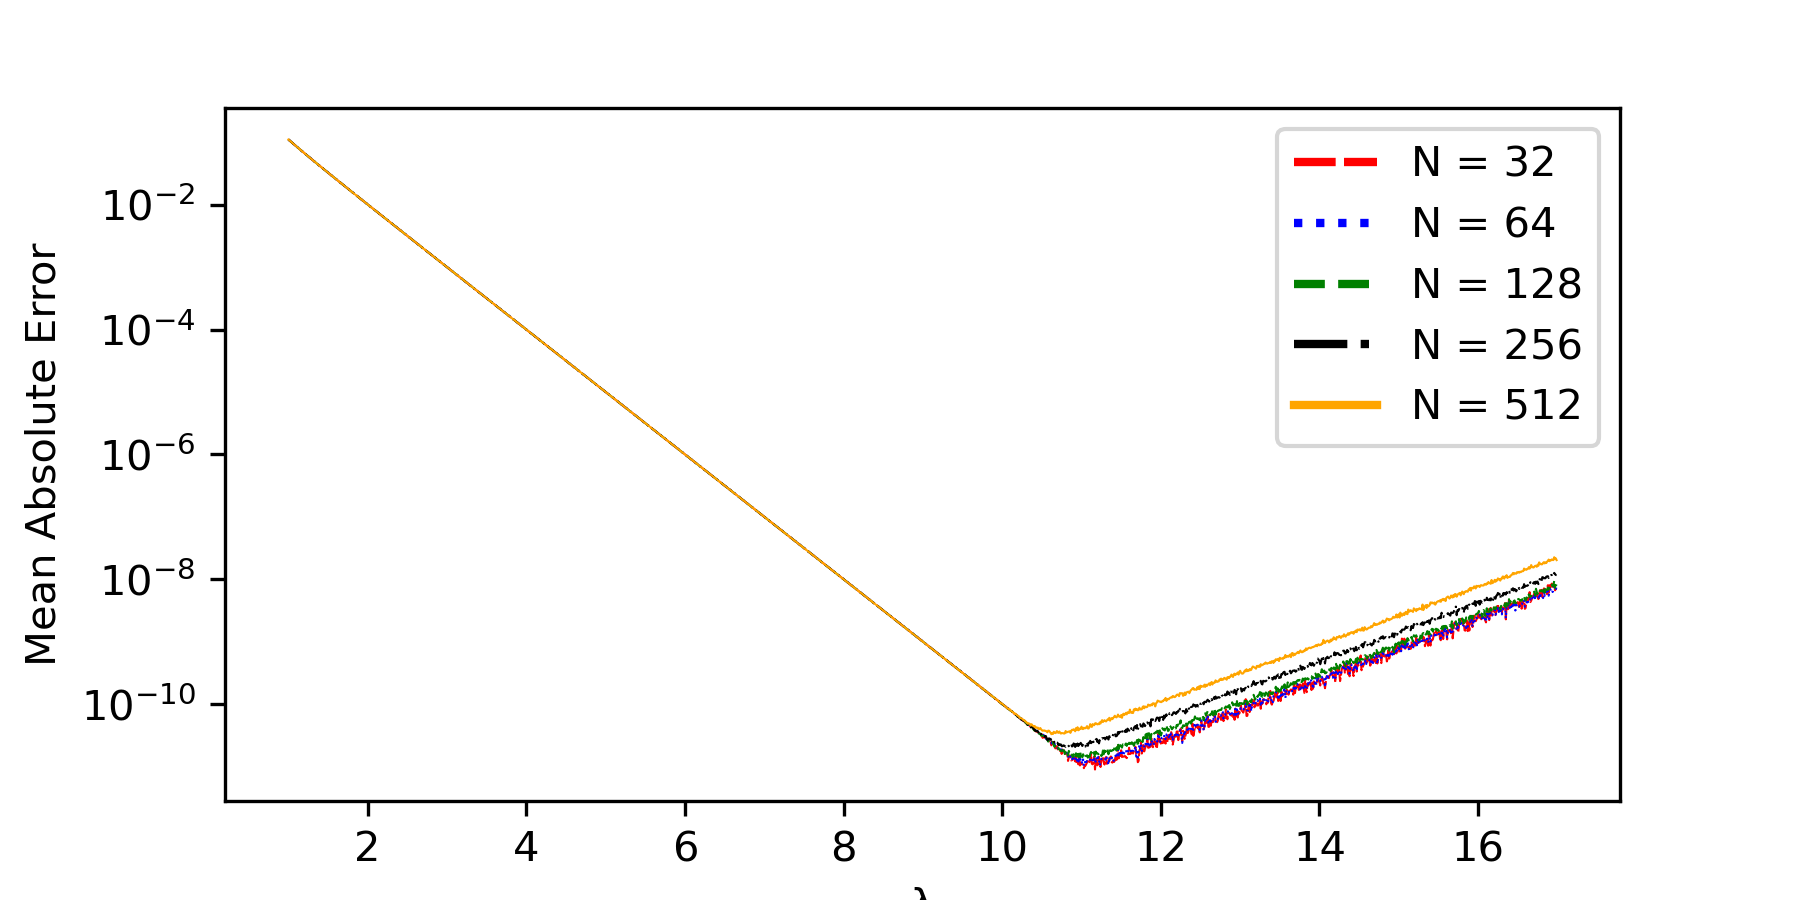
\includegraphics[width=\linewidth]{images/abate_whitt/heaviside.png}
      \caption{Heaviside Step ($1 \leq \lambda \leq 17$)}
    \end{subfigure}\hfill
    \begin{subfigure}{.5\linewidth}
      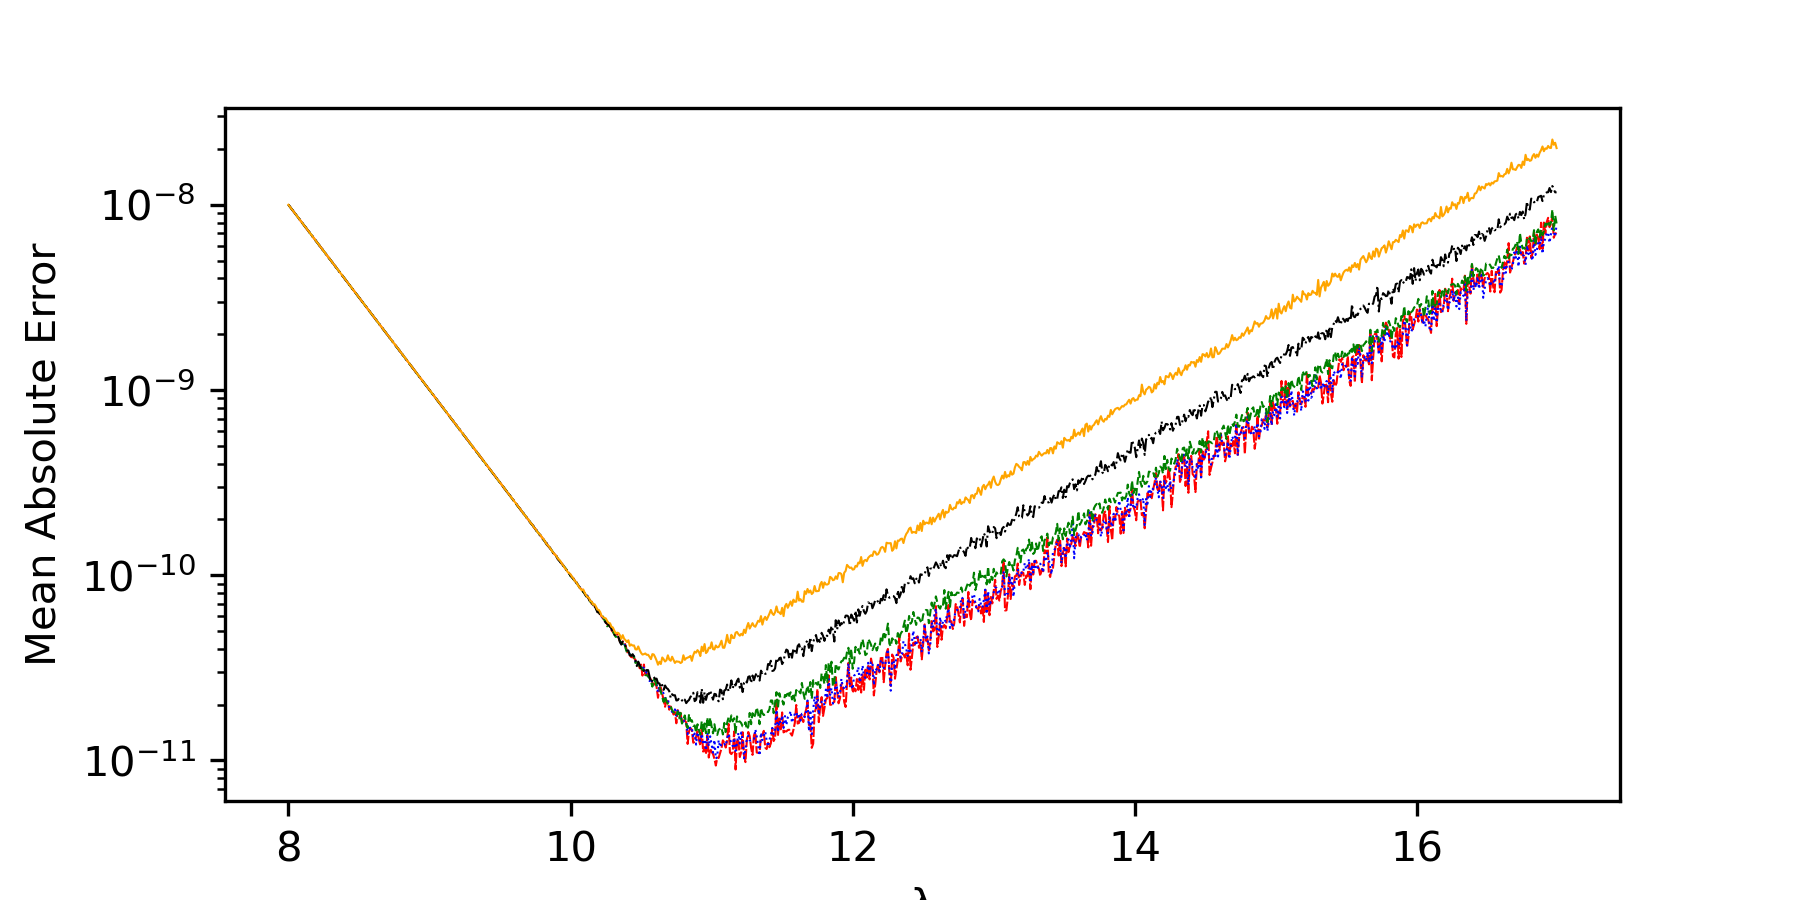
\includegraphics[width=\linewidth]{images/abate_whitt/heaviside_zoomed.png}
      \caption{Heaviside Step ($8 \leq \lambda \leq 17$)}
    \end{subfigure}
    
    \medskip
    
    \begin{subfigure}{.5\linewidth}
      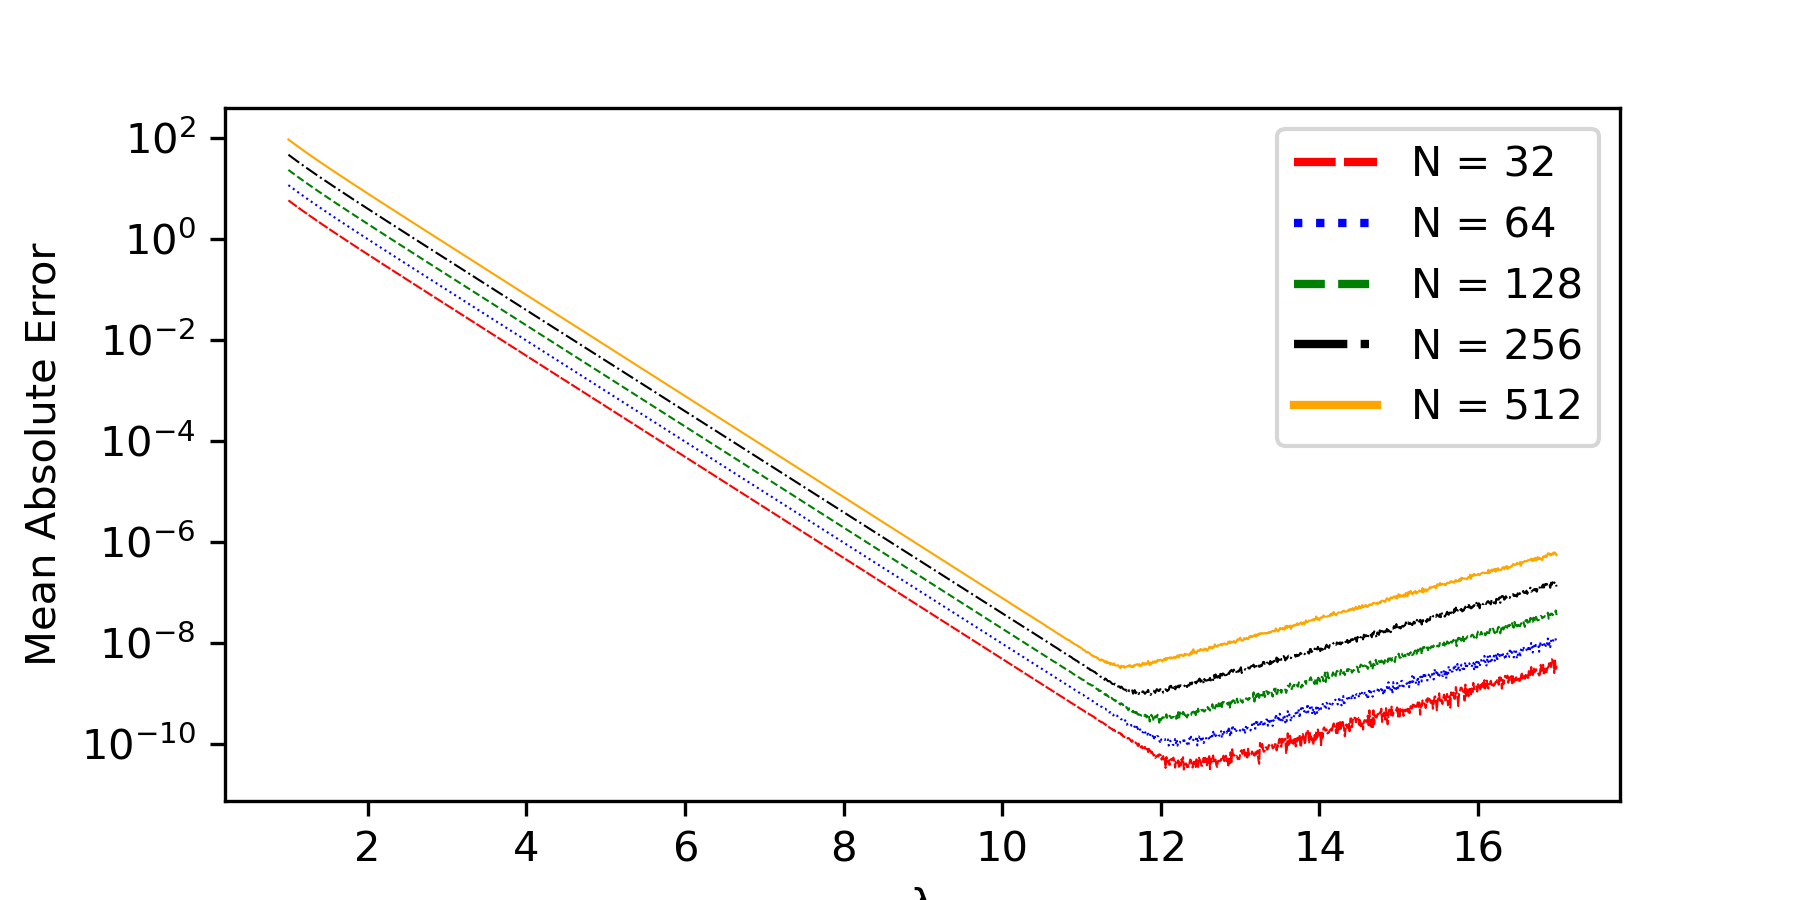
\includegraphics[width=\linewidth]{images/abate_whitt/polynomial.png}
      \caption{Polynomial ($1 \leq \lambda \leq 17)$}
    \end{subfigure}\hfill
    \begin{subfigure}{.5\linewidth}
      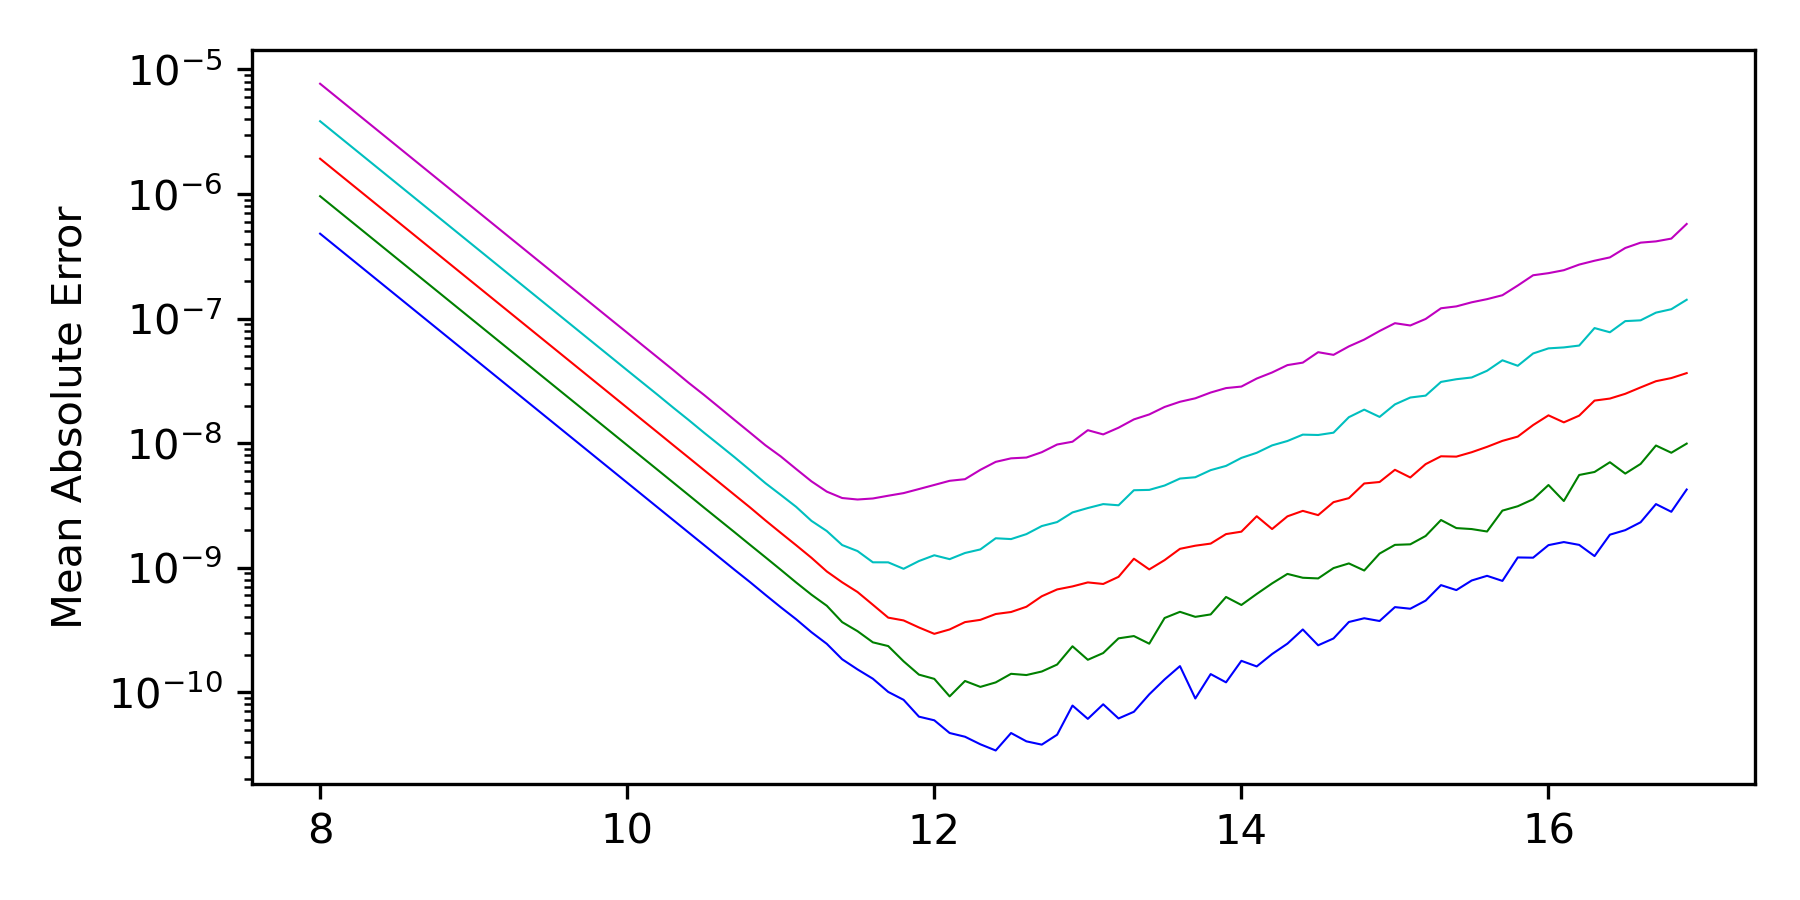
\includegraphics[width=\linewidth]{images/abate_whitt/polynomial_zoomed.png}
      \caption{Polynomial ($8 \leq \lambda \leq 17$)}
    \end{subfigure}
    
    \medskip
    
    \begin{subfigure}{.5\linewidth}
      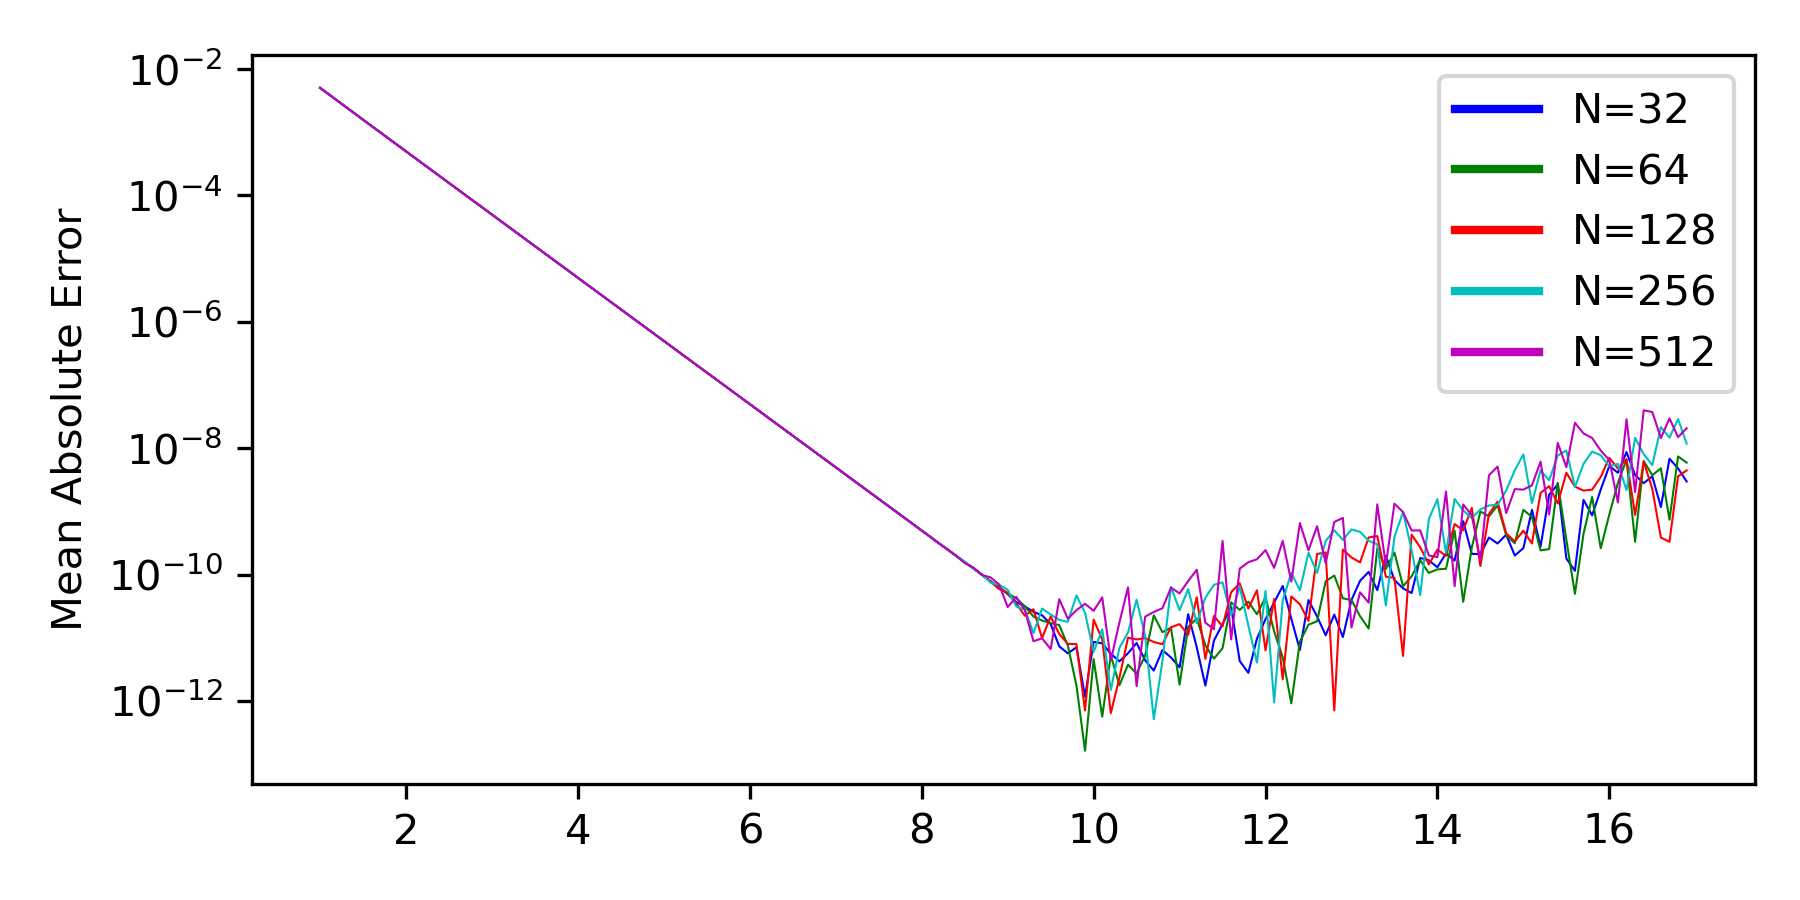
\includegraphics[width=\linewidth]{images/abate_whitt/decaying_exp.png}
      \caption{Decaying Exponential ($1 \leq \lambda \leq 17)$}
    \end{subfigure}\hfill
    \begin{subfigure}{.5\linewidth}
      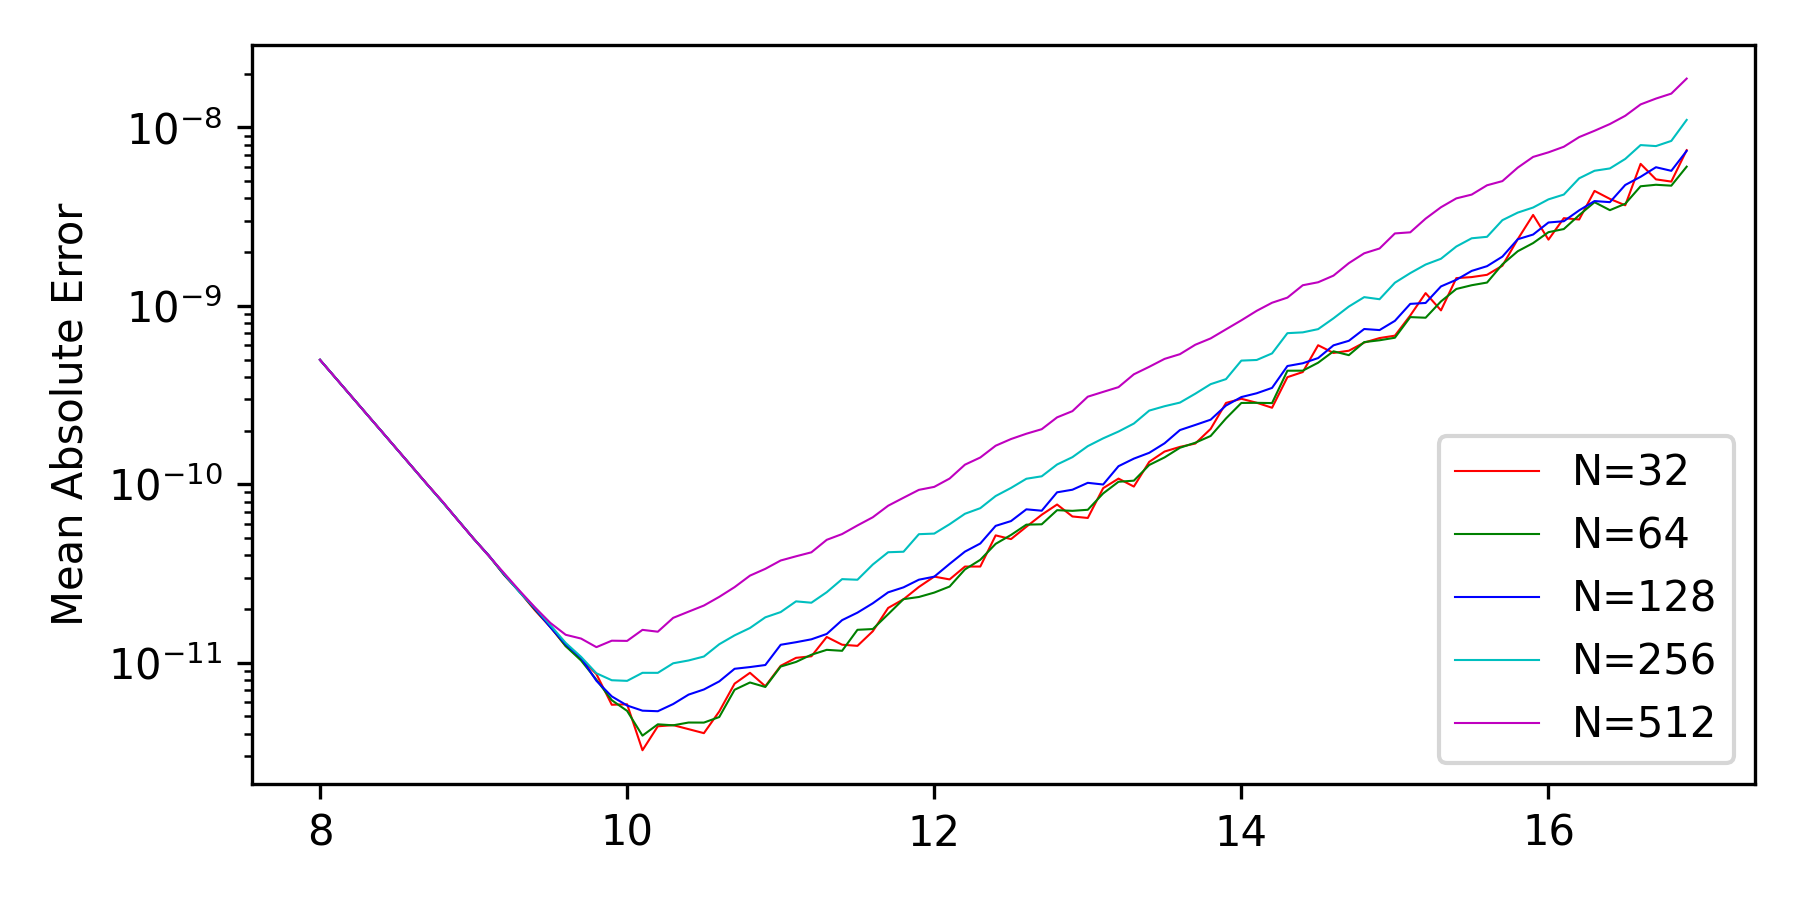
\includegraphics[width=\linewidth]{images/abate_whitt/decaying_exp_zoomed.png}
      \caption{Decaying Exponential ($8 \leq \lambda \leq 17$)}
    \end{subfigure}
    
    \todo[inline]{Add Decay Exp \& Sinusoidal}
    \caption{Mean absolute error (MAE) of the Abate-Whitt method for different values of $\lambda$ when applied to the transform pairs: (a, b) Heaviside Step, (c, d) Polynomial and (e, f) Decaying Exponential with $a = 0.1$ and $t = 10$. The MAE is plotted on a logarithmic scale against $\lambda$ values, where $\triangle \lambda = 0.1$. The different lines represent the MAE for values of N: 32, 64, 128, 256, 512.}
    \label{fig:MAE_Abate_Whitt}
\end{figure}

\begin{figure}[H]
    \begin{subfigure}{1\linewidth}
      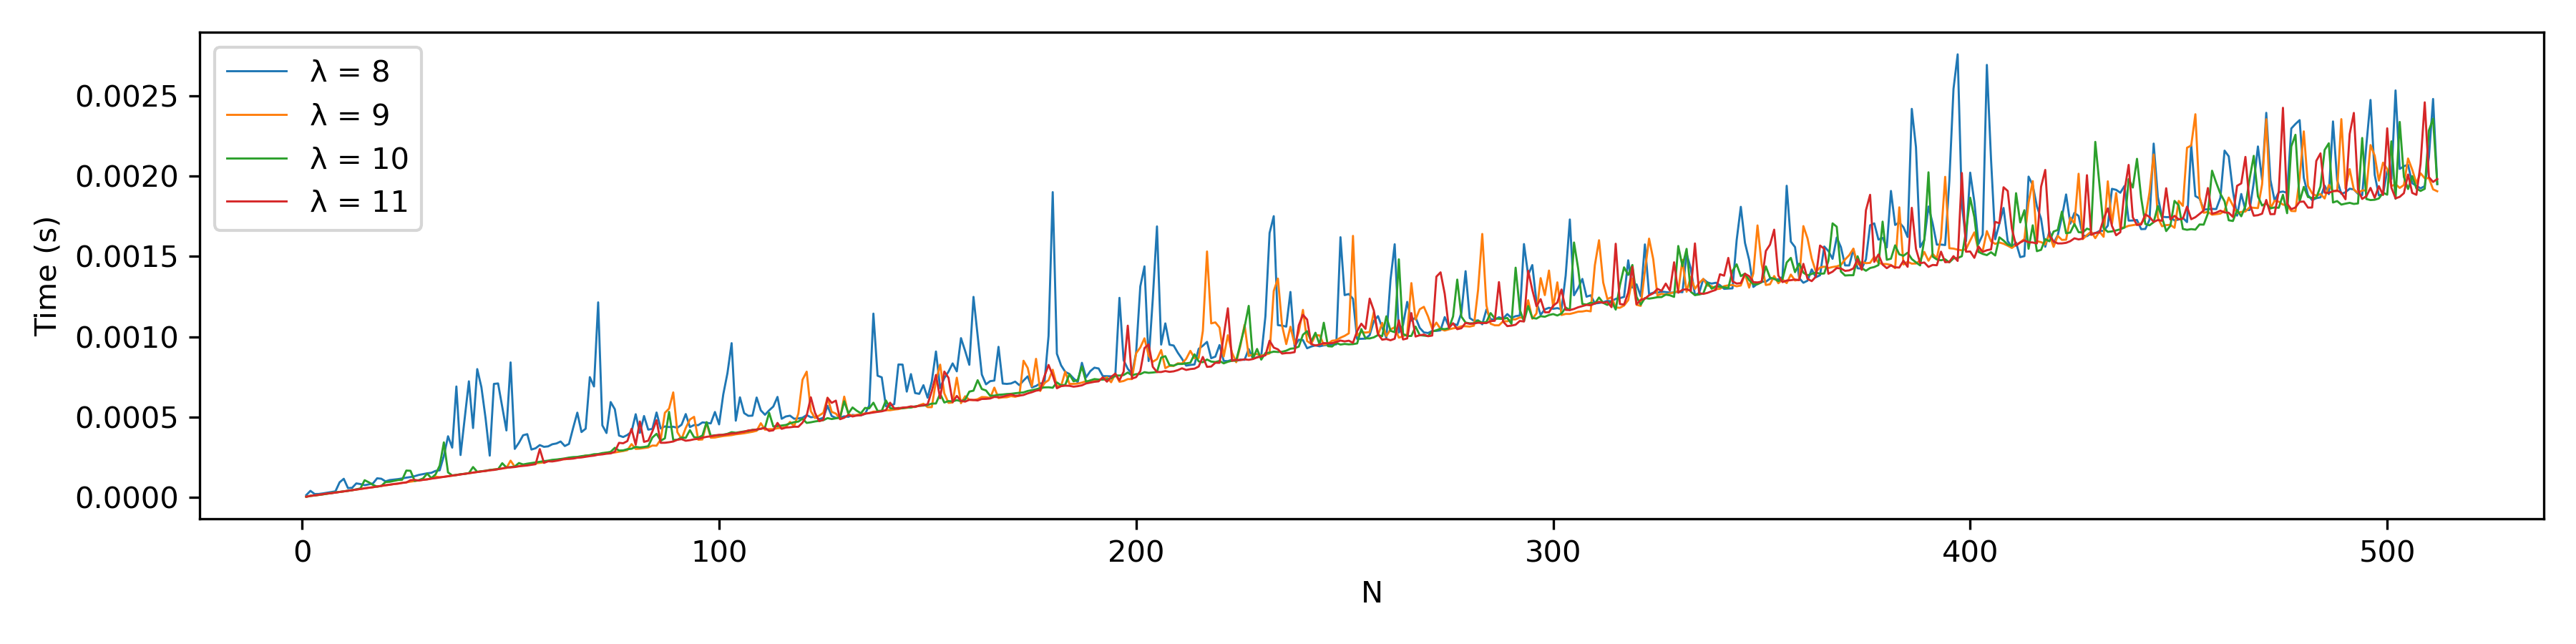
\includegraphics[width=\linewidth]{images/abate_whitt/heaviside_speed.png}
      \caption{Heaviside Step}
    \end{subfigure}
    
    \medskip
    
    \begin{subfigure}{1\linewidth}
      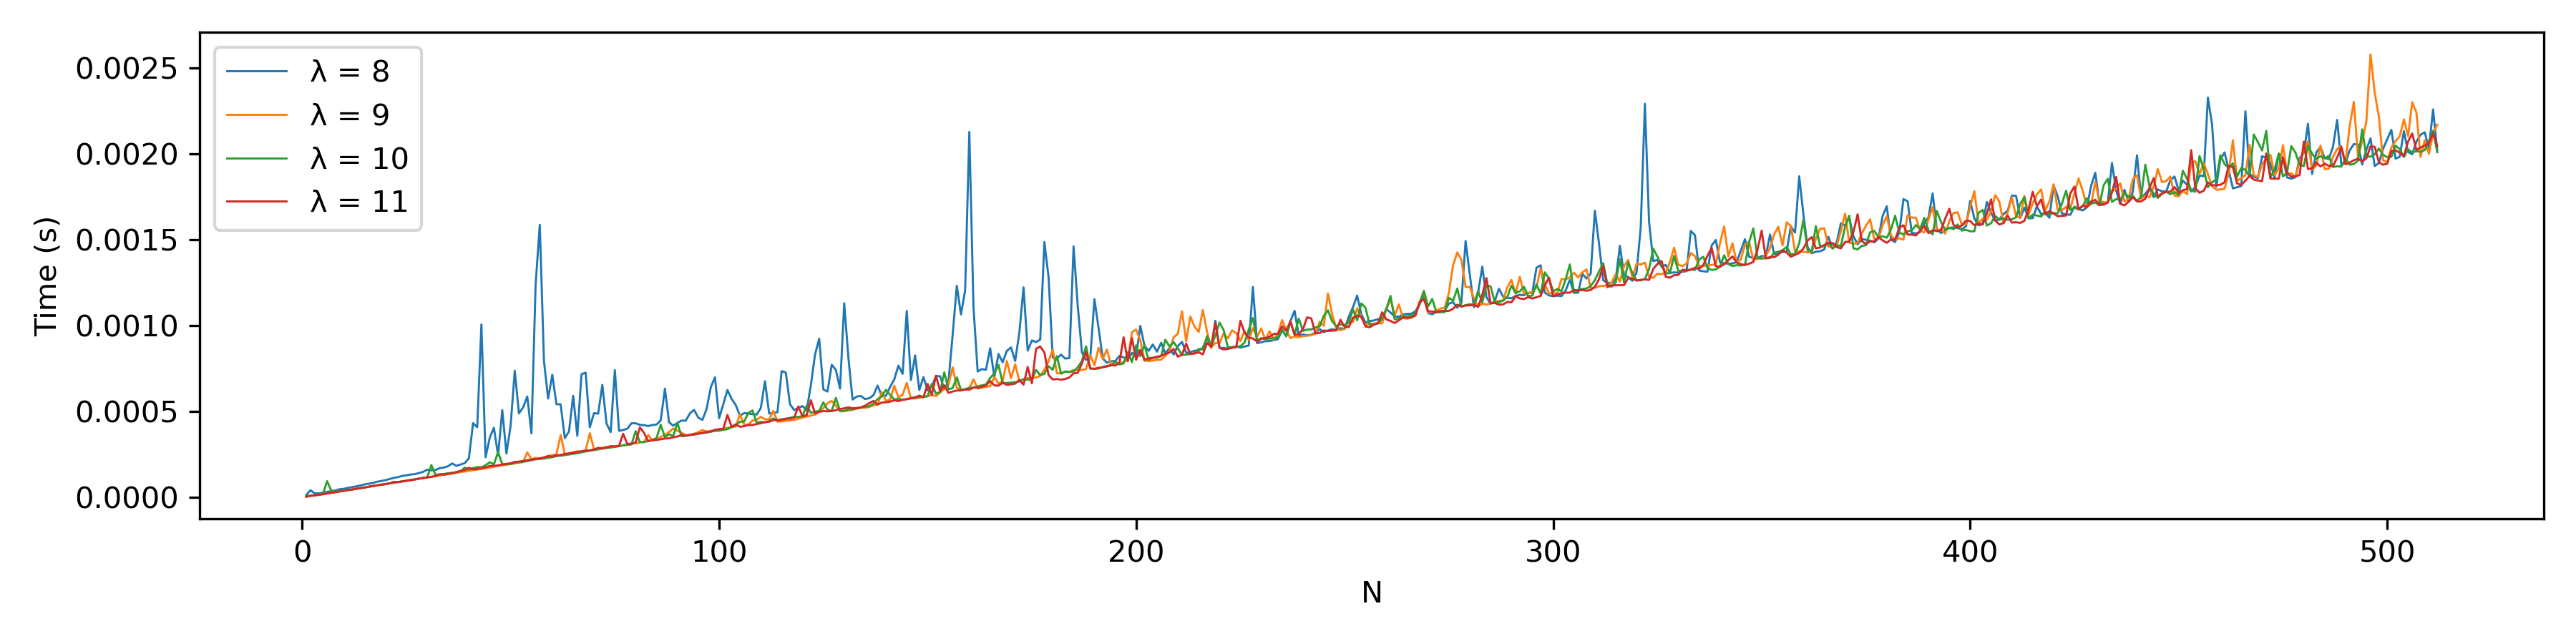
\includegraphics[width=\linewidth]{images/abate_whitt/polynomial_speed.png}
      \caption{Polynomial}
    \end{subfigure}
    
    \medskip
    
    \begin{subfigure}{1\linewidth}
      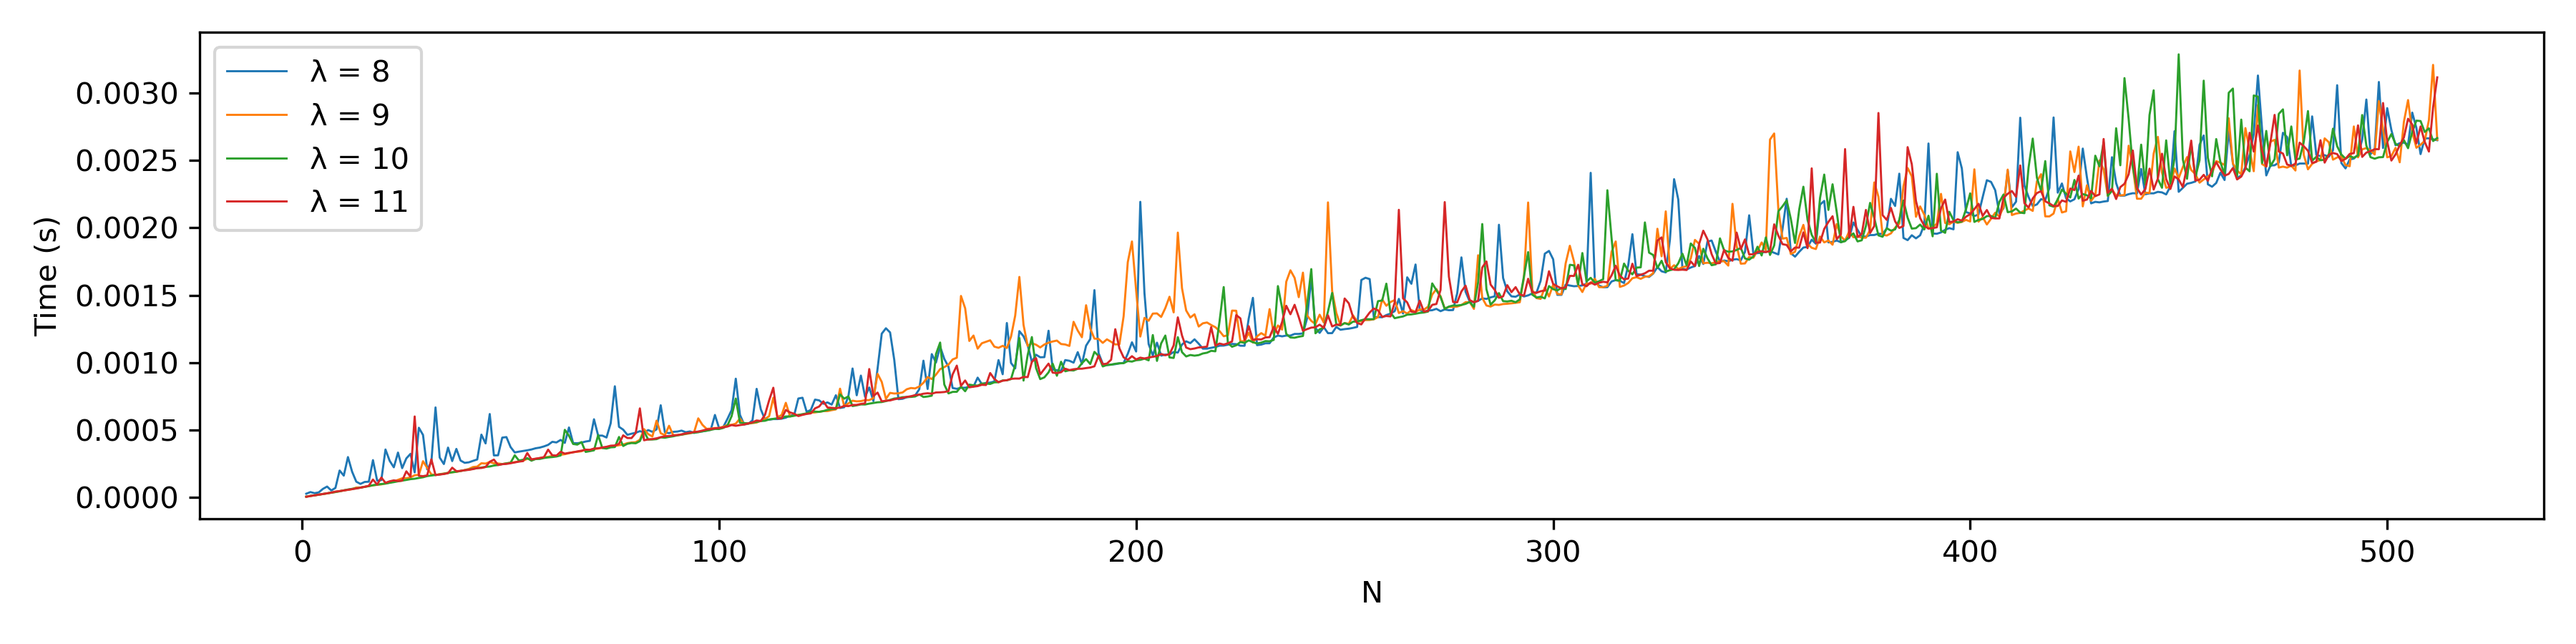
\includegraphics[width=\linewidth]{images/abate_whitt/decay_exp_speed.png}
      \caption{Decaying Exponential}
    \end{subfigure}
    
    \todo[inline]{Compute on PC averaging times over 20 runs + results for Sinusoidal}
    \caption{Timings, in seconds, of the Abate-Whitt method for different values of $N$ when applied to the (a) Heaviside Step, (b) Polynomial, and (c) Decaying Exponential transform pairs. The different lines represent the chosen $\lambda$ for each run.}
    \label{fig:timings_abate_whitt}
\end{figure}

% ========================================
% Cavers 1972
% ========================================
\subsection{Cavers 1972}


% ========================================
% Comparative Analysis
% ========================================
\subsection{Comparative Analysis}
\begin{itemize}
	\item Select few N's and hyper-parameter choices
	\item Abate Whitt vs Cavers: Transform Pair, Method, Hyper-Parameters, Actual, Estimated, Accuracy, Time	
\end{itemize}


% ========================================
% Conclusion
% ========================================
\chapter{Conclusion}

% ========================================
% Summary
% ========================================
\section{Summary}

% ========================================
% Future Work
% ========================================
\section{Future Work}

\subsection{Series Acceleration}

% ========================================
% Parameter Selection
% ========================================
\subsection{Parameter Selection}
During the course of the project, there was no set method for selecting the parameters for Equation \ref{equation:conformal_mapping}, hence, our effort of employing numerous techniques in an attempt to find the optimal parameters. However, as of recently at the time of writing, \citet{boyarchenko2024efficient} have released a paper detailing parameter selection for the conformal mapping (\ref{equation:conformal_mapping}).

% ========================================
% References 
% ========================================
\addcontentsline{toc}{chapter}{References}
\bibliography{references}
\bibliographystyle{apalike}

% ========================================
% Appendix
% ========================================
\begin{appendices}

%\chapter{Initial Project Plan}
%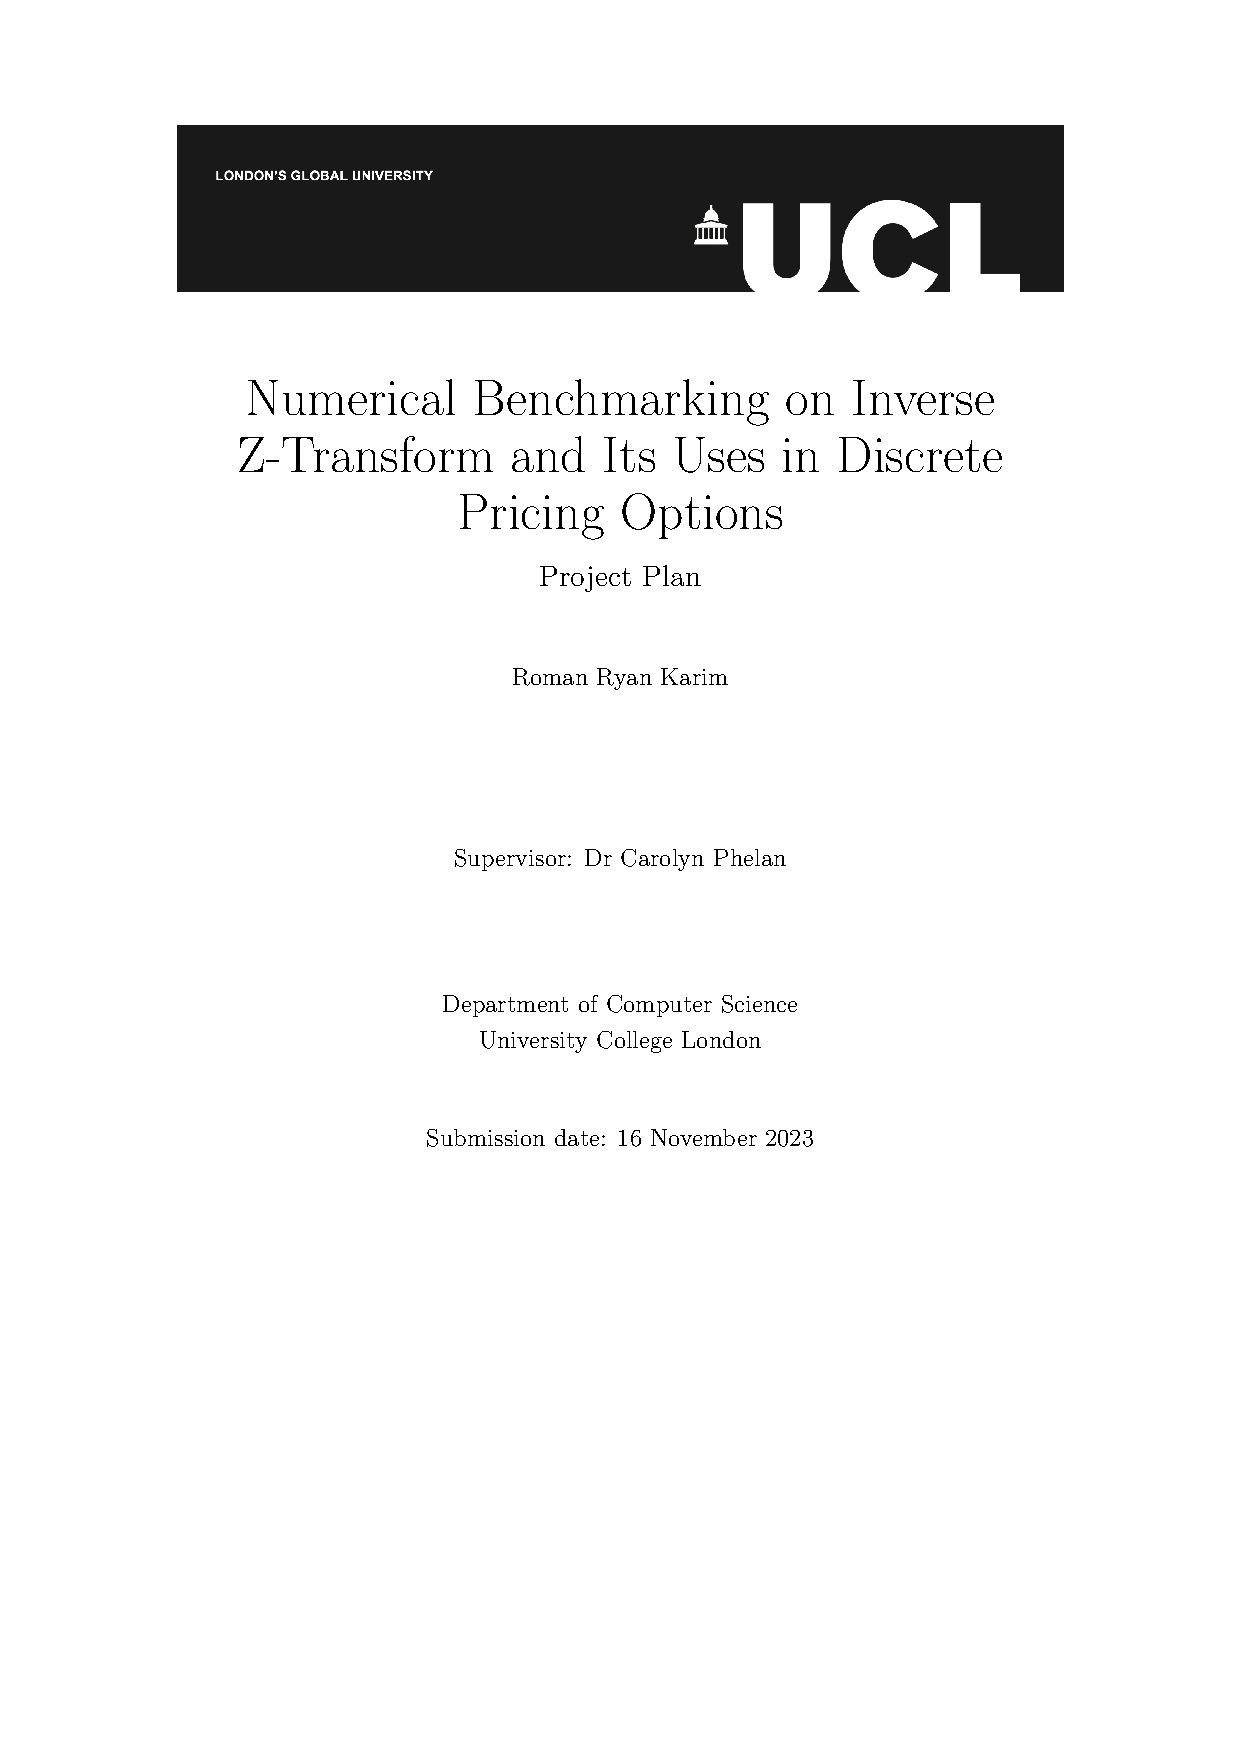
\includepdf[pages=-]{initial_project_plan.pdf}

\chapter{Code Listings}\label{chapter:code_listings}

% ========================================
% Transform Pairs
% ========================================
\section{Transform Pairs}
These transform pairs serve as benchmarks for testing the accuracy and efficiency of numerical inversion methods. Each pair consists of a time-domain function and its corresponding Z-transform, providing a practical basis for analysing and validating the implemented algorithms.

\subsection{Heaviside Step}
\begin{lstlisting}[language=Python, caption= Implementation of the Heaviside Step function and its $\mathcal{Z}$-transform (Section \ref{section:heaviside_step})]
def f(t):
    return 1
    
def ftilde(z):
    return z / (z-1)
\end{lstlisting}

\subsection{Polynomial}
\begin{lstlisting}[language=Python, caption= Implementation of the Polynomial function and its $\mathcal{Z}$-transform (Section \ref{section:polynomial})]
def f(t):
    return t
    
def ftilde(z):
    return z / (z-1)**2
\end{lstlisting}

\subsection{Decaying Exponential}
\begin{lstlisting}[language=Python, caption= Implementation of the Decaying Exp function and its $\mathcal{Z}$-transform (Section \ref{section:decaying_exp})]
def f(a, t):
    return np.exp(-a * t)
    
def ftilde(z, a, t, N):
    delta_t = t / N
    denominator = 1 - np.exp(-a * delta_t) / z
    return 1 / denominator
\end{lstlisting}

\newpage
\subsection{Sinusiodal}
\begin{lstlisting}[language=Python, caption= Implementation of the Sinusoidal function and its $\mathcal{Z}$-transform (Section \ref{section:sinusoidal})]
def f(omega, t):
    return np.sin(omega * t)
    
def ftilde(z, omega, t, N):
    delta_t = t / N
    numerator = z**(-1) * np.sin(omega * delta_t)
    denominator = 1 - 2 * np.cos(omega * delta_t) * z**(-1) + z**(-2)
    return numerator / denominator
\end{lstlisting}

\newpage
\section{Contours}

\subsection{Circular}
\begin{lstlisting}[language=Python, caption= Implementation of a circular contour from $0 \leq \theta < \pi$.]
def circle(r, n):
    z = []
    for k in range(0, n):
        theta = np.pi * k / n
        point = r * np.exp(1j * theta)
        z.append(point)
    return z
\end{lstlisting}

\begin{lstlisting}[language=Python, caption= Implementation of a circular contour from $0 \leq \theta \leq \pi$.]
def circle(r, n):
    z = []
    for k in range(0, n):
        theta = (np.pi + np.pi / n) * k / n
        point = r * np.exp(1j * theta)
        z.append(point)
    return z
\end{lstlisting}

\subsection{Sinh Deformation}
\begin{lstlisting}[language=Python, caption= Implementation of the conformal mapping (Equation \ref{equation:conformal_mapping}) from $-\frac{\pi}{2} \leq \omega < \frac{\pi}{2}$.]
def hyperbolic_sine(sigma, b, y, n):
    z = np.zeros(n, dtype=complex)
    for k in range(n):
        omega = 1j * (-np.pi/2 + k * np.pi / n)
        z[k] = sigma + 1j * b * np.sinh(omega + y)
    return z
\end{lstlisting}

\begin{lstlisting}[language=Python, caption= Implementation of the conformal mapping (Equation \ref{equation:conformal_mapping}) from $-\frac{\pi}{2} \leq \omega \leq \frac{\pi}{2}$.]
def hyperbolic_sine(sigma, b, y, n):
    z = np.zeros(n, dtype=complex)
    for k in range(n):
        omega = 1j * (np.pi) * (k - (n - 1) / 2) / (n - 1)
        z[k] = sigma + 1j * b * np.sinh(omega + y)
    return z
\end{lstlisting}

% ========================================
% Numerical Inverse Z-Transform
% ========================================
\newpage
\section{Numerical Inverse $\mathcal{Z}$-Transform}
We provide the python implementation of the numerical inverse $z$-transform for the methods discussed in Section \ref{section:inverse_z}. The implementations are structured such that we make use of NumPy's vectorised operations in an attempt of achieving the best performance possible.

\subsection{Abate and Whitt 1992}
\begin{lstlisting}[language=Python, caption= Implementation of \citet{AbateWhitt1992a, AbateWhitt1992b}'s NIZT (Equation \ref{eq:aw_inversion}).]
def abate_whitt(ftilde, n, lmbda):
    rho = 10 ** (-lmbda / (2 * n))
    
    k = np.arange(1, n)
    z = 1 / (rho * np.exp(1j * k * np.pi / n))
    summation = 2 * np.sum(((-1) ** k) * np.real(ftilde(z)))
    
    result = (1 / (2 * n * rho ** n)) * (ftilde(1 / rho) + summation + ((-1) ** n) * ftilde(-1 / rho))
    return result
\end{lstlisting}

\subsection{Cavers 1978}
\begin{lstlisting}[language=Python, caption= Implementation of \citet{Cavers1978FFT}'s FFT NIZT (Equation \ref{cavers})]
def cavers(ftilde, n, N, gamma):
    r = 10 ** (gamma / (N))
    k = np.arange(N)
    z = r * np.exp(1j * 2 * np.pi * k / (N))
    F = np.fft.ifft(ftilde(z))
    f = r ** n * F[n]
    return f
\end{lstlisting}

\begin{lstlisting}[language=Python, caption= Implementation of \citet{Cavers1978FFT}'s DFT NIZT (Equation \ref{equation:cavers_sum})]
def cavers_dft(ftilde, n, J, gamma):
    r = 10 ** (gamma / J)
    
    j = np.arange(J)
    z = r * np.exp(1j * 2 * np.pi * j / J)
    
    z_ftilde = ftilde(z)
    z_power = z[:, None] ** n  # Compute z^n for all n and z
    
    f = np.sum(z_power * z_ftilde[:, None], axis=0) / J
    return f
\end{lstlisting}

% ========================================
% Optimisation Techniques
% ========================================
\newpage
\section{Optimisation Techniques}

\subsection{Loss Function}
\begin{lstlisting}[language=Python, caption= null]
def loss(z):
    L1 = np.sum((np.abs(z) - 1) ** 2)
    return L1
\end{lstlisting}

\subsection{Gradient Descent}
\begin{lstlisting}[language=Python, caption= null]
def gradient_descent(N, learning_rate=1e-3, num_iterations=1_000_000):
	# initial values
    b = 0.7
    y = 0.895588
    
    # initialising parameters
    best_loss = float('inf')
    best_b = b
    best_y = y

    for i in range(num_iterations):
        # compute loss
        L1 = loss_function(b, y, N)
        
        if L1 < best_loss:
            best_loss = L1
            best_b = b
            best_y = y
        
        # compute gradients 
        epsilon = 1e-8
        grad_b = (loss_function(b + epsilon, y, N) - L1) / epsilon
        grad_y = (loss_function(b, y + epsilon, N) - L1) / epsilon
        
        # update parameters
        b -= learning_rate * grad_b
        y -= learning_rate * grad_y
    
    return best_b, best_y, best_loss
\end{lstlisting}

\subsection{ADAM Optimiser}
\begin{lstlisting}[language=Python, caption= null]
def adam_optimiser(N, initial_learning_rate=1e-3, num_iterations=1_000_000, beta1=0.9, beta2=0.999, epsilon=1e-5):
	# initial values
    b = 0.14124692711511863
    y = 2.6503746377415633

	# initialising parameters
    best_loss = float('inf')
    best_b = b
    best_y = y
    m_b, v_b = 0, 0
    m_y, v_y = 0, 0
    t = 0

    for i in range(num_iterations):
        t += 1
        
        # compute loss
        L1 = loss_function(b, y, N)
        
        if L1 < best_loss:
            best_loss = L1
            best_b = b
            best_y = y
        
        # compute gradients (estimate)
        grad_b = (loss_function(b + epsilon, y, N) - L1) / epsilon
        grad_y = (loss_function(b, y + epsilon, N) - L1) / epsilon
        
        # update biased first moment
        m_b = beta1 * m_b + (1 - beta1) * grad_b
        m_y = beta1 * m_y + (1 - beta1) * grad_y
        
        # update biased second moment
        v_b = beta2 * v_b + (1 - beta2) * (grad_b ** 2)
        v_y = beta2 * v_y + (1 - beta2) * (grad_y ** 2)
        
        # compute bias-corrected first moment
        m_b_hat = m_b / (1 - beta1 ** t)
        m_y_hat = m_y / (1 - beta1 ** t)
        
        # compute bias-corrected second moment
        v_b_hat = v_b / (1 - beta2 ** t)
        v_y_hat = v_y / (1 - beta2 ** t)
        
        # update parameters
        b -= initial_learning_rate * m_b_hat / (np.sqrt(v_b_hat) + epsilon)
        y -= initial_learning_rate * m_y_hat / (np.sqrt(v_y_hat) + epsilon)
       
    return best_b, best_y, best_loss
\end{lstlisting}

  
\end{appendices}

\end{document}